\documentclass[12.2pt,a4paper]{book}
\usepackage[top=2.2cm, bottom=2.2cm, left=1.8cm, right=1.8cm]{geometry}

\usepackage{lmodern}
\usepackage[table]{xcolor}
\usepackage{xcolor}
\definecolor{vert1}{rgb}{0.0,0.3.9,0.0}
\definecolor{bleu}{rgb}{0,0,0.5}
\definecolor{bleu3}{rgb}{1,0.2,0.2}
\definecolor{grisgris}{gray}{0.4}
\definecolor{grisclair}{HTML}{E7E7E7}
\definecolor{grisfonce}{HTML}{A5A5A5}
\definecolor{rougeUPS}{rgb}{0.6, 0.3, 0.3}

\fboxsep =0pt \parindent =0pt\parskip =12pt



\usepackage[utf8]{inputenc}
\usepackage[T1]{fontenc}
\usepackage[francais]{babel}
\usepackage{verbatim}
\usepackage[urlbordercolor={1 1 1}, linkbordercolor={1 1 1}, linkcolor=vert1, urlcolor=bleu, colorlinks=true]{hyperref}
\usepackage{tikz} %Vectoriel
\usepackage{listings}
\usepackage{fancyhdr}
%\usepackage{amssymb}
\usepackage{eurosym}
\usepackage{float}
\usepackage{graphicx}
\usepackage{pdfpages}
\usepackage{lib/lipsum}
\usepackage{lib/wrapfig}
\lhead{Projet Agile --- \bsc{Scrum}}
\cfoot{\thepage}

\newcommand{\titreRapport}{Refonte du système multi-langue pour une application web}
\newcommand{\mbx}{Memobox~/\-~2G Technologies}
\newcommand{\memobox}{Memobox}
\newcommand{\techno}{2G Technologies}
\newcommand{\adt}{\bsc{AUDITEL}com}

\newcommand{\Adr}{Antoine de \bsc{Roquemaurel}}
\newcommand{\adr}{A. de \bsc{Roquemaurel}}
\newcommand{\Romain}{Romain \bsc{Auriac}}
\newcommand{\Denis}{Denis \bsc{Mallet}}
\newcommand{\romain}{R. \bsc{Auriac}}
\newcommand{\denis}{D. \bsc{Mallet}}
\newcommand{\mlanguage}{\texttt{MemoLanguage}}

\def\vs{\leavevmode\hbox{\tt\char`\ }}

\newcommand{\remarque}[1]{
	\begin{center}
	\medskip
	\colorbox{remarque}{
		\begin{minipage}{0.85\textwidth}\medskip
\includegraphics[height=10px]{images/remarque.png} #1 \medskip\end{minipage}
	}
	\medskip
	\end{center}
}

\newcounter{exemples}

\newenvironment{exemple}[1]{
   \vspace{-2mm}

\refstepcounter{exemples}
   \begin{center}
	\medskip
      \begin{minipage}{0.9\linewidth}
}{%
~
      \end{minipage}
   \end{center}~
   \vspace{-2mm}
}%

\newcommand{\captionExemple}[1]{
	\begin{center}{\bsc{Exemple} \thechapter.\arabic{exemples}~--~}#1\end{center}
}


\DeclareTextFontCommand{\policeGlossaire}{\fontfamily{lmss}\selectfont}
\DeclareTextFontCommand{\policePackage}{\fontfamily{phv}\selectfont}
\DeclareTextFontCommand{\policeTitre}{\fontfamily{ptm}\selectfont}
\newcommand{\policeCode}[1]{\texttt{#1}}

\newcommand{\sectionfont}{%
	\fontencoding{\encodingdefault}%
	\fontfamily{pag}%
	\fontseries{bc}%
	\fontshape{n}%
	\selectfont
}

% numéro du chapitre
\DeclareFixedFont{\chapnumfont}{T1}{phv}{b}{n}{80pt}
% pour le mot « Chapitre »
\DeclareFixedFont{\chapchapfont}{T1}{phv}{b}{n}{16pt}
% pour le titre
\DeclareFixedFont{\chaptitfont}{T1}{phv}{b}{n}{24.88pt}


\makeatletter
\def\thickhrulefill{\leavevmode \leaders \hrule height 1ex \hfill \kern \z@}
%% \chapter
\def\@makechapterhead#1{%
  \reset@font
  \parindent \z@
  \vspace*{10\p@}%
  \hbox{%
    \vbox{%
      \advance\hsize by -2cm
      \hrule height 0.4pt depth 0pt width \hsize
      \par
      \vskip 6pt%
      \hspace{20pt}%
      \parbox{420pt}{%
        \LARGE \bfseries #1
		}%
      \par
      \vskip 6pt%
      \hspace{20pt}%
      \hrule height 0.4pt depth 0pt width \hsize
	  \vspace{-30pt}
      }%
    \vbox{%
      \hsize=1.5cm%
      \begin{tabular}{c}
        \scshape \large \strut \@chapapp{} \\
        \colorbox{black}{\vbox{\hbox{\vbox to 1mm{}}\hbox{
			\color{white} \LARGE \bfseries \hspace{1mm}\thechapter\hspace{1mm}
		}\hbox{\vbox to 2cm{}}}}%
      \end{tabular}%
      }%
    }%
  \vskip 20\p@
}
%% \chapter*
\def\@makeschapterhead#1{%
  \reset@font
  \parindent \z@
  \vspace*{10\p@}%
  \hbox{%
    \vbox{%
      \advance\hsize by -0cm
      \hrule height 0.4pt depth 0pt width \hsize
      \par
      \vskip 6pt%
      \hspace{20pt}%
      \parbox{420pt}{%
        \LARGE \bfseries #1
		}%
      \par
      \vskip 6pt%
      \hspace{20pt}%
      \hrule height 0.4pt depth 0pt width \hsize
      }%
    }%
  \vskip 20\p@

}

\newlength{\sectiontitleindent}
\newlength{\subsectiontitleindent}
\newlength{\subsubsectiontitleindent}
\setlength{\sectiontitleindent}{-1cm}
\setlength{\subsectiontitleindent}{-.5cm}
\setlength{\subsubsectiontitleindent}{-.25cm}

\renewcommand{\section}{%
	\@startsection%
	{section}%
	{1}%
	{\sectiontitleindent}%
	{-3.5ex plus -1ex minus -.2ex}%
	{2.3ex plus.2ex}%
	{\sectionfont\Large}
}
\renewcommand{\subsection}{%
	\@startsection%
	{subsection}%
	{2}%
	{\subsectiontitleindent}%
	{-3.5ex plus -1ex minus -.2ex}%
	{2.3ex plus.2ex}%
	{\sectionfont\large}
}

\renewcommand{\subsubsection}{%
	\@startsection%
	{subsubsection}%
	{3}%
	{\subsubsectiontitleindent}%
	{-3.5ex plus -1ex minus -.2ex}%
	{2.3ex plus.2ex}%
	{\sectionfont\normalsize}
}

\makeatother






\definecolor{gris1}{gray}{0.40}
\definecolor{gris2}{gray}{0.55}
\definecolor{gris3}{gray}{0.65}
\definecolor{gris4}{gray}{0.50}
\definecolor{vert}{rgb}{0,0.4,0}
\definecolor{violet}{rgb}{0.65, 0.2, 0.65}
\definecolor{bleu1}{rgb}{0,0,0.8}
\definecolor{bleu2}{rgb}{0,0.2,0.6}
\definecolor{bleu3}{rgb}{0,0.2,0.2}
\definecolor{rouge}{HTML}{F93928}


\lstdefinelanguage{algo}{%
   morekeywords={%
    %%% couleur 1
		importer, programme, glossaire, fonction, procedure, constante, type, 
	%%% IMPORT & Co.
		si, sinon, alors, fin, tantque, debut, faire, lorsque, fin lorsque, 
		declenche, declencher, enregistrement, tableau, retourne, retourner, =, pour, a,
		/=, <, >, traite,exception, 
	%%% types 
		Entier, Reel, Booleen, Caractere, Réél, Booléen, Caractère,
	%%% types 
		entree, maj, sortie,entrée,
	%%% types 
		et, ou, non,
	},
  sensitive=true,
  morecomment=[l]{--},
  morestring=[b]',
}

\lstset{language=algo,
    %%% BOUCLE, TEST & Co.
      emph={importer, programme, glossaire, fonction, procedure, constante, type},
      emphstyle=\color{bleu2},
    %%% IMPORT & Co.  
	emph={[2]
		si, sinon, alors, fin , tantque, debut, faire, lorsque, fin lorsque, 
		declencher, retourner, et, ou, non,enregistrement, retourner, retourne, 
		tableau, /=, <, =, >, traite,exception, pour, a
	},
      emphstyle=[2]\color{bleu1},
    %%% FONCTIONS NUMERIQUES
      emph={[3]Entier, Reel, Booleen, Caractere, Booléen, Réél, Caractère},
      emphstyle=[3]\color{gris1},
    %%% FONCTIONS NUMERIQUES
      emph={[4]entree, maj, sortie, entrée},	
      emphstyle=[4]\color{gris1},
}
\lstdefinelanguage{wl}{%
   morekeywords={%
    %%% couleur 1
		importer, programme, glossaire, fonction, procedure, constante, type, 
	%%% IMPORT & Co.
		si, sinon, alors, fin, TANTQUE, tantque, FIN, PROCEDURE, debut, faire, lorsque, 
		fin lorsque, declenche, declencher, enregistrement, tableau, retourne, retourner, =, 
		/=, <, >, traite,exception, 
	%%% types 
		Entier, Reel, Booleen, Caractere, Réél, Booléen, Caractère,
	%%% types 
		entree, maj, sortie,entrée,
	%%% types 
		et, ou, non,
	},
  sensitive=true,
  morecomment=[l]{//},
  morestring=[b]',
}

\lstset{language=wl,
    %%% BOUCLE, TEST & Co.
      emph={importer, programme, glossaire, fonction, procedure, constante, type},
      emphstyle=\color{bleu2},
    %%% IMPORT & Co.  
	emph={[2]
		si, sinon, alors, fin , tantque, debut, faire, lorsque, fin lorsque, 
		declencher, retourner, et, ou, non,enregistrement, retourner, retourne, 
		tableau, /=, <, =, >, traite,exception
	},
      emphstyle=[2]\color{bleu1},
    %%% FONCTIONS NUMERIQUES
      emph={[3]Entier, Reel, Booleen, Caractere, Booléen, Réél, Caractère},
      emphstyle=[3]\color{gris1},
    %%% FONCTIONS NUMERIQUES
      emph={[4]entree, maj, sortie, entrée},	
      emphstyle=[4]\color{gris1},
}
\lstdefinelanguage{css}{%
   morekeywords={%
    %%% couleur 1
		background, image, repeat, position, index, color, border, font, 
		size, url, family, style, variant, weight, letter, spacing, line, 
		height, text, decoration, align, indent, transform, shadow, 
		background, image, repeat, position, index, color, border, font, 
		size, url, family, style, variant, weight, letter, spacing, line, 
		height, text, decoration, align, indent, transform, shadow, 
		vertical, align, white, space, word, spacing,attachment, width, 
		max, min, margin, padding, clip, direction, display, overflow,
		visibility, clear, float, top, right, bottom, left, list, type, 
		collapse, side, empty, cells, table, layout, cursor, marks, page, break,
		before, after, inside, orphans, windows, azimuth, after, before, cue, 
		elevation, pause, play, during, pitch, range, richness, spek, header, 
		numeral, punctuation, rate, stress, voice, volume,
	%%% types 
		left, right, bottom, top, none, center, solid, black, blue, red, green,
	},
  sensitive=true,
  sensitive=true,
  morecomment=[s]{/*}{*/},
  morestring=[b]',
}
\lstset{language=css,
    %%% BOUCLE, TEST & Co.
      emph={
		background, image, repeat, position, index, color, border, font, 
		size, url, family, style, variant, weight, letter, spacing, line, 
		height, text, decoration, align, indent, transform, shadow, 
		background, image, repeat, position, index, color, border, font, 
		size, url, family, style, variant, weight, letter, spacing, line, 
		height, text, decoration, align, indent, transform, shadow, 
		vertical, align, white, space, word, spacing,attachment, width, 
		max, min, margin, padding, clip, direction, display, overflow,
		visibility, clear, float, top, right, bottom, left, list, type, 
		collapse, side, empty, cells, table, layout, cursor, marks, page, break,
		before, after, inside, orphans, windows, azimuth, after, before, cue, 
		elevation, pause, play, during, pitch, range, richness, spek, header, 
		numeral, punctuation, rate, stress, voice, volume,
	  },
      emphstyle=\color{bleu2},
    %%% FONCTIONS NUMERIQUES
      emph={[3]
		left, right, bottom, top,none, solid, black, blue, green,
		  },
      emphstyle=[3]\color{bleu3},
    %%% FONCTIONS NUMERIQUES
}

\lstset{language=SQL,
    %%% BOUCLE, TEST & Co.
      emph={INSERT, UPDATE, DELETE, WHERE, SET, GROUP, BY, ORDER, REFERENCES},
      emphstyle=\color{bleu2},
    %%% IMPORT & Co.  
	emph={[2]
		if, end, begin, then, for, each, else, after, of, on, to
	},
      emphstyle=[2]\color{bleu1},
    %%% FONCTIONS NUMERIQUES
      emph={[3]Entier, Reel, Booleen, Caractere, Booléen, Réél, Caractère},
      emphstyle=[3]\color{gris1},
    %%% FONCTIONS NUMERIQUES
      emph={[4]entree, maj, sortie, entrée},	
      emphstyle=[4]\color{gris1},
}
\lstdefinelanguage{ARM}{%
   morekeywords={%
   ADD, SUB, MOV, MUL, RSB,CMP, BLS, BLE, B,BHI,LDR,
   BGE, RSBLT, BGT, BEQ, BNE,BLT,BHS,STR,STRB
	},
  sensitive=true,
  morecomment=[l]{@},
  morestring=[b]',
}

\lstset{ % general style for listings 
   numbers=left 
   , literate={é}{{\'e}}1 {è}{{\`e}}1 {à}{{\`a}}1 {ê}{{\^e}}1 {É}{{\'E}}1 {ô}{{\^o}}1 {€}{{\euro}}1{°}{{$^{\circ}$}}1 {ç}{ {c}}1 {ù}{u}1
	, extendedchars=\true
   , tabsize=2 
   , frame=l
   , framerule=1.1pt
   , linewidth=520px
   , breaklines=true 
   , basicstyle=\footnotesize\ttfamily 
   , numberstyle=\tiny\ttfamily 
   , framexleftmargin=0mm 
   , xleftmargin=0mm 
   , captionpos=b 
	, keywordstyle=\color{bleu2}
	, commentstyle=\color{vert}
	, stringstyle=\color{rouge}
	, showstringspaces=false
	, extendedchars=true
	, mathescape=true
} 
%	\lstlistoflistings
%	\addcontentsline{toc}{part}{List of code examples}



\makeatletter
\addto\captionsfrench{%
  \renewcommand\listfigurename{Liste des figures}%
}

\newcommand\tableofcontentsA{%
	\chapter*{Table des annexes
	\@mkboth{%
	\MakeUppercase\contentsname}{\MakeUppercase\contentsname}}%
	\@starttoc{toca}%
}
\renewcommand*{\lstlistlistingname}{Liste des codes sources}
\addto\captionsenglish{\renewcommand{\figurename}{Fig.}}

% replace : with . in caption
\renewcommand{\@makecaption}[2]{%
\vspace{\abovecaptionskip}%
\sbox{\@tempboxa}{#1. #2}
\ifdim\wd\@tempboxa > \hsize
        #1. #2\par
\else
        \global\@minipagefalse
        \hbox to \hsize {\hfil #1. #2\hfil}%
\fi
\vspace{\belowcaptionskip}}%

% make lof a subsubsection
\renewcommand\listoffigures{%
    \chapter{\listfigurename}%
      \@mkboth{\MakeUppercase\listfigurename}%
              {\MakeUppercase\listfigurename}%
       \@starttoc{lof}%
    }
    \renewcommand\listoftables{%
    \chapter{\listtablename}%
    \@mkboth{\MakeUppercase{\listtablename}}%
            {\MakeUppercase{\listtablename}}%
    \@starttoc{lot}
    }

    \renewcommand\lstlistoflistings{%
    \begingroup
    \chapter{\lstlistlistingname}%
    \parskip\z@\parindent\z@\parfillskip \z@ \@plus 1fil%
    \@starttoc{lol}%
    \endgroup
    }
\makeatother

\includeonly{
	contenu/0-avantPropos/pageDeTitre,
	contenu/0-avantPropos/remerciements,
	contenu/0-avantPropos/intro,
	contenu/1-entreprise,
	contenu/3-mission,
	contenu/4-bilan,
%
%   contenu/annexes/preambule,
 %  contenu/annexes/pageDeTitre,
%   contenu/annexes/resultats,
%  contenu/annexes/codeSource,
%  contenu/annexes/glossaire,
%  contenu/annexes/listes,
}
\begin{document}
\thispagestyle{empty}
	\setcounter{tocdepth}{1}
	\setcounter{secnumdepth}{3}
	
		
\includepdf{styles/couverture_annexes.pdf} %Couverture du rapport de stage
	\newpage
	\begin{flushright}
		~
		\vfill
		\vspace{200px}
		Version du \today{}
	\end{flushright}
	\thispagestyle{empty}
    \newpage
\sffamily
	\vspace{10px}
\thispagestyle{empty}
	%
	%
	% Pour éviter de créer un nouveau paragraph, on commente les lignes vide
		\vspace{30px}
		%
		\mbox{}\hfill{
			\begin{flushright}
				\fontsize{15}{15} \selectfont Antoine de \bsc{Roquemaurel}\\\vspace{10px}
				\fontsize{10}{10} \selectfont Stage effectué chez Memobox -- 2G technologies\\
				Du 10 Avril 2012 au 22 Juin 2012
			\end{flushright}
			\begin{flushleft}
				Pour M. Denis \bsc{Mallet}\\
				Pour M. Patrick \bsc{Magnaud}\\
			\end{flushleft}
		}\par
		%
		\vfill\mbox{}\vfill
		%
		%
		\vfill
		\vfill
		\vfill
		\vfill
		\vfill
		\hspace{65px}
		\fbox{
		\begin{minipage}{0.7\textwidth}
			\begin{center}
				\vspace{20px}	
				\fontsize{35}{25}\selectfont Rapport de stage
				
				\fontsize{22}{22}\selectfont \titreRapport
				\vspace{20px}	
			\end{center}
		\end{minipage}
		}
		%
%		\hrule height 4pt
		%
		\begin{center}
			\fontsize{20}{20}\selectfont\vspace{20px} --- Annexes ---
		\end{center}
		% Les vfill servent à insérer du blanc en dessous du titre pour éviter que le titre aille tout en bas
		% Plus il y a de vFill plus le titre sera haut dans la page
	% Le cadre sur la gauche, une boite rouge avec les logos IUT et UPS
		\vfill
		\vfill
		\vfill
		\vfill
		\vfill
		\vfill
		\vfill
	\begin{flushleft}
		\fontsize{11.5}{11.5}\selectfont
		Memobox -- 2G Technologies\\
		12 Bv de l'Europe\\
		31850 -- \bsc{Montrabé}\\
		
\includegraphics[width=4.5cm]{images/logoMemobox.png}\\%
	\end{flushleft}
		\vfill
		\vfill
		\vfill
		\vfill
		\mbox{}
		
\newpage
~
\thispagestyle{empty}

	 \tableofcontentsA
	 \newpage
	\thispagestyle{empty}
	\renewcommand{\chaptermark}[1]{\markboth{\bsc{Annexe~\thechapter{} :} #1}{}}
	\chapter*{Remerciements}
\addcontentsline{toc}{chapter}{Remerciements}%%
\`A l'issue de ce stage, je me rend compte que je ne pourrais pas être
là ou j'en suis sans certaines personnes, à qui je désire témoigner ma reconnaissance.

Je tiens tout d'abord à remercier l'entreprise \mbx{} de m'avoir accueilli chaleureusement pour mon stage.
Merci tout particulièrement à \Denis{}, mon maître de stage, qui a su me guider lors de ces deux mois et me permettre de continuer l'aventure au mois de Juillet.

Ma gratitude va à \Romain{} pour m'avoir aidé dans mon projet et m'avoir conseillé tout au long du stage, mais également de m'avoir rapidement intégré dans l'équipe de développement.

Je suis reconnaissant envers Monsieur Patrick \bsc{Magnaud}, professeur tuteur, de m'avoir suivi et d'être venu au cours de ce stage.

Merci également à Olga \bsc{Bensadoun} pour m'avoir proposé ce stage.

Mes remerciements vont également à tous les membres de l'Institut Universitaire de Technologies 'A' de Toulouse, professeurs et membres du service techniques sans qui je ne serais pas là aujourd'hui.

Je remercie Mathieu \bsc{Soum}, qui effectuais son stage dans les locaux de l'entreprise, pour ses conseils, et nos moments de détentes toujours sympathiques autour d'un petit café.

Enfin, je remercie Diane \bsc{Auzet} pour avoir eu la gentillesse de relire ce rapport.




	\chapter*{Avant-propos}
\nouveauChapitre
\addcontentsline{toc}{chapter}{Avant-propos}
\section*{Présentation du projet}
\addcontentsline{toc}{section}{Présentation du projet}
	LibUML est une 
	\glo{bibliothèque}{Bibliothèque}{Composant programmé dans un langage donné fournissant des méthodes permettant d'effectuer des tâches voulus} 
	d'objets graphiques représentant les différents éléments de modélisation de la norme 
	\glo{UML}{UML}{(Unified Modeling Language) Langage de modélisation graphique à base de pictogramme.  Il est apparu dans le monde du génie logiciel dans le cadre de la conception orientée objet. Ce langage est composé de différents diagrammes, allant du développement à la simple ana\-lyse des besoins.} 
	2\footnote{Unified Modelling Language}.
	Celle-ci a été développé dans le cadre des projets tuteurés à l'IUT\footnote{Institut Universitaire de Technologies} 'A' de Toulouse. 
	Nous l'avons développée en \glo{Java}{Java}{Langage de programmation orienté objet moderne, il compile le programme pour ensuite l'exécuter sur une machine Java, ainsi le programme une fois compilé peut être exécuté sur différentes plateformes (Windows, Linux, Mac OS X, \ldots).} 
	et conçue comme une bibliothèque pouvant être utilisée dans des programmes Java comme composant. 
	Vous pouvez vous en servir pour développer un outil complet de modélisation UML par exemple.
	\paragraph{}	
	Cette bibliothèque permet de faire différentes choses dans le cadre de la conception UML, une fois que vous aurez compris le fonctionnement de libUML vous pourrez:
	\begin{itemize}
		\item Créer des éléments de modélisation 
			\begin{itemize}
				\item Acteur actif ou passif
				\item Traitement
				\item Cas d'utilisation
				\item Classe
			\end{itemize}
		\item Relier ses composants via différents types de flèches
			\begin{itemize}
				\item Agrégation
				\item Composition
				\item Association binavigable ou mononavigable
				\item Messages synchrones ou asynchrones
				\item Généralisation
			\end{itemize}
		\item Supprimer des éléments et flèches
		\item Modifier le contenu des éléments et flèches
		\item Redimensionner les éléments de modélisation
	\end{itemize}
	\paragraph{}
Ce document a pour but de vous présenter le fonctionnement de la bibliothèque UML et de son démonstrateur. 

\section*{Présentation du groupe}
\addcontentsline{toc}{section}{Présentation du groupe}
	Notre groupe projet est composé de quatre étudiants de deuxième année de DUT Informatique à l'IUT 'A' de Toulouse, voici la composition de l'équipe: 
	\begin{itemize}
		\item Antoine de \bsc{Roquemaurel} 
		\item Mathieu \bsc{Soum} 
		\item Geoffroy \bsc{Subias}
		\item Marie-Ly \bsc{Tang} 
	\end{itemize}
	\section*{Téléchargements}
\addcontentsline{toc}{section}{Téléchargements}
	Nous vous avons envoyé deux archives zip par email, une contenant le projet Netbeans de la bibliothèque et du démonstrateur et une contenant la bibliothèque.
	\subsubsection*{Bibliothèque et démonstrateur}
	La première archive est donc un projet netbeans, cette archive contient notre bibliothèque et ses tests associés, le démonstrauteur mais
	également la bibliothèque \texttt{JGraphx} qui est indispensable au bon fonctionnement de notre bibliothèque. Nous ne garantissons le bon fonctionnement 
	de la bibliothèque qu'avec la version de \texttt{JGraphx} 1.8, celle-ci n'ayant pas été testée avec des versions différentes.

	Le projet netbeans de notre bibliothèque est également disponible en ligne, si vous souhaitez la télécharger de nouveau, elle est donc disponible à l'adresse suivante: \\
	$\rhd$ \url{http://telechargements.joohoo.fr/libUML/libUML-netbeans.zip}\\
	$\rhd$ \url{http://telechargements.joohoo.fr/libUML/JGraphX-1.8.jar}\\
	
	\subsubsection*{Documentation}
	Toute la documentation du projet est sous format \bsc{HTML}\footnote{HyperText Markup Language}, celle-ci ayant été générée grâce à Javadoc.

	Si dans ce manuel nous parlons d'une méthode et que vous n'en comprenez pas l'intéret, vous pouvez aller la chercher dans la documentation, pour chaque classe,
	le fonctionnement global de la classe est expliquée, l'utilité de chaque attribut, de chaque méthode, et ce que vous devez mettre dans les différents paramètres 
	des méthodes.  
	\paragraph{}
	Nous vous avons remis un .zip par email contenant quatre dossiers de documentation:
	\begin{itemize}
		\item La documentation privée de la \textit{bibliothèque} (Toutes les méthodes et tous les attributs)
		\item La documentation publique de la \textit{bibliothèque} (Seuls les méthodes et attributs publics ou protégés)
		\item La documentation privée du \textit{démonstrateur} (toutes les méthodes du démonstrateur) 
		\item La documentation des \textit{tests unitaires} (Toutes les méthodes de tests)
	\end{itemize}
	\paragraph{}
	Celle ci est également disponible en ligne aux adresses suivantes: \\
	$\rhd$ \url{http://documentation.joohoo.fr/libUML/bibliothequePrivee/index.html}\\
	$\rhd$ \url{http://documentation.joohoo.fr/libUML/bibliothequePublique/index.html}\\
	$\rhd$ \url{http://documentation.joohoo.fr/libUML/demonstrateurPrivee/index.html}\\\label{docDemonstrateur}
	$\rhd$ \url{http://documentation.joohoo.fr/libUML/testsUnitaires/index.html}\\
	\paragraph{}
	Vous pouvez également accéder à la documentation de \texttt{JGraphX}, cela peut vous être utile dans certains cas.\\
	$\rhd$ \url{http://documentation.joohoo.fr/JGraphX/index.html}\\ 


	\newpage
\section*{Fonctionnement du document}
\addcontentsline{toc}{section}{Fonctionnement du document}
Ce document est un document expliquant notre approche pour développer une bibliothèque d'objets graphiques UML.\\

Dans ce dossier, vous pourrez repérer diverses notations, cette partie a pour but de vous expliquer les notations afin
que vous puissiez lire en toute sérénité.
\subsubsection*{Le glossaire}
Un mot dans le glossaire a une police particulière, vous pourrez savoir qu'un mot est dans le glossaire lorsque vous repérerez un mot avec la police suivante: 
\policeGlossaire{leMotDansLeGlossiare}. Si vous voyez cette police, vous pouvez donc vous référez à l'annexe \ref{glossaire} page \pageref{glossaire}.
\subsubsection*{Les noms de méthode, d'attribut ou de classe}
Les mots se référant à un nom présent dans du code ont une police particulière, une police type ``machine à écrire'', si vous voyez la police suivante, c'est que c'est un nom 
de méthode, d'attribut ou de classe: \texttt{uneFonction}.
\subsubsection*{Les noms de paquetage}
Les noms de paquetage utiliseront une police particulière, afin que l'on puisse les différencier d'une classe ou d'une méthode, vous les trouverez 
comme suit : \policePackage{unPaquetage}.
\subsubsection*{Les notes de bas de page}
Nous utilisons régulièrement des notes de bas de pages, pour donner un acronyme, pour expliquer plus en détail une notion, ces notes de bas de pages sont un numéro
en exposant, vous trouverez la note correspondante en bas de la page courante, comme ceci\footnote{Ceci est une note de bas de page}.
\subsubsection*{Les liens hypertextes}
Dans le document, nous pouvons faire référence à un lien d'un site web, tous les liens seront donc symbolisés par une petite puce, et une police particulière comme ceci:\\
	$\rhd$ \url{http://monLien.fr/index.html}\\
	Une liste de tous les liens présents dans le document est accessible en annexe \ref{listeLiens} page \pageref{listeLiens}.


	\chapter{Le groupe \mbx{}}
% TODO relecture
	\section{L'historique}
	\begin{description}
		\item[1994] : Création de \memobox{}\\
			\`A l'origine de \memobox{}, deux spécialistes, l'un des services de télécommunications: Christophe \bsc{Fornès} et l'autre du service réseaux: Denis \bsc{Mallet}.\\
			Ensemble, ils décident en 1994 de développer et commercialiser leur propre ligne d'interfaces de communication pour PBX: EdelBox.\\
			Ces interfaces sont commercialisées auprès des éditeurs de logiciels de taxation et d'analyse de trafic téléphonique.

			\memobox{} est né et ne compte aucun salarié.
		
		\item[1995] : Développement commercial\\
			Poussé par ses premiers clients, \memobox{} étend sa gamme en créant un système de taxation téléphonique autonome pour les TPE\footnote{Très Petites Entreprises} et PME\footnote{Petites et Moyennes Entreprises} : Taxabox, décliné également en version hôtelière (Hotelbox).
			Pour se faire, l'entreprise embauche son premier salarié pour étendre ses capacités de développement.
			
		\item[1997] : Le pari du service avec \adt{}\\
			\`A cette date, \memobox{} compte 3 salariés. Après le succès rencontré auprès des éditeurs
			de logiciels et intégrateurs en télécoms, \memobox{} pressant le besoin des entreprises en matière de gestion des coûts télécoms et pour s'adapter
			à son marché, décide de lancer \adt{} le premier service de GFT\footnote{Gestion Financière des Télécoms} en mode hébergé. Une augmentation de capital accompagne ce nouvel axe de développement.
			
		\item[2003] : \memobox{} renforce sa position\\
			Le déploiement des 800 premiers sites nationaux du Ministère de l'Intérieur est bouclé en 4 mois
			et le service satisfait pleinement le client. Pour réaliser cette prouesse, \memobox{} a consolidé ses équipes de développement et d'exploitation.  L'effectif est porté à 13 personnes.
			
		\item[2004] : Les deux fondateurs de \memobox{} rachètent la totalité de l'entreprise.\\
			La bonne santé de \memobox{} en 2004 permet à Christophe \bsc{Fornès} et Denis \bsc{Mallet} de racheter à Global Concept la totalité des parts
			que ce dernier détenait dans l'entreprise. La société est désormais filiale à 100\% du groupe TELECOMS FM\footnote{\textit{Facilities Management}} dont Christophe
			\bsc{Fornès} et Denis \bsc{Mallet} sont les deux seuls actionnaires. \adt{} compte maintenant plus de 2500 sites raccordés et représente désormais 91\% du chiffre d'affaire
			de la société.

		\item[2007] : \memobox{} renforce sa stratégie\\
		Forte de sa politique de développement, \memobox{} décide de renforcer sa stratégie :
		\begin{itemize}
			\item En octobre 2007, elle rachète \techno{} à sa maison mère, \bsc{QUESCOM}.
			\item En décembre 2007, elle lève un million d'euros auprès d'\bsc{ALTO} Invest.
		\end{itemize}
	\end{description}
	\section{La mission de \mbx{}}
	\mbx{} est un éditeur de solutions de \bsc{GFT} et de\textit{ Call Accounting.}
	Forts de leur expérience sur le marché, les deux fondateurs de l'entreprise propose à ses clients une gamme complète d’applications, et de services performants et adaptés aux évolutions permanentes du marché des télécoms.
\newpage	
	La société possède un large panel de clientèle : %%%
	\begin{itemize}
		\item Intégrateurs télécoms,
		\item Prestataires de services,
		\item TPE/PME,
		\item Grandes entreprises,
		\item Administrations et organismes publics.
	\end{itemize}

	La volonté de \mbx{} est également d’être à l’écoute des entreprises pour les conseiller et leur proposer les solutions les mieux adaptées à
	leur besoins. Dans cette optique, ils proposent de nombreuses alternatives à leurs clients en terme de gammes\footnote{logiciels pour PME,
	grands comptes, hôtels, hôpitaux} mais aussi en terme de modes d’installation\footnote{appliances, logiciels ou services externalisés}.

	Ils fournissent aussi des prestations d’administration et d’audit de leurs outils pour permettre aux clients de se concentrer sur le
	c\oe{}ur de leur métier et bénéficier de conseils d’experts avisés.
	
	\section{Les produits de l'entreprise}
		\subsection{Les produits de \techno{}}
		\techno{} a développé les gammes de logiciels suivants:
		\begin{description}	
			\item[GeoTaxe ES] Progiciel destiné aux grandes sociétés, comportant une machine hébergée par les clients collectant leurs données pour les mettre à leurs dispositions via leurs infrastructures internet.
			\item[Geotel] Gestion des appels téléphoniques dans les chambres d'hôtel
			\item[Geopital] Gestion des appels téléphoniques en milieu médicalisé
			\item[Geovox] Serveurs vocaux d'entreprise
		\end{description}
		\subsection{Les produits de \memobox{}}
		\memobox{} a développé les gammes de logiciel suivants:
		\begin{description}	
			\item[\adt{}] Application sous forme de service destinés aux grands comptes
			\item[AUDITELbox] Appliance à installer chez le client de petite taille. Il permet la réalisation d'un audit des télécoms en temps réel.
		\end{description}

	\section{Organisation dans la société}
	\subsection{Mon rôle dans la société}
		J'ai intégré l'équipe de développement de \adt{}, en effet, mon sujet de stage était de refondre le système multi-langues de \adt{}. L'équipe de développement du projet était composée de \Romain{} et de \Denis{}, je me suis rapidement intégré
à l'équipe et ai apporté ma contribution au projet.

\newpage
	\subsection{Le personnel du groupe de Toulouse}
	\begin{description}
		\item[\Denis{}] Vice-président et Directeur Technique
		\item[Jean-Marie \bsc{Lagarde}] Responsable R\&D
		\item[Philippe \bsc{Dureux}] Ingénieur télécoms
		\item[\Romain{}] Ingénieur développement Web
		\item[Mathieu \bsc{Soum}] Stagiaire dans le développement logiciel
		\item[\Adr{}] Stagiaire dans le développement web
	\end{description}
	L'organigramme est disponible figure \ref{organigramme}.
	\begin{figure}[H]
		\centering
		% Graphic for TeX using PGF
% Title: /home/mathieu/businessPlanKlimasoft/includes/Organigramme.dia
% Creator: Dia v0.97.1
% CreationDate: Sat Mar 24 16:53:15 2012
% For: mathieu
% \usepackage{tikz}
% The following commands are not supported in PSTricks at present
% We define them conditionally, so when they are implemented,
% this pgf file will use them.
\ifx\du\undefined
  \newlength{\du}
\fi
\setlength{\du}{15\unitlength}
\begin{tikzpicture}
\pgftransformxscale{1.000000}
\pgftransformyscale{-1.000000}
\definecolor{dialinecolor}{rgb}{0.000000, 0.000000, 0.000000}
\pgfsetstrokecolor{dialinecolor}
\definecolor{dialinecolor}{rgb}{1.000000, 1.000000, 1.000000}
\pgfsetfillcolor{dialinecolor}
\definecolor{dialinecolor}{rgb}{1.000000, 1.000000, 1.000000}
\pgfsetfillcolor{dialinecolor}
\pgfpathellipse{\pgfpoint{37.959375\du}{9.878125\du}}{\pgfpoint{3.450000\du}{0\du}}{\pgfpoint{0\du}{4.475000\du}}
\pgfusepath{fill}
\pgfsetlinewidth{0.050000\du}
\pgfsetdash{}{0pt}
\pgfsetdash{}{0pt}
\definecolor{dialinecolor}{rgb}{0.000000, 0.000000, 0.000000}
\pgfsetstrokecolor{dialinecolor}
\pgfpathellipse{\pgfpoint{37.959375\du}{9.878125\du}}{\pgfpoint{3.450000\du}{0\du}}{\pgfpoint{0\du}{4.475000\du}}
\pgfusepath{stroke}
\pgfsetlinewidth{0.050000\du}
\pgfsetdash{}{0pt}
\pgfsetdash{}{0pt}
\pgfsetbuttcap
\pgfsetmiterjoin
\pgfsetlinewidth{0.000500\du}
\pgfsetbuttcap
\pgfsetmiterjoin
\pgfsetdash{}{0pt}
\definecolor{dialinecolor}{rgb}{1.000000, 0.823529, 0.333333}
\pgfsetfillcolor{dialinecolor}
\pgfpathmoveto{\pgfpoint{37.367856\du}{3.584915\du}}
\pgfpathlineto{\pgfpoint{37.380790\du}{3.597287\du}}
\pgfpathlineto{\pgfpoint{37.325680\du}{3.677984\du}}
\pgfpathlineto{\pgfpoint{37.325680\du}{3.708914\du}}
\pgfpathlineto{\pgfpoint{37.398785\du}{3.752496\du}}
\pgfpathlineto{\pgfpoint{37.423529\du}{3.746310\du}}
\pgfpathlineto{\pgfpoint{37.472172\du}{3.646774\du}}
\pgfpathlineto{\pgfpoint{37.490448\du}{3.659146\du}}
\pgfpathlineto{\pgfpoint{37.661403\du}{3.317799\du}}
\pgfpathlineto{\pgfpoint{37.661403\du}{3.814636\du}}
\pgfpathlineto{\pgfpoint{37.697956\du}{3.814636\du}}
\pgfpathlineto{\pgfpoint{37.490448\du}{4.522635\du}}
\pgfpathlineto{\pgfpoint{37.521378\du}{4.547660\du}}
\pgfpathlineto{\pgfpoint{37.417062\du}{4.566217\du}}
\pgfpathlineto{\pgfpoint{37.350142\du}{4.615985\du}}
\pgfpathlineto{\pgfpoint{37.350142\du}{4.671658\du}}
\pgfpathlineto{\pgfpoint{37.667589\du}{4.671658\du}}
\pgfpathlineto{\pgfpoint{37.673494\du}{4.622171\du}}
\pgfpathlineto{\pgfpoint{37.667589\du}{4.584775\du}}
\pgfpathlineto{\pgfpoint{37.704142\du}{4.578589\du}}
\pgfpathlineto{\pgfpoint{37.881001\du}{4.025798\du}}
\pgfpathlineto{\pgfpoint{38.058423\du}{4.578589\du}}
\pgfpathlineto{\pgfpoint{38.094975\du}{4.584775\du}}
\pgfpathlineto{\pgfpoint{38.088508\du}{4.628357\du}}
\pgfpathlineto{\pgfpoint{38.100880\du}{4.671658\du}}
\pgfpathlineto{\pgfpoint{38.412422\du}{4.671658\du}}
\pgfpathlineto{\pgfpoint{38.412422\du}{4.615985\du}}
\pgfpathlineto{\pgfpoint{38.344940\du}{4.566217\du}}
\pgfpathlineto{\pgfpoint{38.241186\du}{4.547660\du}}
\pgfpathlineto{\pgfpoint{38.265930\du}{4.522635\du}}
\pgfpathlineto{\pgfpoint{38.064046\du}{3.814636\du}}
\pgfpathlineto{\pgfpoint{38.100880\du}{3.814636\du}}
\pgfpathlineto{\pgfpoint{38.100880\du}{3.317799\du}}
\pgfpathlineto{\pgfpoint{38.265930\du}{3.665613\du}}
\pgfpathlineto{\pgfpoint{38.284487\du}{3.646774\du}}
\pgfpathlineto{\pgfpoint{38.332850\du}{3.746310\du}}
\pgfpathlineto{\pgfpoint{38.363779\du}{3.752496\du}}
\pgfpathlineto{\pgfpoint{38.436603\du}{3.708914\du}}
\pgfpathlineto{\pgfpoint{38.436603\du}{3.677984\du}}
\pgfpathlineto{\pgfpoint{38.381774\du}{3.597287\du}}
\pgfpathlineto{\pgfpoint{38.394146\du}{3.584915\du}}
\pgfpathlineto{\pgfpoint{38.131528\du}{3.056868\du}}
\pgfpathlineto{\pgfpoint{37.979131\du}{3.056868\du}}
\pgfpathlineto{\pgfpoint{37.930207\du}{3.007100\du}}
\pgfpathlineto{\pgfpoint{37.814081\du}{3.007100\du}}
\pgfpathlineto{\pgfpoint{37.771343\du}{3.056868\du}}
\pgfpathlineto{\pgfpoint{37.631036\du}{3.056868\du}}
\pgfpathlineto{\pgfpoint{37.367856\du}{3.584915\du}}
\pgfusepath{fill}
\pgfsetbuttcap
\pgfsetmiterjoin
\pgfsetdash{}{0pt}
\definecolor{dialinecolor}{rgb}{1.000000, 0.823529, 0.333333}
\pgfsetfillcolor{dialinecolor}
\pgfpathmoveto{\pgfpoint{37.374604\du}{3.590820\du}}
\pgfpathlineto{\pgfpoint{37.386695\du}{3.603473\du}}
\pgfpathlineto{\pgfpoint{37.331866\du}{3.684170\du}}
\pgfpathlineto{\pgfpoint{37.331866\du}{3.715381\du}}
\pgfpathlineto{\pgfpoint{37.404690\du}{3.758682\du}}
\pgfpathlineto{\pgfpoint{37.429152\du}{3.752496\du}}
\pgfpathlineto{\pgfpoint{37.478358\du}{3.652960\du}}
\pgfpathlineto{\pgfpoint{37.496353\du}{3.665613\du}}
\pgfpathlineto{\pgfpoint{37.667589\du}{3.323985\du}}
\pgfpathlineto{\pgfpoint{37.667589\du}{3.820821\du}}
\pgfpathlineto{\pgfpoint{37.704142\du}{3.820821\du}}
\pgfpathlineto{\pgfpoint{37.496353\du}{4.529102\du}}
\pgfpathlineto{\pgfpoint{37.527001\du}{4.553846\du}}
\pgfpathlineto{\pgfpoint{37.423529\du}{4.572684\du}}
\pgfpathlineto{\pgfpoint{37.355765\du}{4.622171\du}}
\pgfpathlineto{\pgfpoint{37.355765\du}{4.678125\du}}
\pgfpathlineto{\pgfpoint{37.673494\du}{4.678125\du}}
\pgfpathlineto{\pgfpoint{37.679679\du}{4.628357\du}}
\pgfpathlineto{\pgfpoint{37.673494\du}{4.590961\du}}
\pgfpathlineto{\pgfpoint{37.710327\du}{4.584775\du}}
\pgfpathlineto{\pgfpoint{37.887468\du}{4.032265\du}}
\pgfpathlineto{\pgfpoint{38.064046\du}{4.584775\du}}
\pgfpathlineto{\pgfpoint{38.100880\du}{4.590961\du}}
\pgfpathlineto{\pgfpoint{38.094975\du}{4.634543\du}}
\pgfpathlineto{\pgfpoint{38.107066\du}{4.678125\du}}
\pgfpathlineto{\pgfpoint{38.418608\du}{4.678125\du}}
\pgfpathlineto{\pgfpoint{38.418608\du}{4.622171\du}}
\pgfpathlineto{\pgfpoint{38.351407\du}{4.572684\du}}
\pgfpathlineto{\pgfpoint{38.247654\du}{4.553846\du}}
\pgfpathlineto{\pgfpoint{38.272116\du}{4.529102\du}}
\pgfpathlineto{\pgfpoint{38.070794\du}{3.820821\du}}
\pgfpathlineto{\pgfpoint{38.107066\du}{3.820821\du}}
\pgfpathlineto{\pgfpoint{38.107066\du}{3.323985\du}}
\pgfpathlineto{\pgfpoint{38.272116\du}{3.671799\du}}
\pgfpathlineto{\pgfpoint{38.290392\du}{3.652960\du}}
\pgfpathlineto{\pgfpoint{38.339317\du}{3.752496\du}}
\pgfpathlineto{\pgfpoint{38.369684\du}{3.758682\du}}
\pgfpathlineto{\pgfpoint{38.443070\du}{3.715381\du}}
\pgfpathlineto{\pgfpoint{38.443070\du}{3.684170\du}}
\pgfpathlineto{\pgfpoint{38.387960\du}{3.603473\du}}
\pgfpathlineto{\pgfpoint{38.400332\du}{3.590820\du}}
\pgfpathlineto{\pgfpoint{38.137714\du}{3.062773\du}}
\pgfpathlineto{\pgfpoint{37.984755\du}{3.062773\du}}
\pgfpathlineto{\pgfpoint{37.936111\du}{3.013567\du}}
\pgfpathlineto{\pgfpoint{37.820267\du}{3.013567\du}}
\pgfpathlineto{\pgfpoint{37.777247\du}{3.062773\du}}
\pgfpathlineto{\pgfpoint{37.636660\du}{3.062773\du}}
\pgfpathlineto{\pgfpoint{37.374604\du}{3.590820\du}}
\pgfusepath{fill}
\pgfsetbuttcap
\pgfsetmiterjoin
\pgfsetdash{}{0pt}
\definecolor{dialinecolor}{rgb}{0.501961, 0.364706, 0.000000}
\pgfsetstrokecolor{dialinecolor}
\pgfpathmoveto{\pgfpoint{37.374604\du}{3.590820\du}}
\pgfpathlineto{\pgfpoint{37.386695\du}{3.603473\du}}
\pgfpathlineto{\pgfpoint{37.331866\du}{3.684170\du}}
\pgfpathlineto{\pgfpoint{37.331866\du}{3.715381\du}}
\pgfpathlineto{\pgfpoint{37.404690\du}{3.758682\du}}
\pgfpathlineto{\pgfpoint{37.429152\du}{3.752496\du}}
\pgfpathlineto{\pgfpoint{37.478358\du}{3.652960\du}}
\pgfpathlineto{\pgfpoint{37.496353\du}{3.665613\du}}
\pgfpathlineto{\pgfpoint{37.667589\du}{3.323985\du}}
\pgfpathlineto{\pgfpoint{37.667589\du}{3.820821\du}}
\pgfpathlineto{\pgfpoint{37.704142\du}{3.820821\du}}
\pgfpathlineto{\pgfpoint{37.496353\du}{4.529102\du}}
\pgfpathlineto{\pgfpoint{37.527001\du}{4.553846\du}}
\pgfpathlineto{\pgfpoint{37.423529\du}{4.572684\du}}
\pgfpathlineto{\pgfpoint{37.355765\du}{4.622171\du}}
\pgfpathlineto{\pgfpoint{37.355765\du}{4.678125\du}}
\pgfpathlineto{\pgfpoint{37.673494\du}{4.678125\du}}
\pgfpathlineto{\pgfpoint{37.679679\du}{4.628357\du}}
\pgfpathlineto{\pgfpoint{37.673494\du}{4.590961\du}}
\pgfpathlineto{\pgfpoint{37.710327\du}{4.584775\du}}
\pgfpathlineto{\pgfpoint{37.887468\du}{4.032265\du}}
\pgfpathlineto{\pgfpoint{38.064046\du}{4.584775\du}}
\pgfpathlineto{\pgfpoint{38.100880\du}{4.590961\du}}
\pgfpathlineto{\pgfpoint{38.094975\du}{4.634543\du}}
\pgfpathlineto{\pgfpoint{38.107066\du}{4.678125\du}}
\pgfpathlineto{\pgfpoint{38.418608\du}{4.678125\du}}
\pgfpathlineto{\pgfpoint{38.418608\du}{4.622171\du}}
\pgfpathlineto{\pgfpoint{38.351407\du}{4.572684\du}}
\pgfpathlineto{\pgfpoint{38.247654\du}{4.553846\du}}
\pgfpathlineto{\pgfpoint{38.272116\du}{4.529102\du}}
\pgfpathlineto{\pgfpoint{38.070794\du}{3.820821\du}}
\pgfpathlineto{\pgfpoint{38.107066\du}{3.820821\du}}
\pgfpathlineto{\pgfpoint{38.107066\du}{3.323985\du}}
\pgfpathlineto{\pgfpoint{38.272116\du}{3.671799\du}}
\pgfpathlineto{\pgfpoint{38.290392\du}{3.652960\du}}
\pgfpathlineto{\pgfpoint{38.339317\du}{3.752496\du}}
\pgfpathlineto{\pgfpoint{38.369684\du}{3.758682\du}}
\pgfpathlineto{\pgfpoint{38.443070\du}{3.715381\du}}
\pgfpathlineto{\pgfpoint{38.443070\du}{3.684170\du}}
\pgfpathlineto{\pgfpoint{38.387960\du}{3.603473\du}}
\pgfpathlineto{\pgfpoint{38.400332\du}{3.590820\du}}
\pgfpathlineto{\pgfpoint{38.137714\du}{3.062773\du}}
\pgfpathlineto{\pgfpoint{37.984755\du}{3.062773\du}}
\pgfpathlineto{\pgfpoint{37.936111\du}{3.013567\du}}
\pgfpathlineto{\pgfpoint{37.820267\du}{3.013567\du}}
\pgfpathlineto{\pgfpoint{37.777247\du}{3.062773\du}}
\pgfpathlineto{\pgfpoint{37.636660\du}{3.062773\du}}
\pgfpathlineto{\pgfpoint{37.374604\du}{3.590820\du}}
\pgfusepath{stroke}
\pgfsetbuttcap
\pgfsetmiterjoin
\pgfsetdash{}{0pt}
\definecolor{dialinecolor}{rgb}{1.000000, 0.823529, 0.333333}
\pgfsetfillcolor{dialinecolor}
\pgfpathmoveto{\pgfpoint{37.911930\du}{2.678125\du}}
\pgfpathlineto{\pgfpoint{37.844729\du}{2.678125\du}}
\pgfpathlineto{\pgfpoint{37.814081\du}{2.684030\du}}
\pgfpathlineto{\pgfpoint{37.764875\du}{2.727612\du}}
\pgfpathlineto{\pgfpoint{37.759252\du}{2.771194\du}}
\pgfpathlineto{\pgfpoint{37.759252\du}{2.826867\du}}
\pgfpathlineto{\pgfpoint{37.752785\du}{2.851891\du}}
\pgfpathlineto{\pgfpoint{37.752785\du}{2.876635\du}}
\pgfpathlineto{\pgfpoint{37.783433\du}{2.988261\du}}
\pgfpathlineto{\pgfpoint{37.814081\du}{3.019472\du}}
\pgfpathlineto{\pgfpoint{37.881001\du}{3.031844\du}}
\pgfpathlineto{\pgfpoint{37.942297\du}{3.019472\du}}
\pgfpathlineto{\pgfpoint{37.972383\du}{2.988261\du}}
\pgfpathlineto{\pgfpoint{37.997126\du}{2.913750\du}}
\pgfpathlineto{\pgfpoint{38.009217\du}{2.876635\du}}
\pgfpathlineto{\pgfpoint{38.009217\du}{2.851891\du}}
\pgfpathlineto{\pgfpoint{37.997126\du}{2.826867\du}}
\pgfpathlineto{\pgfpoint{37.997126\du}{2.771194\du}}
\pgfpathlineto{\pgfpoint{37.991503\du}{2.727612\du}}
\pgfpathlineto{\pgfpoint{37.942297\du}{2.684030\du}}
\pgfpathlineto{\pgfpoint{37.911930\du}{2.678125\du}}
\pgfusepath{fill}
\pgfsetbuttcap
\pgfsetmiterjoin
\pgfsetdash{}{0pt}
\definecolor{dialinecolor}{rgb}{1.000000, 0.823529, 0.333333}
\pgfsetfillcolor{dialinecolor}
\pgfpathmoveto{\pgfpoint{37.917835\du}{2.684030\du}}
\pgfpathlineto{\pgfpoint{37.850634\du}{2.684030\du}}
\pgfpathlineto{\pgfpoint{37.820267\du}{2.690216\du}}
\pgfpathlineto{\pgfpoint{37.771343\du}{2.733517\du}}
\pgfpathlineto{\pgfpoint{37.764875\du}{2.777099\du}}
\pgfpathlineto{\pgfpoint{37.764875\du}{2.833053\du}}
\pgfpathlineto{\pgfpoint{37.759252\du}{2.857796\du}}
\pgfpathlineto{\pgfpoint{37.759252\du}{2.882821\du}}
\pgfpathlineto{\pgfpoint{37.789619\du}{2.994447\du}}
\pgfpathlineto{\pgfpoint{37.820267\du}{3.025939\du}}
\pgfpathlineto{\pgfpoint{37.887468\du}{3.038311\du}}
\pgfpathlineto{\pgfpoint{37.948764\du}{3.025939\du}}
\pgfpathlineto{\pgfpoint{37.979131\du}{2.994447\du}}
\pgfpathlineto{\pgfpoint{38.003312\du}{2.919936\du}}
\pgfpathlineto{\pgfpoint{38.015684\du}{2.882821\du}}
\pgfpathlineto{\pgfpoint{38.015684\du}{2.857796\du}}
\pgfpathlineto{\pgfpoint{38.003312\du}{2.833053\du}}
\pgfpathlineto{\pgfpoint{38.003312\du}{2.777099\du}}
\pgfpathlineto{\pgfpoint{37.997126\du}{2.733517\du}}
\pgfpathlineto{\pgfpoint{37.948764\du}{2.690216\du}}
\pgfpathlineto{\pgfpoint{37.917835\du}{2.684030\du}}
\pgfusepath{fill}
\pgfsetbuttcap
\pgfsetmiterjoin
\pgfsetdash{}{0pt}
\definecolor{dialinecolor}{rgb}{0.501961, 0.364706, 0.000000}
\pgfsetstrokecolor{dialinecolor}
\pgfpathmoveto{\pgfpoint{37.917835\du}{2.684030\du}}
\pgfpathlineto{\pgfpoint{37.850634\du}{2.684030\du}}
\pgfpathlineto{\pgfpoint{37.820267\du}{2.690216\du}}
\pgfpathlineto{\pgfpoint{37.771343\du}{2.733517\du}}
\pgfpathlineto{\pgfpoint{37.764875\du}{2.777099\du}}
\pgfpathlineto{\pgfpoint{37.764875\du}{2.833053\du}}
\pgfpathlineto{\pgfpoint{37.759252\du}{2.857796\du}}
\pgfpathlineto{\pgfpoint{37.759252\du}{2.882821\du}}
\pgfpathlineto{\pgfpoint{37.789619\du}{2.994447\du}}
\pgfpathlineto{\pgfpoint{37.820267\du}{3.025939\du}}
\pgfpathlineto{\pgfpoint{37.887468\du}{3.038311\du}}
\pgfpathlineto{\pgfpoint{37.948764\du}{3.025939\du}}
\pgfpathlineto{\pgfpoint{37.979131\du}{2.994447\du}}
\pgfpathlineto{\pgfpoint{38.003312\du}{2.919936\du}}
\pgfpathlineto{\pgfpoint{38.015684\du}{2.882821\du}}
\pgfpathlineto{\pgfpoint{38.015684\du}{2.857796\du}}
\pgfpathlineto{\pgfpoint{38.003312\du}{2.833053\du}}
\pgfpathlineto{\pgfpoint{38.003312\du}{2.777099\du}}
\pgfpathlineto{\pgfpoint{37.997126\du}{2.733517\du}}
\pgfpathlineto{\pgfpoint{37.948764\du}{2.690216\du}}
\pgfpathlineto{\pgfpoint{37.917835\du}{2.684030\du}}
\pgfusepath{stroke}
\pgfsetlinewidth{0.050000\du}
\pgfsetdash{}{0pt}
\pgfsetdash{}{0pt}
\pgfsetbuttcap
\pgfsetmiterjoin
\pgfsetlinewidth{0.000500\du}
\pgfsetbuttcap
\pgfsetmiterjoin
\pgfsetdash{}{0pt}
\definecolor{dialinecolor}{rgb}{1.000000, 0.823529, 0.333333}
\pgfsetfillcolor{dialinecolor}
\pgfpathmoveto{\pgfpoint{42.017856\du}{8.184915\du}}
\pgfpathlineto{\pgfpoint{42.030790\du}{8.197287\du}}
\pgfpathlineto{\pgfpoint{41.975680\du}{8.277984\du}}
\pgfpathlineto{\pgfpoint{41.975680\du}{8.308914\du}}
\pgfpathlineto{\pgfpoint{42.048785\du}{8.352496\du}}
\pgfpathlineto{\pgfpoint{42.073529\du}{8.346310\du}}
\pgfpathlineto{\pgfpoint{42.122172\du}{8.246774\du}}
\pgfpathlineto{\pgfpoint{42.140448\du}{8.259146\du}}
\pgfpathlineto{\pgfpoint{42.311403\du}{7.917799\du}}
\pgfpathlineto{\pgfpoint{42.311403\du}{8.414636\du}}
\pgfpathlineto{\pgfpoint{42.347956\du}{8.414636\du}}
\pgfpathlineto{\pgfpoint{42.140448\du}{9.122635\du}}
\pgfpathlineto{\pgfpoint{42.171378\du}{9.147660\du}}
\pgfpathlineto{\pgfpoint{42.067062\du}{9.166217\du}}
\pgfpathlineto{\pgfpoint{42.000142\du}{9.215985\du}}
\pgfpathlineto{\pgfpoint{42.000142\du}{9.271658\du}}
\pgfpathlineto{\pgfpoint{42.317589\du}{9.271658\du}}
\pgfpathlineto{\pgfpoint{42.323494\du}{9.222171\du}}
\pgfpathlineto{\pgfpoint{42.317589\du}{9.184775\du}}
\pgfpathlineto{\pgfpoint{42.354142\du}{9.178589\du}}
\pgfpathlineto{\pgfpoint{42.531001\du}{8.625798\du}}
\pgfpathlineto{\pgfpoint{42.708423\du}{9.178589\du}}
\pgfpathlineto{\pgfpoint{42.744975\du}{9.184775\du}}
\pgfpathlineto{\pgfpoint{42.738508\du}{9.228357\du}}
\pgfpathlineto{\pgfpoint{42.750880\du}{9.271658\du}}
\pgfpathlineto{\pgfpoint{43.062422\du}{9.271658\du}}
\pgfpathlineto{\pgfpoint{43.062422\du}{9.215985\du}}
\pgfpathlineto{\pgfpoint{42.994940\du}{9.166217\du}}
\pgfpathlineto{\pgfpoint{42.891186\du}{9.147660\du}}
\pgfpathlineto{\pgfpoint{42.915930\du}{9.122635\du}}
\pgfpathlineto{\pgfpoint{42.714046\du}{8.414636\du}}
\pgfpathlineto{\pgfpoint{42.750880\du}{8.414636\du}}
\pgfpathlineto{\pgfpoint{42.750880\du}{7.917799\du}}
\pgfpathlineto{\pgfpoint{42.915930\du}{8.265613\du}}
\pgfpathlineto{\pgfpoint{42.934487\du}{8.246774\du}}
\pgfpathlineto{\pgfpoint{42.982850\du}{8.346310\du}}
\pgfpathlineto{\pgfpoint{43.013779\du}{8.352496\du}}
\pgfpathlineto{\pgfpoint{43.086603\du}{8.308914\du}}
\pgfpathlineto{\pgfpoint{43.086603\du}{8.277984\du}}
\pgfpathlineto{\pgfpoint{43.031774\du}{8.197287\du}}
\pgfpathlineto{\pgfpoint{43.044146\du}{8.184915\du}}
\pgfpathlineto{\pgfpoint{42.781528\du}{7.656868\du}}
\pgfpathlineto{\pgfpoint{42.629131\du}{7.656868\du}}
\pgfpathlineto{\pgfpoint{42.580207\du}{7.607100\du}}
\pgfpathlineto{\pgfpoint{42.464081\du}{7.607100\du}}
\pgfpathlineto{\pgfpoint{42.421343\du}{7.656868\du}}
\pgfpathlineto{\pgfpoint{42.281036\du}{7.656868\du}}
\pgfpathlineto{\pgfpoint{42.017856\du}{8.184915\du}}
\pgfusepath{fill}
\pgfsetbuttcap
\pgfsetmiterjoin
\pgfsetdash{}{0pt}
\definecolor{dialinecolor}{rgb}{1.000000, 0.823529, 0.333333}
\pgfsetfillcolor{dialinecolor}
\pgfpathmoveto{\pgfpoint{42.024604\du}{8.190820\du}}
\pgfpathlineto{\pgfpoint{42.036695\du}{8.203473\du}}
\pgfpathlineto{\pgfpoint{41.981866\du}{8.284170\du}}
\pgfpathlineto{\pgfpoint{41.981866\du}{8.315381\du}}
\pgfpathlineto{\pgfpoint{42.054690\du}{8.358682\du}}
\pgfpathlineto{\pgfpoint{42.079152\du}{8.352496\du}}
\pgfpathlineto{\pgfpoint{42.128358\du}{8.252960\du}}
\pgfpathlineto{\pgfpoint{42.146353\du}{8.265613\du}}
\pgfpathlineto{\pgfpoint{42.317589\du}{7.923985\du}}
\pgfpathlineto{\pgfpoint{42.317589\du}{8.420821\du}}
\pgfpathlineto{\pgfpoint{42.354142\du}{8.420821\du}}
\pgfpathlineto{\pgfpoint{42.146353\du}{9.129102\du}}
\pgfpathlineto{\pgfpoint{42.177001\du}{9.153846\du}}
\pgfpathlineto{\pgfpoint{42.073529\du}{9.172684\du}}
\pgfpathlineto{\pgfpoint{42.005765\du}{9.222171\du}}
\pgfpathlineto{\pgfpoint{42.005765\du}{9.278125\du}}
\pgfpathlineto{\pgfpoint{42.323494\du}{9.278125\du}}
\pgfpathlineto{\pgfpoint{42.329679\du}{9.228357\du}}
\pgfpathlineto{\pgfpoint{42.323494\du}{9.190961\du}}
\pgfpathlineto{\pgfpoint{42.360327\du}{9.184775\du}}
\pgfpathlineto{\pgfpoint{42.537468\du}{8.632265\du}}
\pgfpathlineto{\pgfpoint{42.714046\du}{9.184775\du}}
\pgfpathlineto{\pgfpoint{42.750880\du}{9.190961\du}}
\pgfpathlineto{\pgfpoint{42.744975\du}{9.234543\du}}
\pgfpathlineto{\pgfpoint{42.757066\du}{9.278125\du}}
\pgfpathlineto{\pgfpoint{43.068608\du}{9.278125\du}}
\pgfpathlineto{\pgfpoint{43.068608\du}{9.222171\du}}
\pgfpathlineto{\pgfpoint{43.001407\du}{9.172684\du}}
\pgfpathlineto{\pgfpoint{42.897654\du}{9.153846\du}}
\pgfpathlineto{\pgfpoint{42.922116\du}{9.129102\du}}
\pgfpathlineto{\pgfpoint{42.720794\du}{8.420821\du}}
\pgfpathlineto{\pgfpoint{42.757066\du}{8.420821\du}}
\pgfpathlineto{\pgfpoint{42.757066\du}{7.923985\du}}
\pgfpathlineto{\pgfpoint{42.922116\du}{8.271799\du}}
\pgfpathlineto{\pgfpoint{42.940392\du}{8.252960\du}}
\pgfpathlineto{\pgfpoint{42.989317\du}{8.352496\du}}
\pgfpathlineto{\pgfpoint{43.019684\du}{8.358682\du}}
\pgfpathlineto{\pgfpoint{43.093070\du}{8.315381\du}}
\pgfpathlineto{\pgfpoint{43.093070\du}{8.284170\du}}
\pgfpathlineto{\pgfpoint{43.037960\du}{8.203473\du}}
\pgfpathlineto{\pgfpoint{43.050332\du}{8.190820\du}}
\pgfpathlineto{\pgfpoint{42.787714\du}{7.662773\du}}
\pgfpathlineto{\pgfpoint{42.634755\du}{7.662773\du}}
\pgfpathlineto{\pgfpoint{42.586111\du}{7.613567\du}}
\pgfpathlineto{\pgfpoint{42.470267\du}{7.613567\du}}
\pgfpathlineto{\pgfpoint{42.427247\du}{7.662773\du}}
\pgfpathlineto{\pgfpoint{42.286660\du}{7.662773\du}}
\pgfpathlineto{\pgfpoint{42.024604\du}{8.190820\du}}
\pgfusepath{fill}
\pgfsetbuttcap
\pgfsetmiterjoin
\pgfsetdash{}{0pt}
\definecolor{dialinecolor}{rgb}{0.501961, 0.364706, 0.000000}
\pgfsetstrokecolor{dialinecolor}
\pgfpathmoveto{\pgfpoint{42.024604\du}{8.190820\du}}
\pgfpathlineto{\pgfpoint{42.036695\du}{8.203473\du}}
\pgfpathlineto{\pgfpoint{41.981866\du}{8.284170\du}}
\pgfpathlineto{\pgfpoint{41.981866\du}{8.315381\du}}
\pgfpathlineto{\pgfpoint{42.054690\du}{8.358682\du}}
\pgfpathlineto{\pgfpoint{42.079152\du}{8.352496\du}}
\pgfpathlineto{\pgfpoint{42.128358\du}{8.252960\du}}
\pgfpathlineto{\pgfpoint{42.146353\du}{8.265613\du}}
\pgfpathlineto{\pgfpoint{42.317589\du}{7.923985\du}}
\pgfpathlineto{\pgfpoint{42.317589\du}{8.420821\du}}
\pgfpathlineto{\pgfpoint{42.354142\du}{8.420821\du}}
\pgfpathlineto{\pgfpoint{42.146353\du}{9.129102\du}}
\pgfpathlineto{\pgfpoint{42.177001\du}{9.153846\du}}
\pgfpathlineto{\pgfpoint{42.073529\du}{9.172684\du}}
\pgfpathlineto{\pgfpoint{42.005765\du}{9.222171\du}}
\pgfpathlineto{\pgfpoint{42.005765\du}{9.278125\du}}
\pgfpathlineto{\pgfpoint{42.323494\du}{9.278125\du}}
\pgfpathlineto{\pgfpoint{42.329679\du}{9.228357\du}}
\pgfpathlineto{\pgfpoint{42.323494\du}{9.190961\du}}
\pgfpathlineto{\pgfpoint{42.360327\du}{9.184775\du}}
\pgfpathlineto{\pgfpoint{42.537468\du}{8.632265\du}}
\pgfpathlineto{\pgfpoint{42.714046\du}{9.184775\du}}
\pgfpathlineto{\pgfpoint{42.750880\du}{9.190961\du}}
\pgfpathlineto{\pgfpoint{42.744975\du}{9.234543\du}}
\pgfpathlineto{\pgfpoint{42.757066\du}{9.278125\du}}
\pgfpathlineto{\pgfpoint{43.068608\du}{9.278125\du}}
\pgfpathlineto{\pgfpoint{43.068608\du}{9.222171\du}}
\pgfpathlineto{\pgfpoint{43.001407\du}{9.172684\du}}
\pgfpathlineto{\pgfpoint{42.897654\du}{9.153846\du}}
\pgfpathlineto{\pgfpoint{42.922116\du}{9.129102\du}}
\pgfpathlineto{\pgfpoint{42.720794\du}{8.420821\du}}
\pgfpathlineto{\pgfpoint{42.757066\du}{8.420821\du}}
\pgfpathlineto{\pgfpoint{42.757066\du}{7.923985\du}}
\pgfpathlineto{\pgfpoint{42.922116\du}{8.271799\du}}
\pgfpathlineto{\pgfpoint{42.940392\du}{8.252960\du}}
\pgfpathlineto{\pgfpoint{42.989317\du}{8.352496\du}}
\pgfpathlineto{\pgfpoint{43.019684\du}{8.358682\du}}
\pgfpathlineto{\pgfpoint{43.093070\du}{8.315381\du}}
\pgfpathlineto{\pgfpoint{43.093070\du}{8.284170\du}}
\pgfpathlineto{\pgfpoint{43.037960\du}{8.203473\du}}
\pgfpathlineto{\pgfpoint{43.050332\du}{8.190820\du}}
\pgfpathlineto{\pgfpoint{42.787714\du}{7.662773\du}}
\pgfpathlineto{\pgfpoint{42.634755\du}{7.662773\du}}
\pgfpathlineto{\pgfpoint{42.586111\du}{7.613567\du}}
\pgfpathlineto{\pgfpoint{42.470267\du}{7.613567\du}}
\pgfpathlineto{\pgfpoint{42.427247\du}{7.662773\du}}
\pgfpathlineto{\pgfpoint{42.286660\du}{7.662773\du}}
\pgfpathlineto{\pgfpoint{42.024604\du}{8.190820\du}}
\pgfusepath{stroke}
\pgfsetbuttcap
\pgfsetmiterjoin
\pgfsetdash{}{0pt}
\definecolor{dialinecolor}{rgb}{1.000000, 0.823529, 0.333333}
\pgfsetfillcolor{dialinecolor}
\pgfpathmoveto{\pgfpoint{42.561930\du}{7.278125\du}}
\pgfpathlineto{\pgfpoint{42.494729\du}{7.278125\du}}
\pgfpathlineto{\pgfpoint{42.464081\du}{7.284030\du}}
\pgfpathlineto{\pgfpoint{42.414875\du}{7.327612\du}}
\pgfpathlineto{\pgfpoint{42.409252\du}{7.371194\du}}
\pgfpathlineto{\pgfpoint{42.409252\du}{7.426867\du}}
\pgfpathlineto{\pgfpoint{42.402785\du}{7.451891\du}}
\pgfpathlineto{\pgfpoint{42.402785\du}{7.476635\du}}
\pgfpathlineto{\pgfpoint{42.433433\du}{7.588261\du}}
\pgfpathlineto{\pgfpoint{42.464081\du}{7.619472\du}}
\pgfpathlineto{\pgfpoint{42.531001\du}{7.631844\du}}
\pgfpathlineto{\pgfpoint{42.592297\du}{7.619472\du}}
\pgfpathlineto{\pgfpoint{42.622383\du}{7.588261\du}}
\pgfpathlineto{\pgfpoint{42.647126\du}{7.513750\du}}
\pgfpathlineto{\pgfpoint{42.659217\du}{7.476635\du}}
\pgfpathlineto{\pgfpoint{42.659217\du}{7.451891\du}}
\pgfpathlineto{\pgfpoint{42.647126\du}{7.426867\du}}
\pgfpathlineto{\pgfpoint{42.647126\du}{7.371194\du}}
\pgfpathlineto{\pgfpoint{42.641503\du}{7.327612\du}}
\pgfpathlineto{\pgfpoint{42.592297\du}{7.284030\du}}
\pgfpathlineto{\pgfpoint{42.561930\du}{7.278125\du}}
\pgfusepath{fill}
\pgfsetbuttcap
\pgfsetmiterjoin
\pgfsetdash{}{0pt}
\definecolor{dialinecolor}{rgb}{1.000000, 0.823529, 0.333333}
\pgfsetfillcolor{dialinecolor}
\pgfpathmoveto{\pgfpoint{42.567835\du}{7.284030\du}}
\pgfpathlineto{\pgfpoint{42.500634\du}{7.284030\du}}
\pgfpathlineto{\pgfpoint{42.470267\du}{7.290216\du}}
\pgfpathlineto{\pgfpoint{42.421343\du}{7.333517\du}}
\pgfpathlineto{\pgfpoint{42.414875\du}{7.377099\du}}
\pgfpathlineto{\pgfpoint{42.414875\du}{7.433053\du}}
\pgfpathlineto{\pgfpoint{42.409252\du}{7.457796\du}}
\pgfpathlineto{\pgfpoint{42.409252\du}{7.482821\du}}
\pgfpathlineto{\pgfpoint{42.439619\du}{7.594447\du}}
\pgfpathlineto{\pgfpoint{42.470267\du}{7.625939\du}}
\pgfpathlineto{\pgfpoint{42.537468\du}{7.638311\du}}
\pgfpathlineto{\pgfpoint{42.598764\du}{7.625939\du}}
\pgfpathlineto{\pgfpoint{42.629131\du}{7.594447\du}}
\pgfpathlineto{\pgfpoint{42.653312\du}{7.519936\du}}
\pgfpathlineto{\pgfpoint{42.665684\du}{7.482821\du}}
\pgfpathlineto{\pgfpoint{42.665684\du}{7.457796\du}}
\pgfpathlineto{\pgfpoint{42.653312\du}{7.433053\du}}
\pgfpathlineto{\pgfpoint{42.653312\du}{7.377099\du}}
\pgfpathlineto{\pgfpoint{42.647126\du}{7.333517\du}}
\pgfpathlineto{\pgfpoint{42.598764\du}{7.290216\du}}
\pgfpathlineto{\pgfpoint{42.567835\du}{7.284030\du}}
\pgfusepath{fill}
\pgfsetbuttcap
\pgfsetmiterjoin
\pgfsetdash{}{0pt}
\definecolor{dialinecolor}{rgb}{0.501961, 0.364706, 0.000000}
\pgfsetstrokecolor{dialinecolor}
\pgfpathmoveto{\pgfpoint{42.567835\du}{7.284030\du}}
\pgfpathlineto{\pgfpoint{42.500634\du}{7.284030\du}}
\pgfpathlineto{\pgfpoint{42.470267\du}{7.290216\du}}
\pgfpathlineto{\pgfpoint{42.421343\du}{7.333517\du}}
\pgfpathlineto{\pgfpoint{42.414875\du}{7.377099\du}}
\pgfpathlineto{\pgfpoint{42.414875\du}{7.433053\du}}
\pgfpathlineto{\pgfpoint{42.409252\du}{7.457796\du}}
\pgfpathlineto{\pgfpoint{42.409252\du}{7.482821\du}}
\pgfpathlineto{\pgfpoint{42.439619\du}{7.594447\du}}
\pgfpathlineto{\pgfpoint{42.470267\du}{7.625939\du}}
\pgfpathlineto{\pgfpoint{42.537468\du}{7.638311\du}}
\pgfpathlineto{\pgfpoint{42.598764\du}{7.625939\du}}
\pgfpathlineto{\pgfpoint{42.629131\du}{7.594447\du}}
\pgfpathlineto{\pgfpoint{42.653312\du}{7.519936\du}}
\pgfpathlineto{\pgfpoint{42.665684\du}{7.482821\du}}
\pgfpathlineto{\pgfpoint{42.665684\du}{7.457796\du}}
\pgfpathlineto{\pgfpoint{42.653312\du}{7.433053\du}}
\pgfpathlineto{\pgfpoint{42.653312\du}{7.377099\du}}
\pgfpathlineto{\pgfpoint{42.647126\du}{7.333517\du}}
\pgfpathlineto{\pgfpoint{42.598764\du}{7.290216\du}}
\pgfpathlineto{\pgfpoint{42.567835\du}{7.284030\du}}
\pgfusepath{stroke}
\pgfsetlinewidth{0.050000\du}
\pgfsetdash{}{0pt}
\pgfsetdash{}{0pt}
\pgfsetbuttcap
\pgfsetmiterjoin
\pgfsetlinewidth{0.000500\du}
\pgfsetbuttcap
\pgfsetmiterjoin
\pgfsetdash{}{0pt}
\definecolor{dialinecolor}{rgb}{1.000000, 0.823529, 0.333333}
\pgfsetfillcolor{dialinecolor}
\pgfpathmoveto{\pgfpoint{40.867856\du}{14.184915\du}}
\pgfpathlineto{\pgfpoint{40.880790\du}{14.197287\du}}
\pgfpathlineto{\pgfpoint{40.825680\du}{14.277984\du}}
\pgfpathlineto{\pgfpoint{40.825680\du}{14.308914\du}}
\pgfpathlineto{\pgfpoint{40.898785\du}{14.352496\du}}
\pgfpathlineto{\pgfpoint{40.923529\du}{14.346310\du}}
\pgfpathlineto{\pgfpoint{40.972172\du}{14.246774\du}}
\pgfpathlineto{\pgfpoint{40.990448\du}{14.259146\du}}
\pgfpathlineto{\pgfpoint{41.161403\du}{13.917799\du}}
\pgfpathlineto{\pgfpoint{41.161403\du}{14.414636\du}}
\pgfpathlineto{\pgfpoint{41.197956\du}{14.414636\du}}
\pgfpathlineto{\pgfpoint{40.990448\du}{15.122635\du}}
\pgfpathlineto{\pgfpoint{41.021378\du}{15.147660\du}}
\pgfpathlineto{\pgfpoint{40.917062\du}{15.166217\du}}
\pgfpathlineto{\pgfpoint{40.850142\du}{15.215985\du}}
\pgfpathlineto{\pgfpoint{40.850142\du}{15.271658\du}}
\pgfpathlineto{\pgfpoint{41.167589\du}{15.271658\du}}
\pgfpathlineto{\pgfpoint{41.173494\du}{15.222171\du}}
\pgfpathlineto{\pgfpoint{41.167589\du}{15.184775\du}}
\pgfpathlineto{\pgfpoint{41.204142\du}{15.178589\du}}
\pgfpathlineto{\pgfpoint{41.381001\du}{14.625798\du}}
\pgfpathlineto{\pgfpoint{41.558423\du}{15.178589\du}}
\pgfpathlineto{\pgfpoint{41.594975\du}{15.184775\du}}
\pgfpathlineto{\pgfpoint{41.588508\du}{15.228357\du}}
\pgfpathlineto{\pgfpoint{41.600880\du}{15.271658\du}}
\pgfpathlineto{\pgfpoint{41.912422\du}{15.271658\du}}
\pgfpathlineto{\pgfpoint{41.912422\du}{15.215985\du}}
\pgfpathlineto{\pgfpoint{41.844940\du}{15.166217\du}}
\pgfpathlineto{\pgfpoint{41.741186\du}{15.147660\du}}
\pgfpathlineto{\pgfpoint{41.765930\du}{15.122635\du}}
\pgfpathlineto{\pgfpoint{41.564046\du}{14.414636\du}}
\pgfpathlineto{\pgfpoint{41.600880\du}{14.414636\du}}
\pgfpathlineto{\pgfpoint{41.600880\du}{13.917799\du}}
\pgfpathlineto{\pgfpoint{41.765930\du}{14.265613\du}}
\pgfpathlineto{\pgfpoint{41.784487\du}{14.246774\du}}
\pgfpathlineto{\pgfpoint{41.832850\du}{14.346310\du}}
\pgfpathlineto{\pgfpoint{41.863779\du}{14.352496\du}}
\pgfpathlineto{\pgfpoint{41.936603\du}{14.308914\du}}
\pgfpathlineto{\pgfpoint{41.936603\du}{14.277984\du}}
\pgfpathlineto{\pgfpoint{41.881774\du}{14.197287\du}}
\pgfpathlineto{\pgfpoint{41.894146\du}{14.184915\du}}
\pgfpathlineto{\pgfpoint{41.631528\du}{13.656868\du}}
\pgfpathlineto{\pgfpoint{41.479131\du}{13.656868\du}}
\pgfpathlineto{\pgfpoint{41.430207\du}{13.607100\du}}
\pgfpathlineto{\pgfpoint{41.314081\du}{13.607100\du}}
\pgfpathlineto{\pgfpoint{41.271343\du}{13.656868\du}}
\pgfpathlineto{\pgfpoint{41.131036\du}{13.656868\du}}
\pgfpathlineto{\pgfpoint{40.867856\du}{14.184915\du}}
\pgfusepath{fill}
\pgfsetbuttcap
\pgfsetmiterjoin
\pgfsetdash{}{0pt}
\definecolor{dialinecolor}{rgb}{1.000000, 0.823529, 0.333333}
\pgfsetfillcolor{dialinecolor}
\pgfpathmoveto{\pgfpoint{40.874604\du}{14.190820\du}}
\pgfpathlineto{\pgfpoint{40.886695\du}{14.203473\du}}
\pgfpathlineto{\pgfpoint{40.831866\du}{14.284170\du}}
\pgfpathlineto{\pgfpoint{40.831866\du}{14.315381\du}}
\pgfpathlineto{\pgfpoint{40.904690\du}{14.358682\du}}
\pgfpathlineto{\pgfpoint{40.929152\du}{14.352496\du}}
\pgfpathlineto{\pgfpoint{40.978358\du}{14.252960\du}}
\pgfpathlineto{\pgfpoint{40.996353\du}{14.265613\du}}
\pgfpathlineto{\pgfpoint{41.167589\du}{13.923985\du}}
\pgfpathlineto{\pgfpoint{41.167589\du}{14.420821\du}}
\pgfpathlineto{\pgfpoint{41.204142\du}{14.420821\du}}
\pgfpathlineto{\pgfpoint{40.996353\du}{15.129102\du}}
\pgfpathlineto{\pgfpoint{41.027001\du}{15.153846\du}}
\pgfpathlineto{\pgfpoint{40.923529\du}{15.172684\du}}
\pgfpathlineto{\pgfpoint{40.855765\du}{15.222171\du}}
\pgfpathlineto{\pgfpoint{40.855765\du}{15.278125\du}}
\pgfpathlineto{\pgfpoint{41.173494\du}{15.278125\du}}
\pgfpathlineto{\pgfpoint{41.179679\du}{15.228357\du}}
\pgfpathlineto{\pgfpoint{41.173494\du}{15.190961\du}}
\pgfpathlineto{\pgfpoint{41.210327\du}{15.184775\du}}
\pgfpathlineto{\pgfpoint{41.387468\du}{14.632265\du}}
\pgfpathlineto{\pgfpoint{41.564046\du}{15.184775\du}}
\pgfpathlineto{\pgfpoint{41.600880\du}{15.190961\du}}
\pgfpathlineto{\pgfpoint{41.594975\du}{15.234543\du}}
\pgfpathlineto{\pgfpoint{41.607066\du}{15.278125\du}}
\pgfpathlineto{\pgfpoint{41.918608\du}{15.278125\du}}
\pgfpathlineto{\pgfpoint{41.918608\du}{15.222171\du}}
\pgfpathlineto{\pgfpoint{41.851407\du}{15.172684\du}}
\pgfpathlineto{\pgfpoint{41.747654\du}{15.153846\du}}
\pgfpathlineto{\pgfpoint{41.772116\du}{15.129102\du}}
\pgfpathlineto{\pgfpoint{41.570794\du}{14.420821\du}}
\pgfpathlineto{\pgfpoint{41.607066\du}{14.420821\du}}
\pgfpathlineto{\pgfpoint{41.607066\du}{13.923985\du}}
\pgfpathlineto{\pgfpoint{41.772116\du}{14.271799\du}}
\pgfpathlineto{\pgfpoint{41.790392\du}{14.252960\du}}
\pgfpathlineto{\pgfpoint{41.839317\du}{14.352496\du}}
\pgfpathlineto{\pgfpoint{41.869684\du}{14.358682\du}}
\pgfpathlineto{\pgfpoint{41.943070\du}{14.315381\du}}
\pgfpathlineto{\pgfpoint{41.943070\du}{14.284170\du}}
\pgfpathlineto{\pgfpoint{41.887960\du}{14.203473\du}}
\pgfpathlineto{\pgfpoint{41.900332\du}{14.190820\du}}
\pgfpathlineto{\pgfpoint{41.637714\du}{13.662773\du}}
\pgfpathlineto{\pgfpoint{41.484755\du}{13.662773\du}}
\pgfpathlineto{\pgfpoint{41.436111\du}{13.613567\du}}
\pgfpathlineto{\pgfpoint{41.320267\du}{13.613567\du}}
\pgfpathlineto{\pgfpoint{41.277247\du}{13.662773\du}}
\pgfpathlineto{\pgfpoint{41.136660\du}{13.662773\du}}
\pgfpathlineto{\pgfpoint{40.874604\du}{14.190820\du}}
\pgfusepath{fill}
\pgfsetbuttcap
\pgfsetmiterjoin
\pgfsetdash{}{0pt}
\definecolor{dialinecolor}{rgb}{0.501961, 0.364706, 0.000000}
\pgfsetstrokecolor{dialinecolor}
\pgfpathmoveto{\pgfpoint{40.874604\du}{14.190820\du}}
\pgfpathlineto{\pgfpoint{40.886695\du}{14.203473\du}}
\pgfpathlineto{\pgfpoint{40.831866\du}{14.284170\du}}
\pgfpathlineto{\pgfpoint{40.831866\du}{14.315381\du}}
\pgfpathlineto{\pgfpoint{40.904690\du}{14.358682\du}}
\pgfpathlineto{\pgfpoint{40.929152\du}{14.352496\du}}
\pgfpathlineto{\pgfpoint{40.978358\du}{14.252960\du}}
\pgfpathlineto{\pgfpoint{40.996353\du}{14.265613\du}}
\pgfpathlineto{\pgfpoint{41.167589\du}{13.923985\du}}
\pgfpathlineto{\pgfpoint{41.167589\du}{14.420821\du}}
\pgfpathlineto{\pgfpoint{41.204142\du}{14.420821\du}}
\pgfpathlineto{\pgfpoint{40.996353\du}{15.129102\du}}
\pgfpathlineto{\pgfpoint{41.027001\du}{15.153846\du}}
\pgfpathlineto{\pgfpoint{40.923529\du}{15.172684\du}}
\pgfpathlineto{\pgfpoint{40.855765\du}{15.222171\du}}
\pgfpathlineto{\pgfpoint{40.855765\du}{15.278125\du}}
\pgfpathlineto{\pgfpoint{41.173494\du}{15.278125\du}}
\pgfpathlineto{\pgfpoint{41.179679\du}{15.228357\du}}
\pgfpathlineto{\pgfpoint{41.173494\du}{15.190961\du}}
\pgfpathlineto{\pgfpoint{41.210327\du}{15.184775\du}}
\pgfpathlineto{\pgfpoint{41.387468\du}{14.632265\du}}
\pgfpathlineto{\pgfpoint{41.564046\du}{15.184775\du}}
\pgfpathlineto{\pgfpoint{41.600880\du}{15.190961\du}}
\pgfpathlineto{\pgfpoint{41.594975\du}{15.234543\du}}
\pgfpathlineto{\pgfpoint{41.607066\du}{15.278125\du}}
\pgfpathlineto{\pgfpoint{41.918608\du}{15.278125\du}}
\pgfpathlineto{\pgfpoint{41.918608\du}{15.222171\du}}
\pgfpathlineto{\pgfpoint{41.851407\du}{15.172684\du}}
\pgfpathlineto{\pgfpoint{41.747654\du}{15.153846\du}}
\pgfpathlineto{\pgfpoint{41.772116\du}{15.129102\du}}
\pgfpathlineto{\pgfpoint{41.570794\du}{14.420821\du}}
\pgfpathlineto{\pgfpoint{41.607066\du}{14.420821\du}}
\pgfpathlineto{\pgfpoint{41.607066\du}{13.923985\du}}
\pgfpathlineto{\pgfpoint{41.772116\du}{14.271799\du}}
\pgfpathlineto{\pgfpoint{41.790392\du}{14.252960\du}}
\pgfpathlineto{\pgfpoint{41.839317\du}{14.352496\du}}
\pgfpathlineto{\pgfpoint{41.869684\du}{14.358682\du}}
\pgfpathlineto{\pgfpoint{41.943070\du}{14.315381\du}}
\pgfpathlineto{\pgfpoint{41.943070\du}{14.284170\du}}
\pgfpathlineto{\pgfpoint{41.887960\du}{14.203473\du}}
\pgfpathlineto{\pgfpoint{41.900332\du}{14.190820\du}}
\pgfpathlineto{\pgfpoint{41.637714\du}{13.662773\du}}
\pgfpathlineto{\pgfpoint{41.484755\du}{13.662773\du}}
\pgfpathlineto{\pgfpoint{41.436111\du}{13.613567\du}}
\pgfpathlineto{\pgfpoint{41.320267\du}{13.613567\du}}
\pgfpathlineto{\pgfpoint{41.277247\du}{13.662773\du}}
\pgfpathlineto{\pgfpoint{41.136660\du}{13.662773\du}}
\pgfpathlineto{\pgfpoint{40.874604\du}{14.190820\du}}
\pgfusepath{stroke}
\pgfsetbuttcap
\pgfsetmiterjoin
\pgfsetdash{}{0pt}
\definecolor{dialinecolor}{rgb}{1.000000, 0.823529, 0.333333}
\pgfsetfillcolor{dialinecolor}
\pgfpathmoveto{\pgfpoint{41.411930\du}{13.278125\du}}
\pgfpathlineto{\pgfpoint{41.344729\du}{13.278125\du}}
\pgfpathlineto{\pgfpoint{41.314081\du}{13.284030\du}}
\pgfpathlineto{\pgfpoint{41.264875\du}{13.327612\du}}
\pgfpathlineto{\pgfpoint{41.259252\du}{13.371194\du}}
\pgfpathlineto{\pgfpoint{41.259252\du}{13.426867\du}}
\pgfpathlineto{\pgfpoint{41.252785\du}{13.451891\du}}
\pgfpathlineto{\pgfpoint{41.252785\du}{13.476635\du}}
\pgfpathlineto{\pgfpoint{41.283433\du}{13.588261\du}}
\pgfpathlineto{\pgfpoint{41.314081\du}{13.619472\du}}
\pgfpathlineto{\pgfpoint{41.381001\du}{13.631844\du}}
\pgfpathlineto{\pgfpoint{41.442297\du}{13.619472\du}}
\pgfpathlineto{\pgfpoint{41.472383\du}{13.588261\du}}
\pgfpathlineto{\pgfpoint{41.497126\du}{13.513750\du}}
\pgfpathlineto{\pgfpoint{41.509217\du}{13.476635\du}}
\pgfpathlineto{\pgfpoint{41.509217\du}{13.451891\du}}
\pgfpathlineto{\pgfpoint{41.497126\du}{13.426867\du}}
\pgfpathlineto{\pgfpoint{41.497126\du}{13.371194\du}}
\pgfpathlineto{\pgfpoint{41.491503\du}{13.327612\du}}
\pgfpathlineto{\pgfpoint{41.442297\du}{13.284030\du}}
\pgfpathlineto{\pgfpoint{41.411930\du}{13.278125\du}}
\pgfusepath{fill}
\pgfsetbuttcap
\pgfsetmiterjoin
\pgfsetdash{}{0pt}
\definecolor{dialinecolor}{rgb}{1.000000, 0.823529, 0.333333}
\pgfsetfillcolor{dialinecolor}
\pgfpathmoveto{\pgfpoint{41.417835\du}{13.284030\du}}
\pgfpathlineto{\pgfpoint{41.350634\du}{13.284030\du}}
\pgfpathlineto{\pgfpoint{41.320267\du}{13.290216\du}}
\pgfpathlineto{\pgfpoint{41.271343\du}{13.333517\du}}
\pgfpathlineto{\pgfpoint{41.264875\du}{13.377099\du}}
\pgfpathlineto{\pgfpoint{41.264875\du}{13.433053\du}}
\pgfpathlineto{\pgfpoint{41.259252\du}{13.457796\du}}
\pgfpathlineto{\pgfpoint{41.259252\du}{13.482821\du}}
\pgfpathlineto{\pgfpoint{41.289619\du}{13.594447\du}}
\pgfpathlineto{\pgfpoint{41.320267\du}{13.625939\du}}
\pgfpathlineto{\pgfpoint{41.387468\du}{13.638311\du}}
\pgfpathlineto{\pgfpoint{41.448764\du}{13.625939\du}}
\pgfpathlineto{\pgfpoint{41.479131\du}{13.594447\du}}
\pgfpathlineto{\pgfpoint{41.503312\du}{13.519936\du}}
\pgfpathlineto{\pgfpoint{41.515684\du}{13.482821\du}}
\pgfpathlineto{\pgfpoint{41.515684\du}{13.457796\du}}
\pgfpathlineto{\pgfpoint{41.503312\du}{13.433053\du}}
\pgfpathlineto{\pgfpoint{41.503312\du}{13.377099\du}}
\pgfpathlineto{\pgfpoint{41.497126\du}{13.333517\du}}
\pgfpathlineto{\pgfpoint{41.448764\du}{13.290216\du}}
\pgfpathlineto{\pgfpoint{41.417835\du}{13.284030\du}}
\pgfusepath{fill}
\pgfsetbuttcap
\pgfsetmiterjoin
\pgfsetdash{}{0pt}
\definecolor{dialinecolor}{rgb}{0.501961, 0.364706, 0.000000}
\pgfsetstrokecolor{dialinecolor}
\pgfpathmoveto{\pgfpoint{41.417835\du}{13.284030\du}}
\pgfpathlineto{\pgfpoint{41.350634\du}{13.284030\du}}
\pgfpathlineto{\pgfpoint{41.320267\du}{13.290216\du}}
\pgfpathlineto{\pgfpoint{41.271343\du}{13.333517\du}}
\pgfpathlineto{\pgfpoint{41.264875\du}{13.377099\du}}
\pgfpathlineto{\pgfpoint{41.264875\du}{13.433053\du}}
\pgfpathlineto{\pgfpoint{41.259252\du}{13.457796\du}}
\pgfpathlineto{\pgfpoint{41.259252\du}{13.482821\du}}
\pgfpathlineto{\pgfpoint{41.289619\du}{13.594447\du}}
\pgfpathlineto{\pgfpoint{41.320267\du}{13.625939\du}}
\pgfpathlineto{\pgfpoint{41.387468\du}{13.638311\du}}
\pgfpathlineto{\pgfpoint{41.448764\du}{13.625939\du}}
\pgfpathlineto{\pgfpoint{41.479131\du}{13.594447\du}}
\pgfpathlineto{\pgfpoint{41.503312\du}{13.519936\du}}
\pgfpathlineto{\pgfpoint{41.515684\du}{13.482821\du}}
\pgfpathlineto{\pgfpoint{41.515684\du}{13.457796\du}}
\pgfpathlineto{\pgfpoint{41.503312\du}{13.433053\du}}
\pgfpathlineto{\pgfpoint{41.503312\du}{13.377099\du}}
\pgfpathlineto{\pgfpoint{41.497126\du}{13.333517\du}}
\pgfpathlineto{\pgfpoint{41.448764\du}{13.290216\du}}
\pgfpathlineto{\pgfpoint{41.417835\du}{13.284030\du}}
\pgfusepath{stroke}
\pgfsetlinewidth{0.050000\du}
\pgfsetdash{}{0pt}
\pgfsetdash{}{0pt}
\pgfsetbuttcap
\pgfsetmiterjoin
\pgfsetlinewidth{0.000500\du}
\pgfsetbuttcap
\pgfsetmiterjoin
\pgfsetdash{}{0pt}
\definecolor{dialinecolor}{rgb}{1.000000, 0.823529, 0.333333}
\pgfsetfillcolor{dialinecolor}
\pgfpathmoveto{\pgfpoint{34.017856\du}{14.234915\du}}
\pgfpathlineto{\pgfpoint{34.030790\du}{14.247287\du}}
\pgfpathlineto{\pgfpoint{33.975680\du}{14.327984\du}}
\pgfpathlineto{\pgfpoint{33.975680\du}{14.358914\du}}
\pgfpathlineto{\pgfpoint{34.048785\du}{14.402496\du}}
\pgfpathlineto{\pgfpoint{34.073529\du}{14.396310\du}}
\pgfpathlineto{\pgfpoint{34.122172\du}{14.296774\du}}
\pgfpathlineto{\pgfpoint{34.140448\du}{14.309146\du}}
\pgfpathlineto{\pgfpoint{34.311403\du}{13.967799\du}}
\pgfpathlineto{\pgfpoint{34.311403\du}{14.464636\du}}
\pgfpathlineto{\pgfpoint{34.347956\du}{14.464636\du}}
\pgfpathlineto{\pgfpoint{34.140448\du}{15.172635\du}}
\pgfpathlineto{\pgfpoint{34.171378\du}{15.197660\du}}
\pgfpathlineto{\pgfpoint{34.067062\du}{15.216217\du}}
\pgfpathlineto{\pgfpoint{34.000142\du}{15.265985\du}}
\pgfpathlineto{\pgfpoint{34.000142\du}{15.321658\du}}
\pgfpathlineto{\pgfpoint{34.317589\du}{15.321658\du}}
\pgfpathlineto{\pgfpoint{34.323494\du}{15.272171\du}}
\pgfpathlineto{\pgfpoint{34.317589\du}{15.234775\du}}
\pgfpathlineto{\pgfpoint{34.354142\du}{15.228589\du}}
\pgfpathlineto{\pgfpoint{34.531001\du}{14.675798\du}}
\pgfpathlineto{\pgfpoint{34.708423\du}{15.228589\du}}
\pgfpathlineto{\pgfpoint{34.744975\du}{15.234775\du}}
\pgfpathlineto{\pgfpoint{34.738508\du}{15.278357\du}}
\pgfpathlineto{\pgfpoint{34.750880\du}{15.321658\du}}
\pgfpathlineto{\pgfpoint{35.062422\du}{15.321658\du}}
\pgfpathlineto{\pgfpoint{35.062422\du}{15.265985\du}}
\pgfpathlineto{\pgfpoint{34.994940\du}{15.216217\du}}
\pgfpathlineto{\pgfpoint{34.891186\du}{15.197660\du}}
\pgfpathlineto{\pgfpoint{34.915930\du}{15.172635\du}}
\pgfpathlineto{\pgfpoint{34.714046\du}{14.464636\du}}
\pgfpathlineto{\pgfpoint{34.750880\du}{14.464636\du}}
\pgfpathlineto{\pgfpoint{34.750880\du}{13.967799\du}}
\pgfpathlineto{\pgfpoint{34.915930\du}{14.315613\du}}
\pgfpathlineto{\pgfpoint{34.934487\du}{14.296774\du}}
\pgfpathlineto{\pgfpoint{34.982850\du}{14.396310\du}}
\pgfpathlineto{\pgfpoint{35.013779\du}{14.402496\du}}
\pgfpathlineto{\pgfpoint{35.086603\du}{14.358914\du}}
\pgfpathlineto{\pgfpoint{35.086603\du}{14.327984\du}}
\pgfpathlineto{\pgfpoint{35.031774\du}{14.247287\du}}
\pgfpathlineto{\pgfpoint{35.044146\du}{14.234915\du}}
\pgfpathlineto{\pgfpoint{34.781528\du}{13.706868\du}}
\pgfpathlineto{\pgfpoint{34.629131\du}{13.706868\du}}
\pgfpathlineto{\pgfpoint{34.580207\du}{13.657100\du}}
\pgfpathlineto{\pgfpoint{34.464081\du}{13.657100\du}}
\pgfpathlineto{\pgfpoint{34.421343\du}{13.706868\du}}
\pgfpathlineto{\pgfpoint{34.281036\du}{13.706868\du}}
\pgfpathlineto{\pgfpoint{34.017856\du}{14.234915\du}}
\pgfusepath{fill}
\pgfsetbuttcap
\pgfsetmiterjoin
\pgfsetdash{}{0pt}
\definecolor{dialinecolor}{rgb}{1.000000, 0.823529, 0.333333}
\pgfsetfillcolor{dialinecolor}
\pgfpathmoveto{\pgfpoint{34.024604\du}{14.240820\du}}
\pgfpathlineto{\pgfpoint{34.036695\du}{14.253473\du}}
\pgfpathlineto{\pgfpoint{33.981866\du}{14.334170\du}}
\pgfpathlineto{\pgfpoint{33.981866\du}{14.365381\du}}
\pgfpathlineto{\pgfpoint{34.054690\du}{14.408682\du}}
\pgfpathlineto{\pgfpoint{34.079152\du}{14.402496\du}}
\pgfpathlineto{\pgfpoint{34.128358\du}{14.302960\du}}
\pgfpathlineto{\pgfpoint{34.146353\du}{14.315613\du}}
\pgfpathlineto{\pgfpoint{34.317589\du}{13.973985\du}}
\pgfpathlineto{\pgfpoint{34.317589\du}{14.470821\du}}
\pgfpathlineto{\pgfpoint{34.354142\du}{14.470821\du}}
\pgfpathlineto{\pgfpoint{34.146353\du}{15.179102\du}}
\pgfpathlineto{\pgfpoint{34.177001\du}{15.203846\du}}
\pgfpathlineto{\pgfpoint{34.073529\du}{15.222684\du}}
\pgfpathlineto{\pgfpoint{34.005765\du}{15.272171\du}}
\pgfpathlineto{\pgfpoint{34.005765\du}{15.328125\du}}
\pgfpathlineto{\pgfpoint{34.323494\du}{15.328125\du}}
\pgfpathlineto{\pgfpoint{34.329679\du}{15.278357\du}}
\pgfpathlineto{\pgfpoint{34.323494\du}{15.240961\du}}
\pgfpathlineto{\pgfpoint{34.360327\du}{15.234775\du}}
\pgfpathlineto{\pgfpoint{34.537468\du}{14.682265\du}}
\pgfpathlineto{\pgfpoint{34.714046\du}{15.234775\du}}
\pgfpathlineto{\pgfpoint{34.750880\du}{15.240961\du}}
\pgfpathlineto{\pgfpoint{34.744975\du}{15.284543\du}}
\pgfpathlineto{\pgfpoint{34.757066\du}{15.328125\du}}
\pgfpathlineto{\pgfpoint{35.068608\du}{15.328125\du}}
\pgfpathlineto{\pgfpoint{35.068608\du}{15.272171\du}}
\pgfpathlineto{\pgfpoint{35.001407\du}{15.222684\du}}
\pgfpathlineto{\pgfpoint{34.897654\du}{15.203846\du}}
\pgfpathlineto{\pgfpoint{34.922116\du}{15.179102\du}}
\pgfpathlineto{\pgfpoint{34.720794\du}{14.470821\du}}
\pgfpathlineto{\pgfpoint{34.757066\du}{14.470821\du}}
\pgfpathlineto{\pgfpoint{34.757066\du}{13.973985\du}}
\pgfpathlineto{\pgfpoint{34.922116\du}{14.321799\du}}
\pgfpathlineto{\pgfpoint{34.940392\du}{14.302960\du}}
\pgfpathlineto{\pgfpoint{34.989317\du}{14.402496\du}}
\pgfpathlineto{\pgfpoint{35.019684\du}{14.408682\du}}
\pgfpathlineto{\pgfpoint{35.093070\du}{14.365381\du}}
\pgfpathlineto{\pgfpoint{35.093070\du}{14.334170\du}}
\pgfpathlineto{\pgfpoint{35.037960\du}{14.253473\du}}
\pgfpathlineto{\pgfpoint{35.050332\du}{14.240820\du}}
\pgfpathlineto{\pgfpoint{34.787714\du}{13.712773\du}}
\pgfpathlineto{\pgfpoint{34.634755\du}{13.712773\du}}
\pgfpathlineto{\pgfpoint{34.586111\du}{13.663567\du}}
\pgfpathlineto{\pgfpoint{34.470267\du}{13.663567\du}}
\pgfpathlineto{\pgfpoint{34.427247\du}{13.712773\du}}
\pgfpathlineto{\pgfpoint{34.286660\du}{13.712773\du}}
\pgfpathlineto{\pgfpoint{34.024604\du}{14.240820\du}}
\pgfusepath{fill}
\pgfsetbuttcap
\pgfsetmiterjoin
\pgfsetdash{}{0pt}
\definecolor{dialinecolor}{rgb}{0.501961, 0.364706, 0.000000}
\pgfsetstrokecolor{dialinecolor}
\pgfpathmoveto{\pgfpoint{34.024604\du}{14.240820\du}}
\pgfpathlineto{\pgfpoint{34.036695\du}{14.253473\du}}
\pgfpathlineto{\pgfpoint{33.981866\du}{14.334170\du}}
\pgfpathlineto{\pgfpoint{33.981866\du}{14.365381\du}}
\pgfpathlineto{\pgfpoint{34.054690\du}{14.408682\du}}
\pgfpathlineto{\pgfpoint{34.079152\du}{14.402496\du}}
\pgfpathlineto{\pgfpoint{34.128358\du}{14.302960\du}}
\pgfpathlineto{\pgfpoint{34.146353\du}{14.315613\du}}
\pgfpathlineto{\pgfpoint{34.317589\du}{13.973985\du}}
\pgfpathlineto{\pgfpoint{34.317589\du}{14.470821\du}}
\pgfpathlineto{\pgfpoint{34.354142\du}{14.470821\du}}
\pgfpathlineto{\pgfpoint{34.146353\du}{15.179102\du}}
\pgfpathlineto{\pgfpoint{34.177001\du}{15.203846\du}}
\pgfpathlineto{\pgfpoint{34.073529\du}{15.222684\du}}
\pgfpathlineto{\pgfpoint{34.005765\du}{15.272171\du}}
\pgfpathlineto{\pgfpoint{34.005765\du}{15.328125\du}}
\pgfpathlineto{\pgfpoint{34.323494\du}{15.328125\du}}
\pgfpathlineto{\pgfpoint{34.329679\du}{15.278357\du}}
\pgfpathlineto{\pgfpoint{34.323494\du}{15.240961\du}}
\pgfpathlineto{\pgfpoint{34.360327\du}{15.234775\du}}
\pgfpathlineto{\pgfpoint{34.537468\du}{14.682265\du}}
\pgfpathlineto{\pgfpoint{34.714046\du}{15.234775\du}}
\pgfpathlineto{\pgfpoint{34.750880\du}{15.240961\du}}
\pgfpathlineto{\pgfpoint{34.744975\du}{15.284543\du}}
\pgfpathlineto{\pgfpoint{34.757066\du}{15.328125\du}}
\pgfpathlineto{\pgfpoint{35.068608\du}{15.328125\du}}
\pgfpathlineto{\pgfpoint{35.068608\du}{15.272171\du}}
\pgfpathlineto{\pgfpoint{35.001407\du}{15.222684\du}}
\pgfpathlineto{\pgfpoint{34.897654\du}{15.203846\du}}
\pgfpathlineto{\pgfpoint{34.922116\du}{15.179102\du}}
\pgfpathlineto{\pgfpoint{34.720794\du}{14.470821\du}}
\pgfpathlineto{\pgfpoint{34.757066\du}{14.470821\du}}
\pgfpathlineto{\pgfpoint{34.757066\du}{13.973985\du}}
\pgfpathlineto{\pgfpoint{34.922116\du}{14.321799\du}}
\pgfpathlineto{\pgfpoint{34.940392\du}{14.302960\du}}
\pgfpathlineto{\pgfpoint{34.989317\du}{14.402496\du}}
\pgfpathlineto{\pgfpoint{35.019684\du}{14.408682\du}}
\pgfpathlineto{\pgfpoint{35.093070\du}{14.365381\du}}
\pgfpathlineto{\pgfpoint{35.093070\du}{14.334170\du}}
\pgfpathlineto{\pgfpoint{35.037960\du}{14.253473\du}}
\pgfpathlineto{\pgfpoint{35.050332\du}{14.240820\du}}
\pgfpathlineto{\pgfpoint{34.787714\du}{13.712773\du}}
\pgfpathlineto{\pgfpoint{34.634755\du}{13.712773\du}}
\pgfpathlineto{\pgfpoint{34.586111\du}{13.663567\du}}
\pgfpathlineto{\pgfpoint{34.470267\du}{13.663567\du}}
\pgfpathlineto{\pgfpoint{34.427247\du}{13.712773\du}}
\pgfpathlineto{\pgfpoint{34.286660\du}{13.712773\du}}
\pgfpathlineto{\pgfpoint{34.024604\du}{14.240820\du}}
\pgfusepath{stroke}
\pgfsetbuttcap
\pgfsetmiterjoin
\pgfsetdash{}{0pt}
\definecolor{dialinecolor}{rgb}{1.000000, 0.823529, 0.333333}
\pgfsetfillcolor{dialinecolor}
\pgfpathmoveto{\pgfpoint{34.561930\du}{13.328125\du}}
\pgfpathlineto{\pgfpoint{34.494729\du}{13.328125\du}}
\pgfpathlineto{\pgfpoint{34.464081\du}{13.334030\du}}
\pgfpathlineto{\pgfpoint{34.414875\du}{13.377612\du}}
\pgfpathlineto{\pgfpoint{34.409252\du}{13.421194\du}}
\pgfpathlineto{\pgfpoint{34.409252\du}{13.476867\du}}
\pgfpathlineto{\pgfpoint{34.402785\du}{13.501891\du}}
\pgfpathlineto{\pgfpoint{34.402785\du}{13.526635\du}}
\pgfpathlineto{\pgfpoint{34.433433\du}{13.638261\du}}
\pgfpathlineto{\pgfpoint{34.464081\du}{13.669472\du}}
\pgfpathlineto{\pgfpoint{34.531001\du}{13.681844\du}}
\pgfpathlineto{\pgfpoint{34.592297\du}{13.669472\du}}
\pgfpathlineto{\pgfpoint{34.622383\du}{13.638261\du}}
\pgfpathlineto{\pgfpoint{34.647126\du}{13.563750\du}}
\pgfpathlineto{\pgfpoint{34.659217\du}{13.526635\du}}
\pgfpathlineto{\pgfpoint{34.659217\du}{13.501891\du}}
\pgfpathlineto{\pgfpoint{34.647126\du}{13.476867\du}}
\pgfpathlineto{\pgfpoint{34.647126\du}{13.421194\du}}
\pgfpathlineto{\pgfpoint{34.641503\du}{13.377612\du}}
\pgfpathlineto{\pgfpoint{34.592297\du}{13.334030\du}}
\pgfpathlineto{\pgfpoint{34.561930\du}{13.328125\du}}
\pgfusepath{fill}
\pgfsetbuttcap
\pgfsetmiterjoin
\pgfsetdash{}{0pt}
\definecolor{dialinecolor}{rgb}{1.000000, 0.823529, 0.333333}
\pgfsetfillcolor{dialinecolor}
\pgfpathmoveto{\pgfpoint{34.567835\du}{13.334030\du}}
\pgfpathlineto{\pgfpoint{34.500634\du}{13.334030\du}}
\pgfpathlineto{\pgfpoint{34.470267\du}{13.340216\du}}
\pgfpathlineto{\pgfpoint{34.421343\du}{13.383517\du}}
\pgfpathlineto{\pgfpoint{34.414875\du}{13.427099\du}}
\pgfpathlineto{\pgfpoint{34.414875\du}{13.483053\du}}
\pgfpathlineto{\pgfpoint{34.409252\du}{13.507796\du}}
\pgfpathlineto{\pgfpoint{34.409252\du}{13.532821\du}}
\pgfpathlineto{\pgfpoint{34.439619\du}{13.644447\du}}
\pgfpathlineto{\pgfpoint{34.470267\du}{13.675939\du}}
\pgfpathlineto{\pgfpoint{34.537468\du}{13.688311\du}}
\pgfpathlineto{\pgfpoint{34.598764\du}{13.675939\du}}
\pgfpathlineto{\pgfpoint{34.629131\du}{13.644447\du}}
\pgfpathlineto{\pgfpoint{34.653312\du}{13.569936\du}}
\pgfpathlineto{\pgfpoint{34.665684\du}{13.532821\du}}
\pgfpathlineto{\pgfpoint{34.665684\du}{13.507796\du}}
\pgfpathlineto{\pgfpoint{34.653312\du}{13.483053\du}}
\pgfpathlineto{\pgfpoint{34.653312\du}{13.427099\du}}
\pgfpathlineto{\pgfpoint{34.647126\du}{13.383517\du}}
\pgfpathlineto{\pgfpoint{34.598764\du}{13.340216\du}}
\pgfpathlineto{\pgfpoint{34.567835\du}{13.334030\du}}
\pgfusepath{fill}
\pgfsetbuttcap
\pgfsetmiterjoin
\pgfsetdash{}{0pt}
\definecolor{dialinecolor}{rgb}{0.501961, 0.364706, 0.000000}
\pgfsetstrokecolor{dialinecolor}
\pgfpathmoveto{\pgfpoint{34.567835\du}{13.334030\du}}
\pgfpathlineto{\pgfpoint{34.500634\du}{13.334030\du}}
\pgfpathlineto{\pgfpoint{34.470267\du}{13.340216\du}}
\pgfpathlineto{\pgfpoint{34.421343\du}{13.383517\du}}
\pgfpathlineto{\pgfpoint{34.414875\du}{13.427099\du}}
\pgfpathlineto{\pgfpoint{34.414875\du}{13.483053\du}}
\pgfpathlineto{\pgfpoint{34.409252\du}{13.507796\du}}
\pgfpathlineto{\pgfpoint{34.409252\du}{13.532821\du}}
\pgfpathlineto{\pgfpoint{34.439619\du}{13.644447\du}}
\pgfpathlineto{\pgfpoint{34.470267\du}{13.675939\du}}
\pgfpathlineto{\pgfpoint{34.537468\du}{13.688311\du}}
\pgfpathlineto{\pgfpoint{34.598764\du}{13.675939\du}}
\pgfpathlineto{\pgfpoint{34.629131\du}{13.644447\du}}
\pgfpathlineto{\pgfpoint{34.653312\du}{13.569936\du}}
\pgfpathlineto{\pgfpoint{34.665684\du}{13.532821\du}}
\pgfpathlineto{\pgfpoint{34.665684\du}{13.507796\du}}
\pgfpathlineto{\pgfpoint{34.653312\du}{13.483053\du}}
\pgfpathlineto{\pgfpoint{34.653312\du}{13.427099\du}}
\pgfpathlineto{\pgfpoint{34.647126\du}{13.383517\du}}
\pgfpathlineto{\pgfpoint{34.598764\du}{13.340216\du}}
\pgfpathlineto{\pgfpoint{34.567835\du}{13.334030\du}}
\pgfusepath{stroke}
\pgfsetlinewidth{0.050000\du}
\pgfsetdash{}{0pt}
\pgfsetdash{}{0pt}
\pgfsetbuttcap
\pgfsetmiterjoin
\pgfsetlinewidth{0.000500\du}
\pgfsetbuttcap
\pgfsetmiterjoin
\pgfsetdash{}{0pt}
\definecolor{dialinecolor}{rgb}{1.000000, 0.823529, 0.333333}
\pgfsetfillcolor{dialinecolor}
\pgfpathmoveto{\pgfpoint{32.617856\du}{8.184915\du}}
\pgfpathlineto{\pgfpoint{32.630790\du}{8.197287\du}}
\pgfpathlineto{\pgfpoint{32.575680\du}{8.277984\du}}
\pgfpathlineto{\pgfpoint{32.575680\du}{8.308914\du}}
\pgfpathlineto{\pgfpoint{32.648785\du}{8.352496\du}}
\pgfpathlineto{\pgfpoint{32.673529\du}{8.346310\du}}
\pgfpathlineto{\pgfpoint{32.722172\du}{8.246774\du}}
\pgfpathlineto{\pgfpoint{32.740448\du}{8.259146\du}}
\pgfpathlineto{\pgfpoint{32.911403\du}{7.917799\du}}
\pgfpathlineto{\pgfpoint{32.911403\du}{8.414636\du}}
\pgfpathlineto{\pgfpoint{32.947956\du}{8.414636\du}}
\pgfpathlineto{\pgfpoint{32.740448\du}{9.122635\du}}
\pgfpathlineto{\pgfpoint{32.771378\du}{9.147660\du}}
\pgfpathlineto{\pgfpoint{32.667062\du}{9.166217\du}}
\pgfpathlineto{\pgfpoint{32.600142\du}{9.215985\du}}
\pgfpathlineto{\pgfpoint{32.600142\du}{9.271658\du}}
\pgfpathlineto{\pgfpoint{32.917589\du}{9.271658\du}}
\pgfpathlineto{\pgfpoint{32.923494\du}{9.222171\du}}
\pgfpathlineto{\pgfpoint{32.917589\du}{9.184775\du}}
\pgfpathlineto{\pgfpoint{32.954142\du}{9.178589\du}}
\pgfpathlineto{\pgfpoint{33.131001\du}{8.625798\du}}
\pgfpathlineto{\pgfpoint{33.308423\du}{9.178589\du}}
\pgfpathlineto{\pgfpoint{33.344975\du}{9.184775\du}}
\pgfpathlineto{\pgfpoint{33.338508\du}{9.228357\du}}
\pgfpathlineto{\pgfpoint{33.350880\du}{9.271658\du}}
\pgfpathlineto{\pgfpoint{33.662422\du}{9.271658\du}}
\pgfpathlineto{\pgfpoint{33.662422\du}{9.215985\du}}
\pgfpathlineto{\pgfpoint{33.594940\du}{9.166217\du}}
\pgfpathlineto{\pgfpoint{33.491186\du}{9.147660\du}}
\pgfpathlineto{\pgfpoint{33.515930\du}{9.122635\du}}
\pgfpathlineto{\pgfpoint{33.314046\du}{8.414636\du}}
\pgfpathlineto{\pgfpoint{33.350880\du}{8.414636\du}}
\pgfpathlineto{\pgfpoint{33.350880\du}{7.917799\du}}
\pgfpathlineto{\pgfpoint{33.515930\du}{8.265613\du}}
\pgfpathlineto{\pgfpoint{33.534487\du}{8.246774\du}}
\pgfpathlineto{\pgfpoint{33.582850\du}{8.346310\du}}
\pgfpathlineto{\pgfpoint{33.613779\du}{8.352496\du}}
\pgfpathlineto{\pgfpoint{33.686603\du}{8.308914\du}}
\pgfpathlineto{\pgfpoint{33.686603\du}{8.277984\du}}
\pgfpathlineto{\pgfpoint{33.631774\du}{8.197287\du}}
\pgfpathlineto{\pgfpoint{33.644146\du}{8.184915\du}}
\pgfpathlineto{\pgfpoint{33.381528\du}{7.656868\du}}
\pgfpathlineto{\pgfpoint{33.229131\du}{7.656868\du}}
\pgfpathlineto{\pgfpoint{33.180207\du}{7.607100\du}}
\pgfpathlineto{\pgfpoint{33.064081\du}{7.607100\du}}
\pgfpathlineto{\pgfpoint{33.021343\du}{7.656868\du}}
\pgfpathlineto{\pgfpoint{32.881036\du}{7.656868\du}}
\pgfpathlineto{\pgfpoint{32.617856\du}{8.184915\du}}
\pgfusepath{fill}
\pgfsetbuttcap
\pgfsetmiterjoin
\pgfsetdash{}{0pt}
\definecolor{dialinecolor}{rgb}{1.000000, 0.823529, 0.333333}
\pgfsetfillcolor{dialinecolor}
\pgfpathmoveto{\pgfpoint{32.624604\du}{8.190820\du}}
\pgfpathlineto{\pgfpoint{32.636695\du}{8.203473\du}}
\pgfpathlineto{\pgfpoint{32.581866\du}{8.284170\du}}
\pgfpathlineto{\pgfpoint{32.581866\du}{8.315381\du}}
\pgfpathlineto{\pgfpoint{32.654690\du}{8.358682\du}}
\pgfpathlineto{\pgfpoint{32.679152\du}{8.352496\du}}
\pgfpathlineto{\pgfpoint{32.728358\du}{8.252960\du}}
\pgfpathlineto{\pgfpoint{32.746353\du}{8.265613\du}}
\pgfpathlineto{\pgfpoint{32.917589\du}{7.923985\du}}
\pgfpathlineto{\pgfpoint{32.917589\du}{8.420821\du}}
\pgfpathlineto{\pgfpoint{32.954142\du}{8.420821\du}}
\pgfpathlineto{\pgfpoint{32.746353\du}{9.129102\du}}
\pgfpathlineto{\pgfpoint{32.777001\du}{9.153846\du}}
\pgfpathlineto{\pgfpoint{32.673529\du}{9.172684\du}}
\pgfpathlineto{\pgfpoint{32.605765\du}{9.222171\du}}
\pgfpathlineto{\pgfpoint{32.605765\du}{9.278125\du}}
\pgfpathlineto{\pgfpoint{32.923494\du}{9.278125\du}}
\pgfpathlineto{\pgfpoint{32.929679\du}{9.228357\du}}
\pgfpathlineto{\pgfpoint{32.923494\du}{9.190961\du}}
\pgfpathlineto{\pgfpoint{32.960327\du}{9.184775\du}}
\pgfpathlineto{\pgfpoint{33.137468\du}{8.632265\du}}
\pgfpathlineto{\pgfpoint{33.314046\du}{9.184775\du}}
\pgfpathlineto{\pgfpoint{33.350880\du}{9.190961\du}}
\pgfpathlineto{\pgfpoint{33.344975\du}{9.234543\du}}
\pgfpathlineto{\pgfpoint{33.357066\du}{9.278125\du}}
\pgfpathlineto{\pgfpoint{33.668608\du}{9.278125\du}}
\pgfpathlineto{\pgfpoint{33.668608\du}{9.222171\du}}
\pgfpathlineto{\pgfpoint{33.601407\du}{9.172684\du}}
\pgfpathlineto{\pgfpoint{33.497654\du}{9.153846\du}}
\pgfpathlineto{\pgfpoint{33.522116\du}{9.129102\du}}
\pgfpathlineto{\pgfpoint{33.320794\du}{8.420821\du}}
\pgfpathlineto{\pgfpoint{33.357066\du}{8.420821\du}}
\pgfpathlineto{\pgfpoint{33.357066\du}{7.923985\du}}
\pgfpathlineto{\pgfpoint{33.522116\du}{8.271799\du}}
\pgfpathlineto{\pgfpoint{33.540392\du}{8.252960\du}}
\pgfpathlineto{\pgfpoint{33.589317\du}{8.352496\du}}
\pgfpathlineto{\pgfpoint{33.619684\du}{8.358682\du}}
\pgfpathlineto{\pgfpoint{33.693070\du}{8.315381\du}}
\pgfpathlineto{\pgfpoint{33.693070\du}{8.284170\du}}
\pgfpathlineto{\pgfpoint{33.637960\du}{8.203473\du}}
\pgfpathlineto{\pgfpoint{33.650332\du}{8.190820\du}}
\pgfpathlineto{\pgfpoint{33.387714\du}{7.662773\du}}
\pgfpathlineto{\pgfpoint{33.234755\du}{7.662773\du}}
\pgfpathlineto{\pgfpoint{33.186111\du}{7.613567\du}}
\pgfpathlineto{\pgfpoint{33.070267\du}{7.613567\du}}
\pgfpathlineto{\pgfpoint{33.027247\du}{7.662773\du}}
\pgfpathlineto{\pgfpoint{32.886660\du}{7.662773\du}}
\pgfpathlineto{\pgfpoint{32.624604\du}{8.190820\du}}
\pgfusepath{fill}
\pgfsetbuttcap
\pgfsetmiterjoin
\pgfsetdash{}{0pt}
\definecolor{dialinecolor}{rgb}{0.501961, 0.364706, 0.000000}
\pgfsetstrokecolor{dialinecolor}
\pgfpathmoveto{\pgfpoint{32.624604\du}{8.190820\du}}
\pgfpathlineto{\pgfpoint{32.636695\du}{8.203473\du}}
\pgfpathlineto{\pgfpoint{32.581866\du}{8.284170\du}}
\pgfpathlineto{\pgfpoint{32.581866\du}{8.315381\du}}
\pgfpathlineto{\pgfpoint{32.654690\du}{8.358682\du}}
\pgfpathlineto{\pgfpoint{32.679152\du}{8.352496\du}}
\pgfpathlineto{\pgfpoint{32.728358\du}{8.252960\du}}
\pgfpathlineto{\pgfpoint{32.746353\du}{8.265613\du}}
\pgfpathlineto{\pgfpoint{32.917589\du}{7.923985\du}}
\pgfpathlineto{\pgfpoint{32.917589\du}{8.420821\du}}
\pgfpathlineto{\pgfpoint{32.954142\du}{8.420821\du}}
\pgfpathlineto{\pgfpoint{32.746353\du}{9.129102\du}}
\pgfpathlineto{\pgfpoint{32.777001\du}{9.153846\du}}
\pgfpathlineto{\pgfpoint{32.673529\du}{9.172684\du}}
\pgfpathlineto{\pgfpoint{32.605765\du}{9.222171\du}}
\pgfpathlineto{\pgfpoint{32.605765\du}{9.278125\du}}
\pgfpathlineto{\pgfpoint{32.923494\du}{9.278125\du}}
\pgfpathlineto{\pgfpoint{32.929679\du}{9.228357\du}}
\pgfpathlineto{\pgfpoint{32.923494\du}{9.190961\du}}
\pgfpathlineto{\pgfpoint{32.960327\du}{9.184775\du}}
\pgfpathlineto{\pgfpoint{33.137468\du}{8.632265\du}}
\pgfpathlineto{\pgfpoint{33.314046\du}{9.184775\du}}
\pgfpathlineto{\pgfpoint{33.350880\du}{9.190961\du}}
\pgfpathlineto{\pgfpoint{33.344975\du}{9.234543\du}}
\pgfpathlineto{\pgfpoint{33.357066\du}{9.278125\du}}
\pgfpathlineto{\pgfpoint{33.668608\du}{9.278125\du}}
\pgfpathlineto{\pgfpoint{33.668608\du}{9.222171\du}}
\pgfpathlineto{\pgfpoint{33.601407\du}{9.172684\du}}
\pgfpathlineto{\pgfpoint{33.497654\du}{9.153846\du}}
\pgfpathlineto{\pgfpoint{33.522116\du}{9.129102\du}}
\pgfpathlineto{\pgfpoint{33.320794\du}{8.420821\du}}
\pgfpathlineto{\pgfpoint{33.357066\du}{8.420821\du}}
\pgfpathlineto{\pgfpoint{33.357066\du}{7.923985\du}}
\pgfpathlineto{\pgfpoint{33.522116\du}{8.271799\du}}
\pgfpathlineto{\pgfpoint{33.540392\du}{8.252960\du}}
\pgfpathlineto{\pgfpoint{33.589317\du}{8.352496\du}}
\pgfpathlineto{\pgfpoint{33.619684\du}{8.358682\du}}
\pgfpathlineto{\pgfpoint{33.693070\du}{8.315381\du}}
\pgfpathlineto{\pgfpoint{33.693070\du}{8.284170\du}}
\pgfpathlineto{\pgfpoint{33.637960\du}{8.203473\du}}
\pgfpathlineto{\pgfpoint{33.650332\du}{8.190820\du}}
\pgfpathlineto{\pgfpoint{33.387714\du}{7.662773\du}}
\pgfpathlineto{\pgfpoint{33.234755\du}{7.662773\du}}
\pgfpathlineto{\pgfpoint{33.186111\du}{7.613567\du}}
\pgfpathlineto{\pgfpoint{33.070267\du}{7.613567\du}}
\pgfpathlineto{\pgfpoint{33.027247\du}{7.662773\du}}
\pgfpathlineto{\pgfpoint{32.886660\du}{7.662773\du}}
\pgfpathlineto{\pgfpoint{32.624604\du}{8.190820\du}}
\pgfusepath{stroke}
\pgfsetbuttcap
\pgfsetmiterjoin
\pgfsetdash{}{0pt}
\definecolor{dialinecolor}{rgb}{1.000000, 0.823529, 0.333333}
\pgfsetfillcolor{dialinecolor}
\pgfpathmoveto{\pgfpoint{33.161930\du}{7.278125\du}}
\pgfpathlineto{\pgfpoint{33.094729\du}{7.278125\du}}
\pgfpathlineto{\pgfpoint{33.064081\du}{7.284030\du}}
\pgfpathlineto{\pgfpoint{33.014875\du}{7.327612\du}}
\pgfpathlineto{\pgfpoint{33.009252\du}{7.371194\du}}
\pgfpathlineto{\pgfpoint{33.009252\du}{7.426867\du}}
\pgfpathlineto{\pgfpoint{33.002785\du}{7.451891\du}}
\pgfpathlineto{\pgfpoint{33.002785\du}{7.476635\du}}
\pgfpathlineto{\pgfpoint{33.033433\du}{7.588261\du}}
\pgfpathlineto{\pgfpoint{33.064081\du}{7.619472\du}}
\pgfpathlineto{\pgfpoint{33.131001\du}{7.631844\du}}
\pgfpathlineto{\pgfpoint{33.192297\du}{7.619472\du}}
\pgfpathlineto{\pgfpoint{33.222383\du}{7.588261\du}}
\pgfpathlineto{\pgfpoint{33.247126\du}{7.513750\du}}
\pgfpathlineto{\pgfpoint{33.259217\du}{7.476635\du}}
\pgfpathlineto{\pgfpoint{33.259217\du}{7.451891\du}}
\pgfpathlineto{\pgfpoint{33.247126\du}{7.426867\du}}
\pgfpathlineto{\pgfpoint{33.247126\du}{7.371194\du}}
\pgfpathlineto{\pgfpoint{33.241503\du}{7.327612\du}}
\pgfpathlineto{\pgfpoint{33.192297\du}{7.284030\du}}
\pgfpathlineto{\pgfpoint{33.161930\du}{7.278125\du}}
\pgfusepath{fill}
\pgfsetbuttcap
\pgfsetmiterjoin
\pgfsetdash{}{0pt}
\definecolor{dialinecolor}{rgb}{1.000000, 0.823529, 0.333333}
\pgfsetfillcolor{dialinecolor}
\pgfpathmoveto{\pgfpoint{33.167835\du}{7.284030\du}}
\pgfpathlineto{\pgfpoint{33.100634\du}{7.284030\du}}
\pgfpathlineto{\pgfpoint{33.070267\du}{7.290216\du}}
\pgfpathlineto{\pgfpoint{33.021343\du}{7.333517\du}}
\pgfpathlineto{\pgfpoint{33.014875\du}{7.377099\du}}
\pgfpathlineto{\pgfpoint{33.014875\du}{7.433053\du}}
\pgfpathlineto{\pgfpoint{33.009252\du}{7.457796\du}}
\pgfpathlineto{\pgfpoint{33.009252\du}{7.482821\du}}
\pgfpathlineto{\pgfpoint{33.039619\du}{7.594447\du}}
\pgfpathlineto{\pgfpoint{33.070267\du}{7.625939\du}}
\pgfpathlineto{\pgfpoint{33.137468\du}{7.638311\du}}
\pgfpathlineto{\pgfpoint{33.198764\du}{7.625939\du}}
\pgfpathlineto{\pgfpoint{33.229131\du}{7.594447\du}}
\pgfpathlineto{\pgfpoint{33.253312\du}{7.519936\du}}
\pgfpathlineto{\pgfpoint{33.265684\du}{7.482821\du}}
\pgfpathlineto{\pgfpoint{33.265684\du}{7.457796\du}}
\pgfpathlineto{\pgfpoint{33.253312\du}{7.433053\du}}
\pgfpathlineto{\pgfpoint{33.253312\du}{7.377099\du}}
\pgfpathlineto{\pgfpoint{33.247126\du}{7.333517\du}}
\pgfpathlineto{\pgfpoint{33.198764\du}{7.290216\du}}
\pgfpathlineto{\pgfpoint{33.167835\du}{7.284030\du}}
\pgfusepath{fill}
\pgfsetbuttcap
\pgfsetmiterjoin
\pgfsetdash{}{0pt}
\definecolor{dialinecolor}{rgb}{0.501961, 0.364706, 0.000000}
\pgfsetstrokecolor{dialinecolor}
\pgfpathmoveto{\pgfpoint{33.167835\du}{7.284030\du}}
\pgfpathlineto{\pgfpoint{33.100634\du}{7.284030\du}}
\pgfpathlineto{\pgfpoint{33.070267\du}{7.290216\du}}
\pgfpathlineto{\pgfpoint{33.021343\du}{7.333517\du}}
\pgfpathlineto{\pgfpoint{33.014875\du}{7.377099\du}}
\pgfpathlineto{\pgfpoint{33.014875\du}{7.433053\du}}
\pgfpathlineto{\pgfpoint{33.009252\du}{7.457796\du}}
\pgfpathlineto{\pgfpoint{33.009252\du}{7.482821\du}}
\pgfpathlineto{\pgfpoint{33.039619\du}{7.594447\du}}
\pgfpathlineto{\pgfpoint{33.070267\du}{7.625939\du}}
\pgfpathlineto{\pgfpoint{33.137468\du}{7.638311\du}}
\pgfpathlineto{\pgfpoint{33.198764\du}{7.625939\du}}
\pgfpathlineto{\pgfpoint{33.229131\du}{7.594447\du}}
\pgfpathlineto{\pgfpoint{33.253312\du}{7.519936\du}}
\pgfpathlineto{\pgfpoint{33.265684\du}{7.482821\du}}
\pgfpathlineto{\pgfpoint{33.265684\du}{7.457796\du}}
\pgfpathlineto{\pgfpoint{33.253312\du}{7.433053\du}}
\pgfpathlineto{\pgfpoint{33.253312\du}{7.377099\du}}
\pgfpathlineto{\pgfpoint{33.247126\du}{7.333517\du}}
\pgfpathlineto{\pgfpoint{33.198764\du}{7.290216\du}}
\pgfpathlineto{\pgfpoint{33.167835\du}{7.284030\du}}
\pgfusepath{stroke}
\end{tikzpicture}


		\caption{Organigramme du service R\&D à Toulouse}
		\label{organigramme}
	\end{figure}

	\subsection{Les horaires de travail}
        Les horaires de l'entreprise sont assez souples, cependant afin d'assurer un standard téléphonique, tous les employés doivent être présents entre 9h30 et 17h30.

        Pour ma part, j'arrivais le matin vers 9h30, allais déjeuner vers 12h30 et reprenais le travail de 14h jusqu'à 18h30.
	\section{L'environnement de travail}
    \subsection{Mon poste de travail}
        Je travaillais sous un environnement Windows XP Professionnel SP3, ce système était installé sur un ordinateur de série Dell, munit d'un processeur Intel Core 2 Duo cadencé à 2Ghz avec 2Gio de RAM.

        Ce poste possédait deux écrans, ainsi je pouvais travailler plus vite en ayant des applications réparties sur les deux écrans.
	\subsection{Le serveur web}
		Afin de pouvoir effectuer des tests, j'utilisais un serveur distant, situé dans les locaux de l'entreprise.
		Ce serveur, nommé \texttt{to-audidev-mbx} était un serveur FreeBSD, avec un serveur Apache et une base de données MySQL.
		Ce serveur n'était destiné qu'au développement, ainsi nous avions une base de données permettant les tests éventuels. Une fois que des
		modifications stables ont été effectuées et commitées, celles-ci étaient basculées en production, sur un serveur situé à Paris.
	\subsection{Pour le développement}
		J'ai utilisé l'environnement de Développement Intégré\footnote{EDI} Eclipse, il a l'avantage d'être gratuit et très modulable; grâce aux nombreux
		projets qui ont été réalisés pour cette plateforme. Dans l'entreprise tout le monde l'utilisait, que ce soit pour du PHP ou du C++. En
		ce qui me concerne, j'avais un environnement PHP, je possédais le projet \textit{PHP Development Tools}\footnote{PDT}. Il
		permet de faire de l'analyse syntaxique, de l'autocomplétion ainsi que la navigation entre les classes et méthodes.
	\subsection{Pour le travail collaboratif}
		N'étant pas seul sur le projet, il a fallu mettre en place des outils permettant le travail collaboratif. Pour cela tous les projets
		de la société sont regroupés sous un système de gestion de versions, en l'occurrence, SubVersioN. Ce système permet d'enregistrer toutes les modifications
		effectuées sur un fichier. Ainsi chaque collaborateur peut mettre à jour, comparer ou récupérer une ancienne version d'un fichier.
		Pour avoir un environnement Eclipse complet, il y a été rajouté le projet \textit{subclipse} proposé par Tigris.org. Il contient svnClientAdapter
		et SVNKit.
	\subsection{Pour la synchronisation serveur}
		Le site de développement étant sur un serveur distant, il fallait pouvoir synchroniser mes modifications avec ce serveur, ainsi tous les développeurs web utilisaient un plugin eclipse appelé FileSync qui synchronisait nos fichiers avec le serveur à chaque enregistrement du fichier.

	\chapter{Présentation de mon activité}
	\section{\adt{} V7}	
	Durant ce stage, j'ai travaillé sur le produit \adt{} qui est actuellement en version V7.

	\adt{} est une plateforme complète de TEM\footnote{Telecom Expense Management} particulièrement adaptée au contexte des Grands Comptes.  Elle équipe également des fournisseurs de services soucieux d’apporter à leurs clients des solutions éprouvées à forte valeur ajoutée.  Entièrement modulaire, elle s’adapte aux souhaits et aux contraintes des clients et permet de gérer l’ensemble du budget et des ressources télécoms : voix, data fixes et mobiles.

\begin{figure}[H]
	\centering
	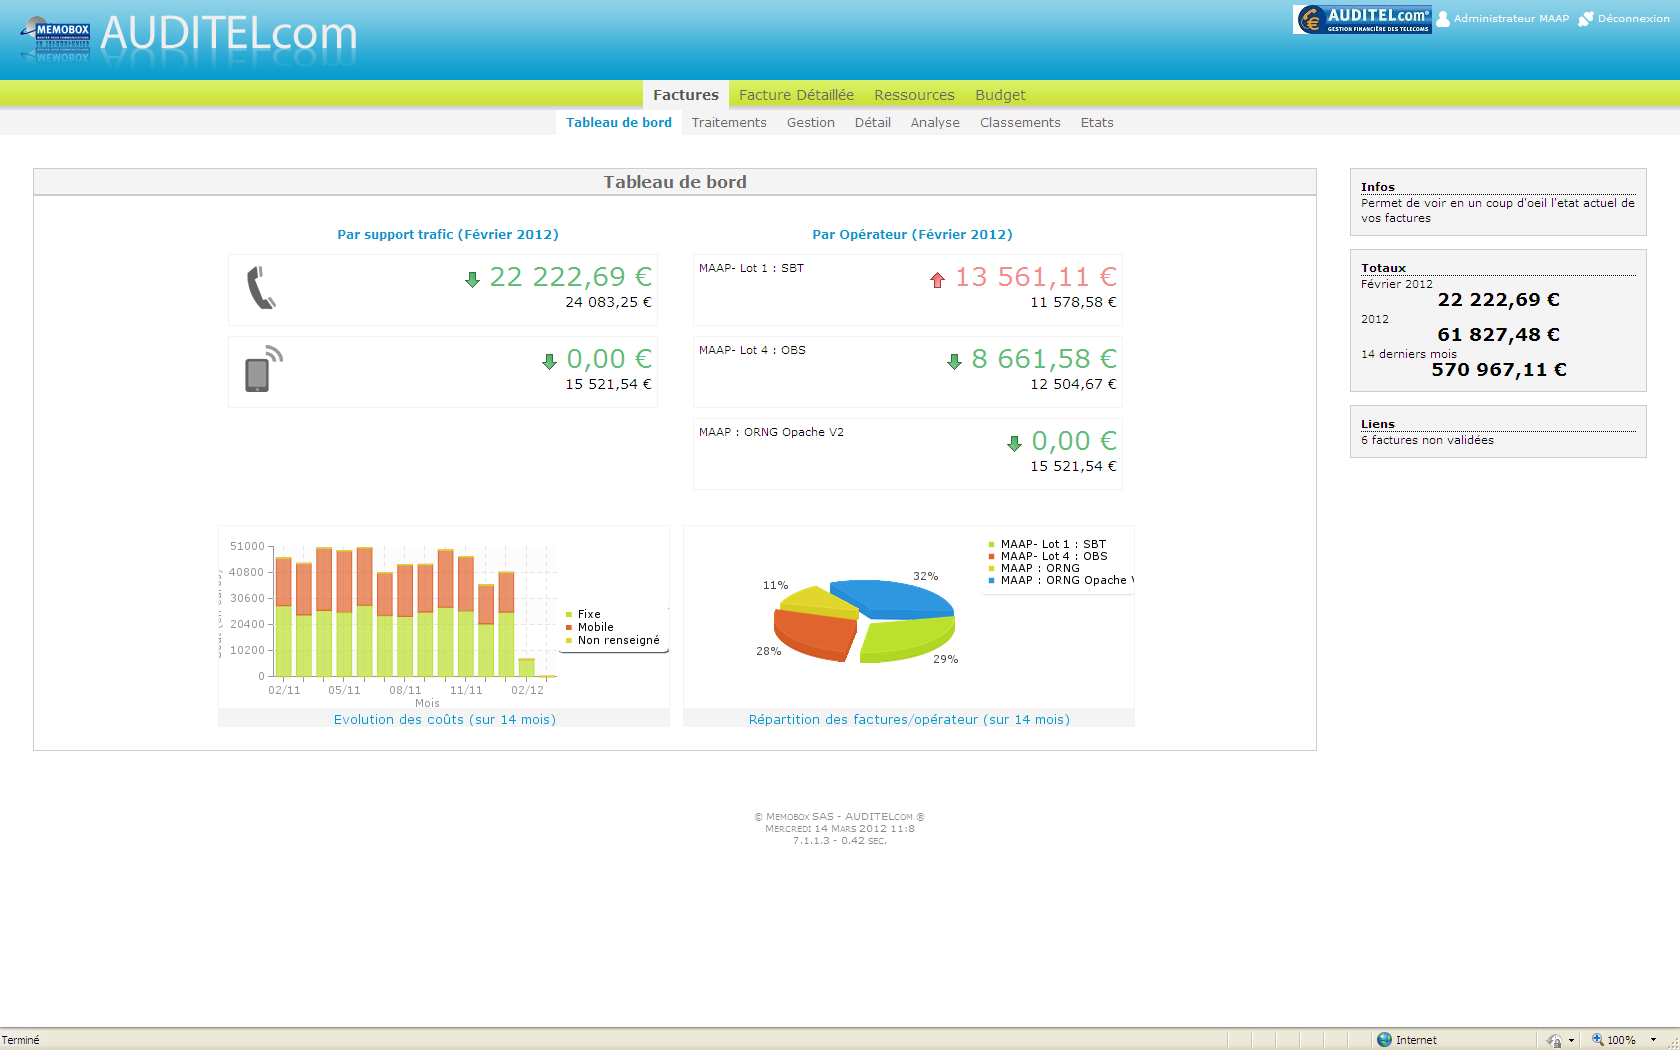
\includegraphics[width=12cm]{images/2-activite/screenAdt.png}
	\caption{\adt{} V7}
\end{figure}
\adt{} est un service en ligne qui, de part son architecture modulaire et sa forte industrialisation, s’adresse aussi bien aux PME\footnote{Petites et Moyennes Entreprises} qu’aux Grands Comptes et Très Grands Comptes.

Fonctionnant en mode SaaS\footnote{Software as a Service}, Cette plateforme peut être installée chez un client ou mutualisée dans les locaux d’un fournisseur de services ou dans ceux de \mbx{}.

Elle assure une qualité irréprochable des données, chose essentielle pour une solution de TEM :
\begin{itemize}
\item Les grilles tarifaires des opérateurs sont en permanence à jour,
\item Les nouveaux PABX et IPBX sont toujours pris en compte,
\item Les nouvelles fonctions statistiques sont mise en ligne,
\item Les nouvelles fonctionnalités sont automatiquement activées.
\end{itemize}


L’offre de service \adt{} délivrée sous forme d’un abonnement, est une solution clé en main permettant de ne pas investir en matériel et logiciel, et de ne pas monopoliser de ressources et de compétences particulières.


\section{Mon rôle}
Lors de mon stage, j'ai participé au développement de \adt{}. J'ai intégré l'équipe de développement composée de \Romain{} et \Denis{}, le système étant en production, il fallait faire attention à n'effectuer aucune régression de l'application,
et effectuer suffisamment de tests avant que mes modifications ne soient apportées sur le serveur de production afin que les clients ne subissent aucune préjudice.

Le développement d'\adt{} fut commencé dans les années 2000 et plusieurs développeurs ont apporté leur contribution, ainsi, on pouvait distinguer différents styles de programmation, certaines portions de code pouvant être vieillissantes.

Lors de mon arrivée, \adt{} était destiné à être multilingue, ainsi il était possible de se connecter en Français, Anglais ou Espagnol. Cependant le système qui permettait à l'application d'être multilingue n'était pas parfait, et rendait difficile la maintenance et
la traduction de l'application. En effet, lorsque nous nous connections pour visualiser l'application en Anglais, la traduction n'était pas effective partout. Ainsi, certaines phrases s'affichaient en français. Cependant la traduction n'allait pas continuer tant que le système n'était pas viable.

Ainsi, mon travail fut d'étudier le système déjà développé, afin d'en analyser les erreurs qui ont été faites pour pouvoir concevoir un nouveau système qui serait beaucoup plus stable et pérenne et rendrait le travail de traduction le plus simple et rapide possible.


\section{\'Etude de l'existant}
\subsection{Le système}
Pour son système de traduction l'application possédait une classe \texttt{TTranslator}, toutes les traductions devaient passer via cette classe à l'aide d'un singleton, la classe \texttt{TTranslator} faisait ensuite des appels à la classe \texttt{TDataLinkAbstract} pour faire le lien
avec la base de données contenant toutes les traductions.
\subsubsection{La table \texttt{RES\_Translations} dite Ancienne Table}
Toutes les traductions étaient stockées dans la table \texttt{RES\_Translations}, ci-dessous sa structure.
\begin{figure}[H]
\centering
% Graphic for TeX using PGF
% Title: C:\Documents and Settings\antoine.deroquemaure\Mes documents\rapportStage\rapport\images\2-activite\bdExistant.dia
% Creator: Dia v0.97.2
% CreationDate: Tue May 29 16:48:55 2012
% For: antoine.deroquemaure
% \usepackage{tikz}
% The following commands are not supported in PSTricks at present
% We define them conditionally, so when they are implemented,
% this pgf file will use them.
\ifx\du\undefined
  \newlength{\du}
\fi
\setlength{\du}{15\unitlength}
\begin{tikzpicture}
\pgftransformxscale{1.000000}
\pgftransformyscale{-1.000000}
\definecolor{dialinecolor}{rgb}{0.000000, 0.000000, 0.000000}
\pgfsetstrokecolor{dialinecolor}
\definecolor{dialinecolor}{rgb}{1.000000, 1.000000, 1.000000}
\pgfsetfillcolor{dialinecolor}
\pgfsetlinewidth{0.030000\du}
\pgfsetdash{}{0pt}
\definecolor{dialinecolor}{rgb}{1.000000, 1.000000, 1.000000}
\pgfsetfillcolor{dialinecolor}
\fill (17.850000\du,14.900000\du)--(17.850000\du,16.300000\du)--(27.205000\du,16.300000\du)--(27.205000\du,14.900000\du)--cycle;
\definecolor{dialinecolor}{rgb}{0.000000, 0.000000, 0.000000}
\pgfsetstrokecolor{dialinecolor}
\draw (17.850000\du,14.900000\du)--(17.850000\du,16.300000\du)--(27.205000\du,16.300000\du)--(27.205000\du,14.900000\du)--cycle;
% setfont left to latex
\definecolor{dialinecolor}{rgb}{0.000000, 0.000000, 0.000000}
\pgfsetstrokecolor{dialinecolor}
\node at (22.527500\du,15.850000\du){\textbf{RES\_Translations}};
\definecolor{dialinecolor}{rgb}{1.000000, 1.000000, 1.000000}
\pgfsetfillcolor{dialinecolor}
\fill (17.850000\du,16.300000\du)--(17.850000\du,21.000000\du)--(27.205000\du,21.000000\du)--(27.205000\du,16.300000\du)--cycle;
\definecolor{dialinecolor}{rgb}{0.000000, 0.000000, 0.000000}
\pgfsetstrokecolor{dialinecolor}
\draw (17.850000\du,16.300000\du)--(17.850000\du,21.000000\du)--(27.205000\du,21.000000\du)--(27.205000\du,16.300000\du)--cycle;
% setfont left to latex
\definecolor{dialinecolor}{rgb}{0.000000, 0.000000, 0.000000}
\pgfsetstrokecolor{dialinecolor}
\node[anchor=west] at (17.965000\du,16.960000\du){\underline{ID\_RES: String}};
% setfont left to latex
\definecolor{dialinecolor}{rgb}{0.000000, 0.000000, 0.000000}
\pgfsetstrokecolor{dialinecolor}
\node[anchor=west] at (17.965000\du,18.20000\du){\underline{Language: Char}};
% setfont left to latex
\definecolor{dialinecolor}{rgb}{0.000000, 0.000000, 0.000000}
\pgfsetstrokecolor{dialinecolor}
\node[anchor=west] at (17.965000\du,19.20000\du){TranslatedText: String};
% setfont left to latex
\definecolor{dialinecolor}{rgb}{0.000000, 0.000000, 0.000000}
\pgfsetstrokecolor{dialinecolor}
\node[anchor=west] at (17.965000\du,20.20000\du){Valide: Boolean};
\end{tikzpicture}

\caption{Table RES\_Translations}
\end{figure}
\begin{description}
	\item[ID\_RES]  Le nom de la constante de traduction.
	\item[Language] La langue de traduction en ISO-639 (fr, en ou es)
	\item[TranslatedText] La valeur de la constante de traduction pour la langue donnée
	\item[Valide] Valide ou non, 1 si la traduction est correcte, 0 sinon.
\end{description}

\subsubsection{La méthode \texttt{getTranslation}}
	La classe \texttt{TTranslator} possédait une méthode \texttt{getTranslation(string, string)}, le premier paramètre était une constante de traduction et le deuxième paramètre, optionnel, correspondait à la langue de traduction.
La constante de traduction permettait de faire le lien avec la base de données, chaque entrée de la base de données était caractérisée par un ID et une Langue.

Ainsi, lorsqu'un développeur souhaitait traduire un texte, il devait connaître la constante de traduction, si celle-ci n'existait pas, il devait ajouter une entrée dans la base de données.

\lstinputlisting[language=PHP, numbers=none, caption=Exemple d'appels de getTranslation]{exemple/2-activite/appelTTranslatorGetTranslation.php}

La langue était optionnelle étant donné que par défaut,  \texttt{TTranslator} utilisait la langue du navigateur, ou la langue demandée lors de la connexion.

\subsection{Avantages et inconvénients du système}
Afin de pouvoir développer un système le plus robuste possible, j'ai analysé l'existant afin d'en tirer les avantages et inconvénients. eux-ci sont disponibles table \ref{table:inconveignantsEtAvantages}.

\begin{table}[H] % TODO
	\centering
	\begin{tabular}{|p{8cm}|p{8cm}|}
		\hline
		\textbf{Avantages} & \textbf{Inconvénients}\\
		\hline
        \begin{minipage}{\linewidth}
        \vspace{10px}
            \begin{itemize}
                \item L'utilisation d'une base de données permet une organisation simple et relationnelle des informations\\
                \item Convention de nommage. Le préfixe LANG\_ pour les ID permet de retrouver facilement une constante dans le code en cas de recherche
            \end{itemize}
        \vspace{10px}
        \end{minipage}
        &
        \begin{minipage}{\linewidth}
        \vspace{10px}
            \begin{itemize}
                \item Duplication de constante, cela vient sûrement des développeurs qui ne trouvant pas une constante, en créaient une autre.
                \item Traduction de certaines variables, comme par exemple 13 derniers mois
                \item Si la constante n'était pas traduite dans la langue demandée, le visiteur verrait un ID, ce qui n'est pas très compréhensible
                \item Recherche, insertion et traduction difficiles.
            \end{itemize}
        \vspace{10px}
        \end{minipage}\\
        \hline
	\end{tabular}
	\caption{Avantages et inconvenients du système}
	\label{table:inconveignantsEtAvantages}
\end{table}

\subsection{Le problème}
Lorsque je suis arrivé, le système de traduction devenait difficile à utiliser. La base de données contenait beaucoup de redondances, par exemple la base contenait 7 ID différents ayant chacun pour valeur \textit{Coût}.\\
\'Egalement elle contenait 378 champs qui n'étaient pas valide, ce nombre assez important rendait le travail de validation beaucoup trop conséquent. Il devenait urgent de trouver un nouveau système.

Ce problème est arrivé en partie à cause des développeurs qui utilisaient le système, il ne pouvait pas facilement savoir si une constante était déjà présente pour ce qu'il voulait faire, ainsi il leurs était plus simple et plus rapide d'en créer une nouvelle,
rapidement la base de données devint incontrôlable. Certains ont également choisis de ne pas créer d'ID, et de mettre leur texte directement dans l'appel de la méthode, cette fois ci ce fut le code du projet qui devint difficile à maîtriser.

\section{Solutions techniques}
	Une fois le système étudié, j'ai réfléchi à des solutions qui pourraient permettre d'avoir un système pérenne, simple à utiliser et qui éviterait les redondances d'informations.
	
	\subsection{Un méta-langage} \label{solRedondance}
	Pour éviter la redondance d'informations, j'ai choisi de créer un méta-langage qui serait utilisé dans la base de données, celui-ci permettrait plusieurs choses :
	\begin{description}
		\item[La concaténation de constante] Pour éviter de traduire toujours les mêmes mots qui reviennent souvent, il paraissait intéressant de pouvoir intégrer un ID de constante dans un texte, ainsi les traducteurs n'auront à traduire qu'une seule fois la dite constante
        \begin{figure}[H]
            \centering
            % Graphic for TeX using PGF
% Title: C:\Documents and Settings\antoine.deroquemaure\Mes documents\stage\rapport\images\2-activite\schemaConst.dia
% Creator: Dia v0.97.2
% CreationDate: Thu Jun 14 10:19:30 2012
% For: antoine.deroquemaure
% \usepackage{tikz}
% The following commands are not supported in PSTricks at present
% We define them conditionally, so when they are implemented,
% this pgf file will use them.
\ifx\du\undefined
  \newlength{\du}
\fi
\setlength{\du}{15\unitlength}
\begin{tikzpicture}
\pgftransformxscale{1.000000}
\pgftransformyscale{-1.000000}
\definecolor{dialinecolor}{rgb}{0.000000, 0.000000, 0.000000}
\pgfsetstrokecolor{dialinecolor}
\definecolor{dialinecolor}{rgb}{1.000000, 1.000000, 1.000000}
\pgfsetfillcolor{dialinecolor}
\pgfsetlinewidth{0.020000\du}
\pgfsetdash{}{0pt}
\pgfsetdash{}{0pt}
\pgfsetmiterjoin
\pgfsetbuttcap
{
\definecolor{dialinecolor}{rgb}{0.000000, 0.000000, 0.000000}
\pgfsetfillcolor{dialinecolor}
% was here!!!
{\pgfsetcornersarced{\pgfpoint{0.000000\du}{0.000000\du}}\definecolor{dialinecolor}{rgb}{0.000000, 0.000000, 0.000000}
\pgfsetstrokecolor{dialinecolor}
\draw (22.400000\du,16.400000\du)--(22.450000\du,16.400000\du)--(24.350000\du,16.400000\du)--(24.400000\du,16.400000\du);
}}
\pgfsetlinewidth{0.020000\du}
\pgfsetdash{}{0pt}
\pgfsetdash{}{0pt}
\pgfsetbuttcap
{
\definecolor{dialinecolor}{rgb}{0.000000, 0.000000, 0.000000}
\pgfsetfillcolor{dialinecolor}
% was here!!!
\definecolor{dialinecolor}{rgb}{0.000000, 0.000000, 0.000000}
\pgfsetstrokecolor{dialinecolor}
\draw (22.400000\du,16.400000\du)--(22.400000\du,15.800000\du);
}
\pgfsetlinewidth{0.020000\du}
\pgfsetdash{}{0pt}
\pgfsetdash{}{0pt}
\pgfsetbuttcap
{
\definecolor{dialinecolor}{rgb}{0.000000, 0.000000, 0.000000}
\pgfsetfillcolor{dialinecolor}
% was here!!!
\definecolor{dialinecolor}{rgb}{0.000000, 0.000000, 0.000000}
\pgfsetstrokecolor{dialinecolor}
\draw (24.400000\du,16.400000\du)--(24.400000\du,15.800000\du);
}
\pgfsetlinewidth{0.020000\du}
\pgfsetdash{}{0pt}
\pgfsetdash{}{0pt}
\pgfsetmiterjoin
\pgfsetbuttcap
{
\definecolor{dialinecolor}{rgb}{0.000000, 0.000000, 0.000000}
\pgfsetfillcolor{dialinecolor}
% was here!!!
{\pgfsetcornersarced{\pgfpoint{0.000000\du}{0.000000\du}}\definecolor{dialinecolor}{rgb}{0.000000, 0.000000, 0.000000}
\pgfsetstrokecolor{dialinecolor}
\draw (9.200000\du,15.000000\du)--(9.210000\du,15.000000\du)--(17.590000\du,15.000000\du)--(17.600000\du,15.000000\du);
}}
\pgfsetlinewidth{0.020000\du}
\pgfsetdash{}{0pt}
\pgfsetdash{}{0pt}
\pgfsetbuttcap
{
\definecolor{dialinecolor}{rgb}{0.000000, 0.000000, 0.000000}
\pgfsetfillcolor{dialinecolor}
% was here!!!
\definecolor{dialinecolor}{rgb}{0.000000, 0.000000, 0.000000}
\pgfsetstrokecolor{dialinecolor}
\draw (9.200000\du,15.000000\du)--(9.200000\du,14.000000\du);
}
\pgfsetlinewidth{0.020000\du}
\pgfsetdash{}{0pt}
\pgfsetdash{}{0pt}
\pgfsetbuttcap
{
\definecolor{dialinecolor}{rgb}{0.000000, 0.000000, 0.000000}
\pgfsetfillcolor{dialinecolor}
% was here!!!
\definecolor{dialinecolor}{rgb}{0.000000, 0.000000, 0.000000}
\pgfsetstrokecolor{dialinecolor}
\draw (17.600000\du,15.000000\du)--(17.600000\du,14.000000\du);
}
\pgfsetlinewidth{0.020000\du}
\pgfsetdash{}{0pt}
\pgfsetdash{}{0pt}
\pgfsetmiterjoin
\pgfsetbuttcap
{
\definecolor{dialinecolor}{rgb}{0.000000, 0.000000, 0.000000}
\pgfsetfillcolor{dialinecolor}
% was here!!!
{\pgfsetcornersarced{\pgfpoint{0.000000\du}{0.000000\du}}\definecolor{dialinecolor}{rgb}{0.000000, 0.000000, 0.000000}
\pgfsetstrokecolor{dialinecolor}
\draw (11.900000\du,14.900000\du)--(11.950000\du,14.900000\du)--(13.850000\du,14.900000\du)--(13.900000\du,14.900000\du);
}}
\pgfsetlinewidth{0.020000\du}
\pgfsetdash{}{0pt}
\pgfsetdash{}{0pt}
\pgfsetbuttcap
{
\definecolor{dialinecolor}{rgb}{0.000000, 0.000000, 0.000000}
\pgfsetfillcolor{dialinecolor}
% was here!!!
\definecolor{dialinecolor}{rgb}{0.000000, 0.000000, 0.000000}
\pgfsetstrokecolor{dialinecolor}
\draw (11.900000\du,14.900000\du)--(11.900000\du,14.400000\du);
}
\pgfsetlinewidth{0.020000\du}
\pgfsetdash{}{0pt}
\pgfsetdash{}{0pt}
\pgfsetbuttcap
{
\definecolor{dialinecolor}{rgb}{0.000000, 0.000000, 0.000000}
\pgfsetfillcolor{dialinecolor}
% was here!!!
\definecolor{dialinecolor}{rgb}{0.000000, 0.000000, 0.000000}
\pgfsetstrokecolor{dialinecolor}
\draw (13.900000\du,14.900000\du)--(13.900000\du,14.400000\du);
}
\pgfsetlinewidth{0.020000\du}
\pgfsetdash{}{0pt}
\pgfsetdash{}{0pt}
\pgfsetmiterjoin
\pgfsetbuttcap
{
\definecolor{dialinecolor}{rgb}{0.000000, 0.000000, 0.000000}
\pgfsetfillcolor{dialinecolor}
% was here!!!
\pgfsetarrowsend{to}
\definecolor{dialinecolor}{rgb}{0.000000, 0.000000, 0.000000}
\pgfsetstrokecolor{dialinecolor}
\pgfpathmoveto{\pgfpoint{23.400000\du}{16.200000\du}}
\pgfpathcurveto{\pgfpoint{23.900000\du}{14.200000\du}}{\pgfpoint{14.500000\du}{13.000000\du}}{\pgfpoint{13.000000\du}{14.400000\du}}
\pgfusepath{stroke}
}
% setfont left to latex
\definecolor{dialinecolor}{rgb}{0.000000, 0.000000, 0.000000}
\pgfsetstrokecolor{dialinecolor}
\node[anchor=west] at (22.600000\du,16.800000\du){Constante};
% setfont left to latex
\definecolor{dialinecolor}{rgb}{0.000000, 0.000000, 0.000000}
\pgfsetstrokecolor{dialinecolor}
\node[anchor=west] at (12.800000\du,15.600000\du){Texte};
\pgfsetlinewidth{0.020000\du}
\pgfsetdash{}{0pt}
\pgfsetdash{}{0pt}
\pgfsetmiterjoin
\pgfsetbuttcap
{
\definecolor{dialinecolor}{rgb}{0.000000, 0.000000, 0.000000}
\pgfsetfillcolor{dialinecolor}
% was here!!!
{\pgfsetcornersarced{\pgfpoint{0.000000\du}{0.000000\du}}\definecolor{dialinecolor}{rgb}{0.000000, 0.000000, 0.000000}
\pgfsetstrokecolor{dialinecolor}
\draw (8.500000\du,18.500000\du)--(19.000000\du,18.500000\du)--(19.000000\du,18.400000\du)--(19.000000\du,18.400000\du);
}}
\pgfsetlinewidth{0.020000\du}
\pgfsetdash{}{0pt}
\pgfsetdash{}{0pt}
\pgfsetbuttcap
{
\definecolor{dialinecolor}{rgb}{0.000000, 0.000000, 0.000000}
\pgfsetfillcolor{dialinecolor}
% was here!!!
\definecolor{dialinecolor}{rgb}{0.000000, 0.000000, 0.000000}
\pgfsetstrokecolor{dialinecolor}
\draw (8.500000\du,18.500000\du)--(8.500000\du,17.500000\du);
}
\pgfsetlinewidth{0.020000\du}
\pgfsetdash{}{0pt}
\pgfsetdash{}{0pt}
\pgfsetbuttcap
{
\definecolor{dialinecolor}{rgb}{0.000000, 0.000000, 0.000000}
\pgfsetfillcolor{dialinecolor}
% was here!!!
\definecolor{dialinecolor}{rgb}{0.000000, 0.000000, 0.000000}
\pgfsetstrokecolor{dialinecolor}
\draw (19.000000\du,18.500000\du)--(19.000000\du,17.500000\du);
}
\pgfsetlinewidth{0.020000\du}
\pgfsetdash{}{0pt}
\pgfsetdash{}{0pt}
\pgfsetmiterjoin
\pgfsetbuttcap
{
\definecolor{dialinecolor}{rgb}{0.000000, 0.000000, 0.000000}
\pgfsetfillcolor{dialinecolor}
% was here!!!
{\pgfsetcornersarced{\pgfpoint{0.000000\du}{0.000000\du}}\definecolor{dialinecolor}{rgb}{0.000000, 0.000000, 0.000000}
\pgfsetstrokecolor{dialinecolor}
\draw (8.600000\du,18.400000\du)--(8.650000\du,18.400000\du)--(10.550000\du,18.400000\du)--(10.600000\du,18.400000\du);
}}
\pgfsetlinewidth{0.020000\du}
\pgfsetdash{}{0pt}
\pgfsetdash{}{0pt}
\pgfsetbuttcap
{
\definecolor{dialinecolor}{rgb}{0.000000, 0.000000, 0.000000}
\pgfsetfillcolor{dialinecolor}
% was here!!!
\definecolor{dialinecolor}{rgb}{0.000000, 0.000000, 0.000000}
\pgfsetstrokecolor{dialinecolor}
\draw (8.600000\du,18.400000\du)--(8.600000\du,17.800000\du);
}
\pgfsetlinewidth{0.020000\du}
\pgfsetdash{}{0pt}
\pgfsetdash{}{0pt}
\pgfsetbuttcap
{
\definecolor{dialinecolor}{rgb}{0.000000, 0.000000, 0.000000}
\pgfsetfillcolor{dialinecolor}
% was here!!!
\definecolor{dialinecolor}{rgb}{0.000000, 0.000000, 0.000000}
\pgfsetstrokecolor{dialinecolor}
\draw (10.600000\du,18.400000\du)--(10.600000\du,17.800000\du);
}
% setfont left to latex
\definecolor{dialinecolor}{rgb}{0.000000, 0.000000, 0.000000}
\pgfsetstrokecolor{dialinecolor}
\node[anchor=west] at (12.400000\du,19.000000\du){Autre texte};
\pgfsetlinewidth{0.020000\du}
\pgfsetdash{}{0pt}
\pgfsetdash{}{0pt}
\pgfsetmiterjoin
\pgfsetbuttcap
{
\definecolor{dialinecolor}{rgb}{0.000000, 0.000000, 0.000000}
\pgfsetfillcolor{dialinecolor}
% was here!!!
\pgfsetarrowsend{to}
\definecolor{dialinecolor}{rgb}{0.000000, 0.000000, 0.000000}
\pgfsetstrokecolor{dialinecolor}
\pgfpathmoveto{\pgfpoint{23.000000\du}{16.200000\du}}
\pgfpathcurveto{\pgfpoint{23.000000\du}{15.700000\du}}{\pgfpoint{13.500000\du}{14.800000\du}}{\pgfpoint{9.500000\du}{17.800000\du}}
\pgfusepath{stroke}
}
\end{tikzpicture}

            \caption{Schéma des constantes}
        \end{figure}
		\item [L'ajout de variables] Il y a souvent des phrases qui reviennent avec seulement une partie du texte qui change, cette partie pourrait être un nombre comme dans 13 derniers mois, mais cela pourrait également être une chaîne de
			caractères comme dans ''appel fixe`` ou ''appel mobile``, en effet, seul le dernier mot change.
		\item[Une gestion du pluriel singulier] L'utilisation de variables numériques va ainsi soulever un problème qui est le singulier ou le pluriel, en effet, comment faisons nous si nous avons 13 lignes fixes ou 1 ligne fixe ?
		Ce méta-langage permettra de choisir comment s'effectue cet accord en fonction de la variable située devant.
	\end{description}
Des exemples de ce méta-langage sont disponible section \ref{exempleMetaLangage} page \pageref{exempleMetaLangage}.

	\subsection{Une application externe ou client lourd} \label{mlanguage}
	La solution précédente semble indispensable afin de prévenir la duplication d'informations, cependant, le problème des développeurs persistera toujours, ils trouveront difficile la recherche, et préféreront créer une nouvelle constante, et nous tomberons dans les mêmes travers que que précédemment.
	
	Ainsi, j'ai choisi de développer une application qui permettrait de palier à ses problèmes. Celle-ci doit être simple d'utilisation, le développeur doit effectuer rapidement ce qu'il veut et le logiciel doit lui faire gagner du temps afin qu'il soit utilisé.

	Cette application permettrait donc les choses suivantes :
	\begin{description}
		\item[Rechercher avec un mot clé ou un ID]  La fonctionnalité principale permettra au développeur de chercher simplement si une constante existe, si celle-ci existe, il pourra copier dans le presse papier l'appel de la méthode afin de lui simplifier
			le travail.
		\item[Ajouter une constante] Si la constante recherchée n'existe pas, il devra être possible d'ajouter une nouvelle constante.
		\item[\'Editer une constante] Il peut arriver qu'une erreur se glisse dans une constante, ainsi il sera possible de la modifier.
		\item[Traduire une constante existante] Quand une constante n'est pas traduite, le développeur, ou un traducteur pourra ajouter la traduction des langues manquantes.
		\item[Basculer une constante de l'ancienne table vers la nouvelle] Étant donné tous les problèmes de la table \texttt{RES\_Translations}, nous avons choisi de créer une nouvelle table \texttt{RES\_dicoLanguage}, cependant, des informations de l'ancienne table sont tout de même
			valables, ainsi il sera possible de demander à basculer un ID de l'ancienne table sur la nouvelle
	\end{description}

	\section{Réalisation des solutions proposées}
		\subsection{La nouvelle classe \texttt{TLanguage}}
		Pour pouvoir effectuer la solution proposée section \ref{solRedondance}, j'ai crée une nouvelle classe PHP, appelée \texttt{TLanguage}. \\
			J'ai choisi de garder les parties fonctionnelles de l'ancien système, c'est-à-dire la détection et le choix de la langue du visiteur, j'ai cependant redéveloppé toute la méthode \texttt{getTranslation}, afin que celle-ci soit capable d'interpréter le meta-langage
		\subsubsection{La base de données, la table \texttt{RES\_dicoLanguage} dite nouvelle table}
			La base de données existante était bien conçue, cependant, mon meta-langage demandait à ajouter un nouveau champ : \texttt{Type}. En effet, nous pouvons inclure dans une phrase un ID, afin de ne pas traduire plusieurs fois la même chose. Il faut faire la différence entre les items, qui sont des mots qui pourront être incluses dans d'autres phrases, et les phrases qui ne doivent jamais être incluses, ceci afin d'éviter
		une éventuelle récursivité pour garder une certaine logique.
	
        \begin{figure}[H]
            \centering
            % Graphic for TeX using PGF
% Title: C:\Documents and Settings\antoine.deroquemaure\Mes documents\stage\rapport\images\2-activite\schemaRecur.dia
% Creator: Dia v0.97.2
% CreationDate: Thu Jun 14 10:30:03 2012
% For: antoine.deroquemaure
% \usepackage{tikz}
% The following commands are not supported in PSTricks at present
% We define them conditionally, so when they are implemented,
% this pgf file will use them.
\ifx\du\undefined
  \newlength{\du}
\fi
\setlength{\du}{15\unitlength}
\begin{tikzpicture}
\pgftransformxscale{1.000000}
\pgftransformyscale{-1.000000}
\definecolor{dialinecolor}{rgb}{0.000000, 0.000000, 0.000000}
\pgfsetstrokecolor{dialinecolor}
\definecolor{dialinecolor}{rgb}{1.000000, 1.000000, 1.000000}
\pgfsetfillcolor{dialinecolor}
\pgfsetlinewidth{0.020000\du}
\pgfsetdash{}{0pt}
\pgfsetdash{}{0pt}
\pgfsetmiterjoin
\pgfsetbuttcap
{
\definecolor{dialinecolor}{rgb}{0.000000, 0.000000, 0.000000}
\pgfsetfillcolor{dialinecolor}
% was here!!!
{\pgfsetcornersarced{\pgfpoint{0.000000\du}{0.000000\du}}\definecolor{dialinecolor}{rgb}{0.000000, 0.000000, 0.000000}
\pgfsetstrokecolor{dialinecolor}
\draw (9.200000\du,15.000000\du)--(9.210000\du,15.000000\du)--(17.590000\du,15.000000\du)--(17.600000\du,15.000000\du);
}}
\pgfsetlinewidth{0.020000\du}
\pgfsetdash{}{0pt}
\pgfsetdash{}{0pt}
\pgfsetbuttcap
{
\definecolor{dialinecolor}{rgb}{0.000000, 0.000000, 0.000000}
\pgfsetfillcolor{dialinecolor}
% was here!!!
\definecolor{dialinecolor}{rgb}{0.000000, 0.000000, 0.000000}
\pgfsetstrokecolor{dialinecolor}
\draw (9.200000\du,15.000000\du)--(9.200000\du,14.000000\du);
}
\pgfsetlinewidth{0.020000\du}
\pgfsetdash{}{0pt}
\pgfsetdash{}{0pt}
\pgfsetbuttcap
{
\definecolor{dialinecolor}{rgb}{0.000000, 0.000000, 0.000000}
\pgfsetfillcolor{dialinecolor}
% was here!!!
\definecolor{dialinecolor}{rgb}{0.000000, 0.000000, 0.000000}
\pgfsetstrokecolor{dialinecolor}
\draw (17.600000\du,15.000000\du)--(17.600000\du,14.000000\du);
}
\pgfsetlinewidth{0.020000\du}
\pgfsetdash{}{0pt}
\pgfsetdash{}{0pt}
\pgfsetmiterjoin
\pgfsetbuttcap
{
\definecolor{dialinecolor}{rgb}{0.000000, 0.000000, 0.000000}
\pgfsetfillcolor{dialinecolor}
% was here!!!
{\pgfsetcornersarced{\pgfpoint{0.000000\du}{0.000000\du}}\definecolor{dialinecolor}{rgb}{0.000000, 0.000000, 0.000000}
\pgfsetstrokecolor{dialinecolor}
\draw (11.900000\du,14.900000\du)--(11.950000\du,14.900000\du)--(13.850000\du,14.900000\du)--(13.900000\du,14.900000\du);
}}
\pgfsetlinewidth{0.020000\du}
\pgfsetdash{}{0pt}
\pgfsetdash{}{0pt}
\pgfsetbuttcap
{
\definecolor{dialinecolor}{rgb}{0.000000, 0.000000, 0.000000}
\pgfsetfillcolor{dialinecolor}
% was here!!!
\definecolor{dialinecolor}{rgb}{0.000000, 0.000000, 0.000000}
\pgfsetstrokecolor{dialinecolor}
\draw (11.900000\du,14.900000\du)--(11.900000\du,14.400000\du);
}
\pgfsetlinewidth{0.020000\du}
\pgfsetdash{}{0pt}
\pgfsetdash{}{0pt}
\pgfsetbuttcap
{
\definecolor{dialinecolor}{rgb}{0.000000, 0.000000, 0.000000}
\pgfsetfillcolor{dialinecolor}
% was here!!!
\definecolor{dialinecolor}{rgb}{0.000000, 0.000000, 0.000000}
\pgfsetstrokecolor{dialinecolor}
\draw (13.900000\du,14.900000\du)--(13.900000\du,14.400000\du);
}
\pgfsetlinewidth{0.020000\du}
\pgfsetdash{}{0pt}
\pgfsetdash{}{0pt}
\pgfsetmiterjoin
\pgfsetbuttcap
{
\definecolor{dialinecolor}{rgb}{0.000000, 0.000000, 0.000000}
\pgfsetfillcolor{dialinecolor}
% was here!!!
\pgfsetarrowsend{to}
\definecolor{dialinecolor}{rgb}{0.000000, 0.000000, 0.000000}
\pgfsetstrokecolor{dialinecolor}
\pgfpathmoveto{\pgfpoint{15.000000\du}{12.400000\du}}
\pgfpathcurveto{\pgfpoint{15.200000\du}{12.800000\du}}{\pgfpoint{13.000000\du}{12.400000\du}}{\pgfpoint{12.800000\du}{14.400000\du}}
\pgfusepath{stroke}
}
\pgfsetlinewidth{0.020000\du}
\pgfsetdash{}{0pt}
\pgfsetdash{}{0pt}
\pgfsetmiterjoin
\pgfsetbuttcap
{
\definecolor{dialinecolor}{rgb}{0.000000, 0.000000, 0.000000}
\pgfsetfillcolor{dialinecolor}
% was here!!!
{\pgfsetcornersarced{\pgfpoint{0.000000\du}{0.000000\du}}\definecolor{dialinecolor}{rgb}{0.000000, 0.000000, 0.000000}
\pgfsetstrokecolor{dialinecolor}
\draw (10.000000\du,12.400000\du)--(17.500000\du,12.400000\du)--(17.500000\du,12.100000\du)--(17.500000\du,12.100000\du);
}}
\pgfsetlinewidth{0.020000\du}
\pgfsetdash{}{0pt}
\pgfsetdash{}{0pt}
\pgfsetbuttcap
{
\definecolor{dialinecolor}{rgb}{0.000000, 0.000000, 0.000000}
\pgfsetfillcolor{dialinecolor}
% was here!!!
\definecolor{dialinecolor}{rgb}{0.000000, 0.000000, 0.000000}
\pgfsetstrokecolor{dialinecolor}
\draw (10.000000\du,12.400000\du)--(10.000000\du,11.400000\du);
}
\pgfsetlinewidth{0.020000\du}
\pgfsetdash{}{0pt}
\pgfsetdash{}{0pt}
\pgfsetbuttcap
{
\definecolor{dialinecolor}{rgb}{0.000000, 0.000000, 0.000000}
\pgfsetfillcolor{dialinecolor}
% was here!!!
\definecolor{dialinecolor}{rgb}{0.000000, 0.000000, 0.000000}
\pgfsetstrokecolor{dialinecolor}
\draw (17.500000\du,12.300000\du)--(17.500000\du,11.300000\du);
}
\pgfsetlinewidth{0.020000\du}
\pgfsetdash{}{0pt}
\pgfsetdash{}{0pt}
\pgfsetmiterjoin
\pgfsetbuttcap
{
\definecolor{dialinecolor}{rgb}{0.000000, 0.000000, 0.000000}
\pgfsetfillcolor{dialinecolor}
% was here!!!
{\pgfsetcornersarced{\pgfpoint{0.000000\du}{0.000000\du}}\definecolor{dialinecolor}{rgb}{0.000000, 0.000000, 0.000000}
\pgfsetstrokecolor{dialinecolor}
\draw (10.100000\du,12.300000\du)--(10.150000\du,12.300000\du)--(12.050000\du,12.300000\du)--(12.100000\du,12.300000\du);
}}
\pgfsetlinewidth{0.020000\du}
\pgfsetdash{}{0pt}
\pgfsetdash{}{0pt}
\pgfsetbuttcap
{
\definecolor{dialinecolor}{rgb}{0.000000, 0.000000, 0.000000}
\pgfsetfillcolor{dialinecolor}
% was here!!!
\definecolor{dialinecolor}{rgb}{0.000000, 0.000000, 0.000000}
\pgfsetstrokecolor{dialinecolor}
\draw (10.100000\du,12.300000\du)--(10.100000\du,11.700000\du);
}
\pgfsetlinewidth{0.020000\du}
\pgfsetdash{}{0pt}
\pgfsetdash{}{0pt}
\pgfsetbuttcap
{
\definecolor{dialinecolor}{rgb}{0.000000, 0.000000, 0.000000}
\pgfsetfillcolor{dialinecolor}
% was here!!!
\definecolor{dialinecolor}{rgb}{0.000000, 0.000000, 0.000000}
\pgfsetstrokecolor{dialinecolor}
\draw (12.100000\du,12.300000\du)--(12.100000\du,11.700000\du);
}
\pgfsetlinewidth{0.020000\du}
\pgfsetdash{}{0pt}
\pgfsetdash{}{0pt}
\pgfsetmiterjoin
\pgfsetbuttcap
{
\definecolor{dialinecolor}{rgb}{0.000000, 0.000000, 0.000000}
\pgfsetfillcolor{dialinecolor}
% was here!!!
{\pgfsetcornersarced{\pgfpoint{0.000000\du}{0.000000\du}}\definecolor{dialinecolor}{rgb}{0.000000, 0.000000, 0.000000}
\pgfsetstrokecolor{dialinecolor}
\draw (9.600000\du,10.200000\du)--(9.610000\du,10.200000\du)--(17.990000\du,10.200000\du)--(18.000000\du,10.200000\du);
}}
\pgfsetlinewidth{0.020000\du}
\pgfsetdash{}{0pt}
\pgfsetdash{}{0pt}
\pgfsetbuttcap
{
\definecolor{dialinecolor}{rgb}{0.000000, 0.000000, 0.000000}
\pgfsetfillcolor{dialinecolor}
% was here!!!
\definecolor{dialinecolor}{rgb}{0.000000, 0.000000, 0.000000}
\pgfsetstrokecolor{dialinecolor}
\draw (9.600000\du,10.200000\du)--(9.600000\du,9.200000\du);
}
\pgfsetlinewidth{0.020000\du}
\pgfsetdash{}{0pt}
\pgfsetdash{}{0pt}
\pgfsetbuttcap
{
\definecolor{dialinecolor}{rgb}{0.000000, 0.000000, 0.000000}
\pgfsetfillcolor{dialinecolor}
% was here!!!
\definecolor{dialinecolor}{rgb}{0.000000, 0.000000, 0.000000}
\pgfsetstrokecolor{dialinecolor}
\draw (18.000000\du,10.200000\du)--(18.000000\du,9.200000\du);
}
\pgfsetlinewidth{0.020000\du}
\pgfsetdash{}{0pt}
\pgfsetdash{}{0pt}
\pgfsetmiterjoin
\pgfsetbuttcap
{
\definecolor{dialinecolor}{rgb}{0.000000, 0.000000, 0.000000}
\pgfsetfillcolor{dialinecolor}
% was here!!!
{\pgfsetcornersarced{\pgfpoint{0.000000\du}{0.000000\du}}\definecolor{dialinecolor}{rgb}{0.000000, 0.000000, 0.000000}
\pgfsetstrokecolor{dialinecolor}
\draw (12.300000\du,10.100000\du)--(12.350000\du,10.100000\du)--(14.250000\du,10.100000\du)--(14.300000\du,10.100000\du);
}}
\pgfsetlinewidth{0.020000\du}
\pgfsetdash{}{0pt}
\pgfsetdash{}{0pt}
\pgfsetbuttcap
{
\definecolor{dialinecolor}{rgb}{0.000000, 0.000000, 0.000000}
\pgfsetfillcolor{dialinecolor}
% was here!!!
\definecolor{dialinecolor}{rgb}{0.000000, 0.000000, 0.000000}
\pgfsetstrokecolor{dialinecolor}
\draw (12.300000\du,10.100000\du)--(12.300000\du,9.600000\du);
}
\pgfsetlinewidth{0.020000\du}
\pgfsetdash{}{0pt}
\pgfsetdash{}{0pt}
\pgfsetbuttcap
{
\definecolor{dialinecolor}{rgb}{0.000000, 0.000000, 0.000000}
\pgfsetfillcolor{dialinecolor}
% was here!!!
\definecolor{dialinecolor}{rgb}{0.000000, 0.000000, 0.000000}
\pgfsetstrokecolor{dialinecolor}
\draw (14.300000\du,10.100000\du)--(14.300000\du,9.600000\du);
}
\pgfsetlinewidth{0.020000\du}
\pgfsetdash{}{0pt}
\pgfsetdash{}{0pt}
\pgfsetmiterjoin
\pgfsetbuttcap
{
\definecolor{dialinecolor}{rgb}{0.000000, 0.000000, 0.000000}
\pgfsetfillcolor{dialinecolor}
% was here!!!
\pgfsetarrowsend{to}
\definecolor{dialinecolor}{rgb}{0.000000, 0.000000, 0.000000}
\pgfsetstrokecolor{dialinecolor}
\pgfpathmoveto{\pgfpoint{9.600000\du}{10.200000\du}}
\pgfpathcurveto{\pgfpoint{9.800000\du}{10.600000\du}}{\pgfpoint{11.200000\du}{10.000000\du}}{\pgfpoint{11.000000\du}{12.000000\du}}
\pgfusepath{stroke}
}
\pgfsetlinewidth{0.020000\du}
\pgfsetdash{}{0pt}
\pgfsetdash{}{0pt}
\pgfsetmiterjoin
\pgfsetbuttcap
{
\definecolor{dialinecolor}{rgb}{0.000000, 0.000000, 0.000000}
\pgfsetfillcolor{dialinecolor}
% was here!!!
{\pgfsetcornersarced{\pgfpoint{0.000000\du}{0.000000\du}}\definecolor{dialinecolor}{rgb}{0.000000, 0.000000, 0.000000}
\pgfsetstrokecolor{dialinecolor}
\draw (12.000000\du,8.200000\du)--(12.050000\du,8.200000\du)--(13.950000\du,8.200000\du)--(14.000000\du,8.200000\du);
}}
\pgfsetlinewidth{0.020000\du}
\pgfsetdash{}{0pt}
\pgfsetdash{}{0pt}
\pgfsetbuttcap
{
\definecolor{dialinecolor}{rgb}{0.000000, 0.000000, 0.000000}
\pgfsetfillcolor{dialinecolor}
% was here!!!
\definecolor{dialinecolor}{rgb}{0.000000, 0.000000, 0.000000}
\pgfsetstrokecolor{dialinecolor}
\draw (12.000000\du,8.200000\du)--(12.000000\du,7.700000\du);
}
\pgfsetlinewidth{0.020000\du}
\pgfsetdash{}{0pt}
\pgfsetdash{}{0pt}
\pgfsetbuttcap
{
\definecolor{dialinecolor}{rgb}{0.000000, 0.000000, 0.000000}
\pgfsetfillcolor{dialinecolor}
% was here!!!
\definecolor{dialinecolor}{rgb}{0.000000, 0.000000, 0.000000}
\pgfsetstrokecolor{dialinecolor}
\draw (14.000000\du,8.200000\du)--(14.000000\du,7.700000\du);
}
\pgfsetlinewidth{0.020000\du}
\pgfsetdash{}{0pt}
\pgfsetdash{}{0pt}
\pgfsetmiterjoin
\pgfsetbuttcap
{
\definecolor{dialinecolor}{rgb}{0.000000, 0.000000, 0.000000}
\pgfsetfillcolor{dialinecolor}
% was here!!!
\pgfsetarrowsend{to}
\definecolor{dialinecolor}{rgb}{0.000000, 0.000000, 0.000000}
\pgfsetstrokecolor{dialinecolor}
\pgfpathmoveto{\pgfpoint{12.800000\du}{8.000000\du}}
\pgfpathcurveto{\pgfpoint{13.000000\du}{8.400000\du}}{\pgfpoint{14.000000\du}{7.800000\du}}{\pgfpoint{13.800000\du}{9.800000\du}}
\pgfusepath{stroke}
}
\end{tikzpicture}

            \caption{Le problème qui sera évité avec les items et les phrases.}
        \end{figure}
		Ainsi, la nouvelle table devient donc:

		\begin{figure}[H] %%%%%% TODO %%%%%% NOUVELLE BASE ET MODIFICATION SUITE (short, normal, long)
			\centering
			% Graphic for TeX using PGF
% Title: C:\Documents and Settings\antoine.deroquemaure\Mes documents\stage\rapport\images\2-activite\bdNouvelle.dia
% Creator: Dia v0.97.2
% CreationDate: Thu Jun 14 10:37:26 2012
% For: antoine.deroquemaure
% \usepackage{tikz}
% The following commands are not supported in PSTricks at present
% We define them conditionally, so when they are implemented,
% this pgf file will use them.
\ifx\du\undefined
  \newlength{\du}
\fi
\setlength{\du}{15\unitlength}
\begin{tikzpicture}
\pgftransformxscale{1.000000}
\pgftransformyscale{-1.000000}
\definecolor{dialinecolor}{rgb}{0.000000, 0.000000, 0.000000}
\pgfsetstrokecolor{dialinecolor}
\definecolor{dialinecolor}{rgb}{1.000000, 1.000000, 1.000000}
\pgfsetfillcolor{dialinecolor}
\pgfsetlinewidth{0.030000\du}
\pgfsetdash{}{0pt}
\definecolor{dialinecolor}{rgb}{1.000000, 1.000000, 1.000000}
\pgfsetfillcolor{dialinecolor}
\fill (17.850000\du,14.900000\du)--(17.850000\du,16.300000\du)--(27.205000\du,16.300000\du)--(27.205000\du,14.900000\du)--cycle;
\definecolor{dialinecolor}{rgb}{0.000000, 0.000000, 0.000000}
\pgfsetstrokecolor{dialinecolor}
\draw (17.850000\du,14.900000\du)--(17.850000\du,16.300000\du)--(27.205000\du,16.300000\du)--(27.205000\du,14.900000\du)--cycle;
% setfont left to latex
\definecolor{dialinecolor}{rgb}{0.000000, 0.000000, 0.000000}
\pgfsetstrokecolor{dialinecolor}
\node at (22.527500\du,15.850000\du){RES\_Translations};
\definecolor{dialinecolor}{rgb}{1.000000, 1.000000, 1.000000}
\pgfsetfillcolor{dialinecolor}
\fill (17.850000\du,16.300000\du)--(17.850000\du,20.500000\du)--(27.205000\du,20.500000\du)--(27.205000\du,16.300000\du)--cycle;
\definecolor{dialinecolor}{rgb}{0.000000, 0.000000, 0.000000}
\pgfsetstrokecolor{dialinecolor}
\draw (17.850000\du,16.300000\du)--(17.850000\du,20.500000\du)--(27.205000\du,20.500000\du)--(27.205000\du,16.300000\du)--cycle;
% setfont left to latex
\definecolor{dialinecolor}{rgb}{0.000000, 0.000000, 0.000000}
\pgfsetstrokecolor{dialinecolor}
\node[anchor=west] at (17.965000\du,17.00000\du){\underline{ID\_RES: String}};
% setfont left to latex
\definecolor{dialinecolor}{rgb}{0.000000, 0.000000, 0.000000}
\pgfsetstrokecolor{dialinecolor}
\node[anchor=west] at (17.965000\du,18.000000\du){\underline{Language: Char}};
% setfont left to latex
\definecolor{dialinecolor}{rgb}{0.000000, 0.000000, 0.000000}
\pgfsetstrokecolor{dialinecolor}
\node[anchor=west] at (17.965000\du,19.00000\du){Type};
% setfont left to latex
\definecolor{dialinecolor}{rgb}{0.000000, 0.000000, 0.000000}
\pgfsetstrokecolor{dialinecolor}
\node[anchor=west] at (17.965000\du,20.00000\du){TranslatedText: String};
% setfont left to latex
\definecolor{dialinecolor}{rgb}{0.000000, 0.000000, 0.000000}
\pgfsetstrokecolor{dialinecolor}
\node[anchor=west] at (17.965000\du,21.00000\du){Valide: Boolean};
\pgfsetlinewidth{0.020000\du}
\pgfsetdash{}{0pt}
\definecolor{dialinecolor}{rgb}{1.000000, 1.000000, 1.000000}
\pgfsetfillcolor{dialinecolor}
\fill (28.600000\du,17.600000\du)--(36.520000\du,17.600000\du)--(37.120000\du,18.200000\du)--(37.120000\du,19.300000\du)--(28.600000\du,19.300000\du)--cycle;
\definecolor{dialinecolor}{rgb}{0.000000, 0.000000, 0.000000}
\pgfsetstrokecolor{dialinecolor}
\draw (28.600000\du,17.600000\du)--(36.520000\du,17.600000\du)--(37.120000\du,18.200000\du)--(37.120000\du,19.300000\du)--(28.600000\du,19.300000\du)--cycle;
\pgfsetlinewidth{0.010000\du}
\definecolor{dialinecolor}{rgb}{0.000000, 0.000000, 0.000000}
\pgfsetstrokecolor{dialinecolor}
\draw (36.520000\du,17.600000\du)--(36.520000\du,18.200000\du)--(37.120000\du,18.200000\du);
% setfont left to latex
\definecolor{dialinecolor}{rgb}{0.000000, 0.000000, 0.000000}
\pgfsetstrokecolor{dialinecolor}
\node[anchor=west] at (28.910000\du,18.742500\du){ITEM ou PHRA};
\pgfsetlinewidth{0.020000\du}
\pgfsetdash{{1.000000\du}{1.000000\du}}{0\du}
\pgfsetdash{{0.500000\du}{0.500000\du}}{0\du}
\pgfsetbuttcap
{
\definecolor{dialinecolor}{rgb}{0.000000, 0.000000, 0.000000}
\pgfsetfillcolor{dialinecolor}
% was here!!!
\definecolor{dialinecolor}{rgb}{0.000000, 0.000000, 0.000000}
\pgfsetstrokecolor{dialinecolor}
\draw (28.600000\du,18.450000\du)--(19.972315\du,19.007748\du);
}
\end{tikzpicture}

			\caption{Table \texttt{RES\_dicoLanguage}}
		\end{figure}

		\subsubsection{La méthode \texttt{getTranslation}}\label{exempleMetaLangage}
			J'ai redéveloppé intégralement cette méthode afin de pouvoir y intégrer un parseur qui interpréte le méta-langage.
			Ainsi, une fois développé il est possible, comme expliqué section \ref{solRedondance} de :
			\begin{description}
		\item[Concaténer des constantes]  Pour cela, il suffit au développeur d'ajouter dans la valeur de traduction [NOM\_ID] avec \texttt{NOM\_ID} ayant pour valeur l'ID d'une constante de traduction. Les crochets seront ainsi remplacés par la constante en question.

			Si la constante n'a pas été traduite pour la langue du visiteur, celle-ci sera affichée en Français.
%			\exemple{
			\begin{exemple}{}
			\begin{table}[H]
				\centering
				\rowcolors{2}{grisclair}{grisfonce}
				\begin{tabular}{|c|p{5.2cm}|c|}
					\hline
					ID\_RES & TranslatedText & Type\_RES \\
					TRANS\_GENERAL\_DATA &Données [TRANS\_GENERAL] & PHRA \\
					TRANS\_GENERALES  & Générales & ITEM \\
					\hline
				\end{tabular}\vspace{10px}
                \caption[Exemple de constante]{Exemple de constante -- Base de données}
				\lstinputlisting[language=PHP, numbers=none, caption=Exemple de constante -- Code]{exemple/2-activite/exempleConstantes.php}
				
				\texttt{Données Générales}
			\end{table}
			\captionExemple{Utilisation des constantes}
			\end{exemple}
		\item [Ajouter des variables] Il est également possible d'ajouter des variables dans une valeur, ainsi, dans le champ de la base de données, le développeur doit mettre <variable>, \textit{variable} pouvant être remplacée par ce qu'il veut. Cela
			permet de donner un nom à sa variable pour que les personnes trouvant la constante comprennent à quoi correspond celle-ci. Lors de l'appel de la méthode \texttt{getTranslation} le développeur fera passer la liste des arguments
			nécessaires au bon fonctionnement de la traduction.
			\begin{exemple}{Utilisation des variables}
			\begin{table}[H]
				\centering
				\rowcolors{2}{grisclair}{grisfonce}
				\begin{tabular}{|c|p{5.2cm}|c|}
					\hline
					ID\_RES & TranslatedText & Type\_RES \\
					TRANS\_PBX\_NO\_LINES & <nbPBX> PBX sans ligne ni poste& PHRA\\
					\hline
				\end{tabular}\vspace{10px}
                \caption[Exemple de variables]{Exemple de variables -- Base de données}				\lstinputlisting[language=PHP, numbers=none, caption=Exemple de variables -- Code]{exemple/2-activite/exempleVariables.php}

				\texttt{4 PBX sans ligne ni poste}
			\end{table}
			\captionExemple{Utilisation des variables}
			\end{exemple}
% Exemple
\newpage
		\item[Gérer le pluriel ou le singulier]  Si le développeur à mis des variables qui attendent un nombre, il doit signaler les accords éventuels qui suivent la variable avec la syntaxe \texttt{(sing|plur)}.
			\begin{exemple}{}
			\begin{table}[H]
				\centering
				\rowcolors{2}{grisclair}{grisfonce}
				\begin{tabular}{|c|p{5.2cm}|c|}
					\hline
					ID\_RES & TranslatedText & Type\_RES \\
					TRANS\_NB\_RINGINGS& <nbSonneries> sonneri(e|es)& PHRA \\
					\hline
				\end{tabular}\vspace{10px}
                \caption[Exemple avec du pluriel/singulier]{Exemple avec du pluriel/singulier -- Base de données}
				\lstinputlisting[language=PHP, numbers=none, caption=Exemple avec du pluriel/singulier -- Code]{exemple/2-activite/exemplePlurOrSing.php}

				\texttt{15 sonneries}
			\end{table}
			\captionExemple{Utilisation du pluriel et du singulier}
			\end{exemple}
			\end{description}
    \subsection{Le client lourd : MemoLanguage}
        Une fois le nouveau moteur de traduction développé, il me fallait concevoir un outil de traduction aidant le développeur comme expliqué section \ref{mlanguage} page \pageref{mlanguage}. \\
        Cet outil fut baptisé \mlanguage{}, à mon départ, il en était à sa version 0.9.
        \subsubsection{Méthode Agile}
            Afin d'avoir un client lourd qui soit le plus adapté aux besoins possibles, nous avons choisis une méthode Agile, par itération successives. Ainsi, une fois qu'une première version de \mlanguage{} était finit, j'ai mis le logiciel en production, l'utilisation du logiciel a permis de rapidement ajouter de nouvelles fonctionnalités afin de satisfaire au maximum les besoins de l'entreprise.

            Le logiciel a été développé en 5 iterations successives, les résultats qui suivent sont les résultats obtenus après 4 itérations. La 5ème est disponible section \ref{iteration} afin que vous puissiez voir un exemple d'itération.
        \subsubsection{Technologies choisies}

       \begin{wrapfigure}{r}{2.5cm}
            
\includegraphics[width=2.5cm]{images/2-activite/air.jpg}
        \end{wrapfigure}
        Afin d'avoir l'outil le plus pratique possible, celui-ci devait être installé en natif chez chacun des développeurs, en effet il était plus pratique pour les développeurs d'avoir une application dans la barre des tâches. Une page web n'aurait pas été pratique, en effet, le développeur aurait dû changer d'onglet régulièrement, alors qu'une application native peut être mis dans un coin, ou réduite au besoin du développeur.

         Ainsi, la technologie choisis fut \texttt{Adobe Air}\footnote{Adobe Integrated Runtime}, c'est une machine virtuelle multi-plateforme qui s'exécute sur le système d'exploitation.

        Il est ainsi possible d'utiliser des technologies web pour créer un client natif, ce qui permet d'avoir la puissance d'une application native avec la souplesse des technologies web.
        \newpage
       \begin{wrapfigure}{l}{2cm}
            
\includegraphics[width=2.0cm]{images/2-activite/javascript.jpg}
        \end{wrapfigure}
        Pour effectuer des recherches sur un serveur distant, avoir une bonne ergonomie et ne pas avoir à recharger la page continuellement, j'ai choisi d'utiliser du JavaScript pour développer le client,
        sa puissance me permettant d'interroger le serveur.

        Je l'ai couplé avec du XHTML\footnote{eXtensible HyperText Markup Language} et du CSS\footnote{Cascading Style Sheets} pour l'affichage et la mise en forme.

        C'est donc avec la combinaison de ces technologies que j'ai utilisé l'AJAX\footnote{\textbf{A}synchronous \textbf{Ja}vascript and \textbf{X}ML}\\

     \begin{wrapfigure}[4]{r}{2cm}
           
\includegraphics[width=2cm]{images/2-activite/mysql.jpg}
     \end{wrapfigure}
        Il fallait cependant également développer un serveur qui ferait le lien entre le client \texttt{Adobe Air} et la base de données, cette base de données étant celle d'\adt{}, c'est une base de données MySQL, ce qui permet d'avoir une base facilement interfaçable avec Apache et PHP tout en gardant de bonnes performances.\\

     \begin{wrapfigure}[2]{l}{2cm}\vspace{-5px}
           
\includegraphics[width=2cm]{images/2-activite/php.png}
      \end{wrapfigure}
        Le serveur sera donc codé en PHP Orienté Objet. Cela permettera d'avoir le maximum de puissance, mais également un code propre, organisé et réutilisable. \\~\\~\\~\\~~

    Ainsi, nous avons une architecture client serveur, cette architecture est disponible figure \ref{fig:archiClientServeur}.
    \begin{figure}[H]
        \centering
        % Graphic for TeX using PGF
% Title: C:\Documents and Settings\antoine.deroquemaure\Mes documents\stage\rapport\images\2-activite\archiClientServeur.dia
% Creator: Dia v0.97.2
% CreationDate: Thu Jun 14 13:46:45 2012
% For: antoine.deroquemaure
% \usepackage{tikz}
% The following commands are not supported in PSTricks at present
% We define them conditionally, so when they are implemented,
% this pgf file will use them.
\ifx\du\undefined
  \newlength{\du}
\fi
\setlength{\du}{15\unitlength}
\begin{tikzpicture}
\pgftransformxscale{1.000000}
\pgftransformyscale{-1.000000}
\definecolor{dialinecolor}{rgb}{0.000000, 0.000000, 0.000000}
\pgfsetstrokecolor{dialinecolor}
\definecolor{dialinecolor}{rgb}{1.000000, 1.000000, 1.000000}
\pgfsetfillcolor{dialinecolor}
\pgfsetlinewidth{0.020000\du}
\pgfsetdash{}{0pt}
\pgfsetdash{}{0pt}
\pgfsetbuttcap
\pgfsetmiterjoin
\pgfsetlinewidth{0.016000\du}
\pgfsetbuttcap
\pgfsetmiterjoin
\pgfsetdash{}{0pt}
\definecolor{dialinecolor}{rgb}{0.701961, 0.701961, 0.701961}
\pgfsetfillcolor{dialinecolor}
\fill (16.695191\du,5.400000\du)--(16.695191\du,8.843899\du)--(18.171148\du,8.843899\du)--(18.171148\du,5.400000\du)--cycle;
\definecolor{dialinecolor}{rgb}{0.000000, 0.000000, 0.000000}
\pgfsetstrokecolor{dialinecolor}
\draw (16.695191\du,5.400000\du)--(16.695191\du,8.843899\du)--(18.171148\du,8.843899\du)--(18.171148\du,5.400000\du)--cycle;
\pgfsetlinewidth{0.002000\du}
\pgfsetbuttcap
\pgfsetmiterjoin
\pgfsetdash{}{0pt}
\definecolor{dialinecolor}{rgb}{0.000000, 0.000000, 0.000000}
\pgfsetstrokecolor{dialinecolor}
\draw (16.842787\du,5.606634\du)--(16.842787\du,6.000222\du)--(18.023553\du,6.000222\du)--(18.023553\du,5.606634\du)--cycle;
\pgfsetbuttcap
\pgfsetmiterjoin
\pgfsetdash{}{0pt}
\definecolor{dialinecolor}{rgb}{0.000000, 0.000000, 0.000000}
\pgfsetstrokecolor{dialinecolor}
\draw (16.842787\du,6.000222\du)--(16.842787\du,6.393811\du)--(18.023553\du,6.393811\du)--(18.023553\du,6.000222\du)--cycle;
\pgfsetbuttcap
\pgfsetmiterjoin
\pgfsetdash{}{0pt}
\definecolor{dialinecolor}{rgb}{0.000000, 0.000000, 0.000000}
\pgfsetstrokecolor{dialinecolor}
\draw (16.842787\du,6.393811\du)--(16.842787\du,6.787399\du)--(18.023553\du,6.787399\du)--(18.023553\du,6.393811\du)--cycle;
\pgfsetbuttcap
\pgfsetmiterjoin
\pgfsetdash{}{0pt}
\definecolor{dialinecolor}{rgb}{0.000000, 0.000000, 0.000000}
\pgfsetstrokecolor{dialinecolor}
\draw (16.842787\du,6.787399\du)--(16.842787\du,7.180988\du)--(18.023553\du,7.180988\du)--(18.023553\du,6.787399\du)--cycle;
\pgfsetbuttcap
\pgfsetmiterjoin
\pgfsetdash{}{0pt}
\definecolor{dialinecolor}{rgb}{0.000000, 0.000000, 0.000000}
\pgfsetstrokecolor{dialinecolor}
\draw (16.842787\du,7.259706\du)--(16.842787\du,7.495859\du)--(17.580765\du,7.495859\du)--(17.580765\du,7.259706\du)--cycle;
\pgfsetbuttcap
\pgfsetmiterjoin
\pgfsetdash{}{0pt}
\definecolor{dialinecolor}{rgb}{0.000000, 1.000000, 0.000000}
\pgfsetfillcolor{dialinecolor}
\pgfpathellipse{\pgfpoint{17.949755\du}{7.299064\du}}{\pgfpoint{0.051658\du}{0\du}}{\pgfpoint{0\du}{0.051658\du}}
\pgfusepath{fill}
\definecolor{dialinecolor}{rgb}{0.000000, 0.000000, 0.000000}
\pgfsetstrokecolor{dialinecolor}
\pgfpathellipse{\pgfpoint{17.949755\du}{7.299064\du}}{\pgfpoint{0.051658\du}{0\du}}{\pgfpoint{0\du}{0.051658\du}}
\pgfusepath{stroke}
\pgfsetbuttcap
\pgfsetmiterjoin
\pgfsetdash{}{0pt}
\definecolor{dialinecolor}{rgb}{1.000000, 1.000000, 0.000000}
\pgfsetfillcolor{dialinecolor}
\pgfpathellipse{\pgfpoint{17.949755\du}{7.456500\du}}{\pgfpoint{0.051658\du}{0\du}}{\pgfpoint{0\du}{0.051658\du}}
\pgfusepath{fill}
\definecolor{dialinecolor}{rgb}{0.000000, 0.000000, 0.000000}
\pgfsetstrokecolor{dialinecolor}
\pgfpathellipse{\pgfpoint{17.949755\du}{7.456500\du}}{\pgfpoint{0.051658\du}{0\du}}{\pgfpoint{0\du}{0.051658\du}}
\pgfusepath{stroke}
\pgfsetbuttcap
\pgfsetmiterjoin
\pgfsetdash{}{0pt}
\definecolor{dialinecolor}{rgb}{1.000000, 1.000000, 1.000000}
\pgfsetfillcolor{dialinecolor}
\fill (17.654563\du,7.338423\du)--(17.654563\du,7.495859\du)--(17.831678\du,7.495859\du)--(17.831678\du,7.338423\du)--cycle;
\definecolor{dialinecolor}{rgb}{0.000000, 0.000000, 0.000000}
\pgfsetstrokecolor{dialinecolor}
\draw (17.654563\du,7.338423\du)--(17.654563\du,7.495859\du)--(17.831678\du,7.495859\du)--(17.831678\du,7.338423\du)--cycle;
\pgfsetbuttcap
\pgfsetmiterjoin
\pgfsetdash{}{0pt}
\definecolor{dialinecolor}{rgb}{0.000000, 0.000000, 0.000000}
\pgfsetstrokecolor{dialinecolor}
\pgfpathmoveto{\pgfpoint{16.941184\du}{7.810730\du}}
\pgfpathlineto{\pgfpoint{16.941184\du}{8.671704\du}}
\pgfusepath{stroke}
\pgfsetbuttcap
\pgfsetmiterjoin
\pgfsetdash{}{0pt}
\definecolor{dialinecolor}{rgb}{0.000000, 0.000000, 0.000000}
\pgfsetstrokecolor{dialinecolor}
\pgfpathmoveto{\pgfpoint{17.187177\du}{7.810730\du}}
\pgfpathlineto{\pgfpoint{17.187177\du}{8.671704\du}}
\pgfusepath{stroke}
\pgfsetbuttcap
\pgfsetmiterjoin
\pgfsetdash{}{0pt}
\definecolor{dialinecolor}{rgb}{0.000000, 0.000000, 0.000000}
\pgfsetstrokecolor{dialinecolor}
\pgfpathmoveto{\pgfpoint{17.433170\du}{7.810730\du}}
\pgfpathlineto{\pgfpoint{17.433170\du}{8.671704\du}}
\pgfusepath{stroke}
\pgfsetbuttcap
\pgfsetmiterjoin
\pgfsetdash{}{0pt}
\definecolor{dialinecolor}{rgb}{0.000000, 0.000000, 0.000000}
\pgfsetstrokecolor{dialinecolor}
\pgfpathmoveto{\pgfpoint{17.679163\du}{7.810730\du}}
\pgfpathlineto{\pgfpoint{17.679163\du}{8.671704\du}}
\pgfusepath{stroke}
\pgfsetbuttcap
\pgfsetmiterjoin
\pgfsetdash{}{0pt}
\definecolor{dialinecolor}{rgb}{0.000000, 0.000000, 0.000000}
\pgfsetstrokecolor{dialinecolor}
\pgfpathmoveto{\pgfpoint{17.925155\du}{7.810730\du}}
\pgfpathlineto{\pgfpoint{17.925155\du}{8.671704\du}}
\pgfusepath{stroke}
\pgfsetbuttcap
\pgfsetmiterjoin
\pgfsetdash{}{0pt}
\definecolor{dialinecolor}{rgb}{0.000000, 0.000000, 0.000000}
\pgfsetstrokecolor{dialinecolor}
\pgfpathmoveto{\pgfpoint{18.171148\du}{7.810730\du}}
\pgfpathlineto{\pgfpoint{18.171148\du}{8.671704\du}}
\pgfusepath{stroke}
\pgfsetbuttcap
\pgfsetmiterjoin
\pgfsetdash{}{0pt}
\definecolor{dialinecolor}{rgb}{0.600000, 0.600000, 0.600000}
\pgfsetfillcolor{dialinecolor}
\fill (16.400000\du,9.139091\du)--(16.695191\du,8.548708\du)--(16.695191\du,8.843899\du)--(18.171148\du,8.843899\du)--(18.171148\du,8.548708\du)--(18.564737\du,9.139091\du)--cycle;
\definecolor{dialinecolor}{rgb}{0.000000, 0.000000, 0.000000}
\pgfsetstrokecolor{dialinecolor}
\draw (16.400000\du,9.139091\du)--(16.695191\du,8.548708\du)--(16.695191\du,8.843899\du)--(18.171148\du,8.843899\du)--(18.171148\du,8.548708\du)--(18.564737\du,9.139091\du)--cycle;
% setfont left to latex
\definecolor{dialinecolor}{rgb}{0.000000, 0.000000, 0.000000}
\pgfsetstrokecolor{dialinecolor}
\node at (17.482368\du,9.887488\du){};
\pgfsetlinewidth{0.020000\du}
\pgfsetdash{}{0pt}
\pgfsetdash{}{0pt}
\pgfsetbuttcap
\pgfsetmiterjoin
\pgfsetlinewidth{0.020000\du}
\pgfsetbuttcap
\pgfsetmiterjoin
\pgfsetdash{}{0pt}
\definecolor{dialinecolor}{rgb}{1.000000, 1.000000, 1.000000}
\pgfsetfillcolor{dialinecolor}
\fill (25.500000\du,6.356215\du)--(25.500000\du,8.493505\du)--(27.922262\du,8.493505\du)--(27.922262\du,6.356215\du)--cycle;
\pgfsetbuttcap
\pgfsetmiterjoin
\pgfsetdash{}{0pt}
\definecolor{dialinecolor}{rgb}{1.000000, 1.000000, 1.000000}
\pgfsetfillcolor{dialinecolor}
\pgfpathellipse{\pgfpoint{26.711131\du}{8.493505\du}}{\pgfpoint{1.211131\du}{0\du}}{\pgfpoint{0\du}{0.356215\du}}
\pgfusepath{fill}
\pgfsetbuttcap
\pgfsetmiterjoin
\pgfsetdash{}{0pt}
\definecolor{dialinecolor}{rgb}{1.000000, 1.000000, 1.000000}
\pgfsetfillcolor{dialinecolor}
\pgfpathellipse{\pgfpoint{26.711131\du}{6.356215\du}}{\pgfpoint{1.211131\du}{0\du}}{\pgfpoint{0\du}{0.356215\du}}
\pgfusepath{fill}
\definecolor{dialinecolor}{rgb}{0.000000, 0.000000, 0.000000}
\pgfsetstrokecolor{dialinecolor}
\pgfpathellipse{\pgfpoint{26.711131\du}{6.356215\du}}{\pgfpoint{1.211131\du}{0\du}}{\pgfpoint{0\du}{0.356215\du}}
\pgfusepath{stroke}
\pgfsetbuttcap
\pgfsetmiterjoin
\pgfsetdash{}{0pt}
\definecolor{dialinecolor}{rgb}{0.000000, 0.000000, 0.000000}
\pgfsetstrokecolor{dialinecolor}
\pgfpathmoveto{\pgfpoint{27.922262\du}{6.356215\du}}
\pgfpathlineto{\pgfpoint{27.922262\du}{8.493505\du}}
\pgfpathcurveto{\pgfpoint{27.922262\du}{8.690237\du}}{\pgfpoint{27.380020\du}{8.849720\du}}{\pgfpoint{26.711131\du}{8.849720\du}}
\pgfpathcurveto{\pgfpoint{26.042242\du}{8.849720\du}}{\pgfpoint{25.500000\du}{8.690237\du}}{\pgfpoint{25.500000\du}{8.493505\du}}
\pgfpathlineto{\pgfpoint{25.500000\du}{6.356215\du}}
\pgfusepath{stroke}
% setfont left to latex
\definecolor{dialinecolor}{rgb}{0.000000, 0.000000, 0.000000}
\pgfsetstrokecolor{dialinecolor}
\node at (26.711131\du,9.499720\du){};
\pgfsetlinewidth{0.020000\du}
\pgfsetdash{}{0pt}
\pgfsetdash{}{0pt}
\pgfsetbuttcap
{
\definecolor{dialinecolor}{rgb}{0.000000, 0.000000, 0.000000}
\pgfsetfillcolor{dialinecolor}
% was here!!!
\pgfsetarrowsend{to}
\definecolor{dialinecolor}{rgb}{0.000000, 0.000000, 0.000000}
\pgfsetstrokecolor{dialinecolor}
\draw (18.400000\du,7.000000\du)--(25.400000\du,7.000000\du);
}
\pgfsetlinewidth{0.020000\du}
\pgfsetdash{}{0pt}
\pgfsetdash{}{0pt}
\pgfsetbuttcap
{
\definecolor{dialinecolor}{rgb}{0.000000, 0.000000, 0.000000}
\pgfsetfillcolor{dialinecolor}
% was here!!!
\pgfsetarrowsstart{to}
\definecolor{dialinecolor}{rgb}{0.000000, 0.000000, 0.000000}
\pgfsetstrokecolor{dialinecolor}
\draw (18.500000\du,8.000000\du)--(25.500000\du,8.000000\du);
}
\pgfsetlinewidth{0.020000\du}
\pgfsetdash{}{0pt}
\pgfsetdash{}{0pt}
\pgfsetbuttcap
\pgfsetmiterjoin
\pgfsetlinewidth{0.010000\du}
\pgfsetbuttcap
\pgfsetmiterjoin
\pgfsetdash{}{0pt}
\definecolor{dialinecolor}{rgb}{0.701961, 0.701961, 0.701961}
\pgfsetfillcolor{dialinecolor}
\fill (16.300000\du,12.900000\du)--(16.300000\du,14.716525\du)--(18.722034\du,14.716525\du)--(18.722034\du,12.900000\du)--cycle;
\definecolor{dialinecolor}{rgb}{0.000000, 0.000000, 0.000000}
\pgfsetstrokecolor{dialinecolor}
\draw (16.300000\du,12.900000\du)--(16.300000\du,14.716525\du)--(18.722034\du,14.716525\du)--(18.722034\du,12.900000\du)--cycle;
\pgfsetlinewidth{0.020000\du}
\pgfsetbuttcap
\pgfsetmiterjoin
\pgfsetdash{}{0pt}
\definecolor{dialinecolor}{rgb}{0.000000, 0.000000, 0.000000}
\pgfsetfillcolor{dialinecolor}
\fill (16.562387\du,13.162387\du)--(16.562387\du,14.413771\du)--(18.459647\du,14.413771\du)--(18.459647\du,13.162387\du)--cycle;
\pgfsetlinewidth{0.010000\du}
\pgfsetbuttcap
\pgfsetmiterjoin
\pgfsetdash{}{0pt}
\definecolor{dialinecolor}{rgb}{0.701961, 0.701961, 0.701961}
\pgfsetfillcolor{dialinecolor}
\fill (16.627984\du,14.716525\du)--(17.874322\du,14.716525\du)--(17.874322\du,14.999096\du)--(16.693581\du,14.999096\du)--cycle;
\definecolor{dialinecolor}{rgb}{0.000000, 0.000000, 0.000000}
\pgfsetstrokecolor{dialinecolor}
\draw (16.627984\du,14.716525\du)--(17.874322\du,14.716525\du)--(17.874322\du,14.999096\du)--(16.693581\du,14.999096\du)--cycle;
\pgfsetbuttcap
\pgfsetmiterjoin
\pgfsetdash{}{0pt}
\definecolor{dialinecolor}{rgb}{0.701961, 0.701961, 0.701961}
\pgfsetfillcolor{dialinecolor}
\fill (17.874322\du,14.716525\du)--(18.394050\du,14.716525\du)--(18.328453\du,14.999096\du)--(17.874322\du,14.999096\du)--cycle;
\definecolor{dialinecolor}{rgb}{0.000000, 0.000000, 0.000000}
\pgfsetstrokecolor{dialinecolor}
\draw (17.874322\du,14.716525\du)--(18.394050\du,14.716525\du)--(18.328453\du,14.999096\du)--(17.874322\du,14.999096\du)--cycle;
\pgfsetlinewidth{0.005000\du}
\pgfsetbuttcap
\pgfsetmiterjoin
\pgfsetdash{}{0pt}
\definecolor{dialinecolor}{rgb}{1.000000, 1.000000, 1.000000}
\pgfsetfillcolor{dialinecolor}
\fill (17.959093\du,14.801297\du)--(17.959093\du,14.914325\du)--(18.072121\du,14.914325\du)--(18.072121\du,14.801297\du)--cycle;
\definecolor{dialinecolor}{rgb}{0.000000, 0.000000, 0.000000}
\pgfsetstrokecolor{dialinecolor}
\draw (17.959093\du,14.801297\du)--(17.959093\du,14.914325\du)--(18.072121\du,14.914325\du)--(18.072121\du,14.801297\du)--cycle;
\pgfsetlinewidth{0.010000\du}
\pgfsetbuttcap
\pgfsetmiterjoin
\pgfsetdash{}{0pt}
\definecolor{dialinecolor}{rgb}{0.701961, 0.701961, 0.701961}
\pgfsetfillcolor{dialinecolor}
\fill (17.268814\du,14.999096\du)--(17.753220\du,14.999096\du)--(17.753220\du,15.140381\du)--(17.995424\du,15.140381\du)--(17.995424\du,15.281667\du)--(17.026610\du,15.281667\du)--(17.026610\du,15.140381\du)--(17.268814\du,15.140381\du)--cycle;
\definecolor{dialinecolor}{rgb}{0.000000, 0.000000, 0.000000}
\pgfsetstrokecolor{dialinecolor}
\draw (17.268814\du,14.999096\du)--(17.753220\du,14.999096\du)--(17.753220\du,15.140381\du)--(17.995424\du,15.140381\du)--(17.995424\du,15.281667\du)--(17.026610\du,15.281667\du)--(17.026610\du,15.140381\du)--(17.268814\du,15.140381\du)--cycle;
% setfont left to latex
\definecolor{dialinecolor}{rgb}{0.000000, 0.000000, 0.000000}
\pgfsetstrokecolor{dialinecolor}
\node at (17.511017\du,16.012401\du){};
\pgfsetlinewidth{0.020000\du}
\pgfsetdash{}{0pt}
\pgfsetdash{}{0pt}
\pgfsetbuttcap
{
\definecolor{dialinecolor}{rgb}{0.000000, 0.000000, 0.000000}
\pgfsetfillcolor{dialinecolor}
% was here!!!
\pgfsetarrowsend{to}
\definecolor{dialinecolor}{rgb}{0.000000, 0.000000, 0.000000}
\pgfsetstrokecolor{dialinecolor}
\draw (17.200000\du,12.600000\du)--(17.200000\du,9.200000\du);
}
\pgfsetlinewidth{0.020000\du}
\pgfsetdash{}{0pt}
\pgfsetdash{}{0pt}
\pgfsetbuttcap
{
\definecolor{dialinecolor}{rgb}{0.000000, 0.000000, 0.000000}
\pgfsetfillcolor{dialinecolor}
% was here!!!
\pgfsetarrowsstart{to}
\definecolor{dialinecolor}{rgb}{0.000000, 0.000000, 0.000000}
\pgfsetstrokecolor{dialinecolor}
\draw (17.800000\du,12.600000\du)--(17.800000\du,9.200000\du);
}
% setfont left to latex
\definecolor{dialinecolor}{rgb}{0.000000, 0.000000, 0.000000}
\pgfsetstrokecolor{dialinecolor}
\node[anchor=west] at (13.800000\du,11.500000\du){Requête};
% setfont left to latex
\definecolor{dialinecolor}{rgb}{0.000000, 0.000000, 0.000000}
\pgfsetstrokecolor{dialinecolor}
\node[anchor=west] at (17.900000\du,11.500000\du){Réponse};
% setfont left to latex
\definecolor{dialinecolor}{rgb}{0.000000, 0.000000, 0.000000}
\pgfsetstrokecolor{dialinecolor}
\node[anchor=west] at (20.000000\du,8.600000\du){Réponse};
% setfont left to latex
\definecolor{dialinecolor}{rgb}{0.000000, 0.000000, 0.000000}
\pgfsetstrokecolor{dialinecolor}
\node[anchor=west] at (19.40828\du,6.499598\du){Interrogation};
% setfont left to latex
\definecolor{dialinecolor}{rgb}{0.000000, 0.000000, 0.000000}
\pgfsetstrokecolor{dialinecolor}
\node[anchor=west] at (15.300000\du,4.700000\du){\bsc{SERVEUR}};
% setfont left to latex
\definecolor{dialinecolor}{rgb}{0.000000, 0.000000, 0.000000}
\pgfsetstrokecolor{dialinecolor}
\node[anchor=west] at (23.000000\du,9.500000\du){\bsc{BASE DE DONN\'EE}};
% setfont left to latex
\definecolor{dialinecolor}{rgb}{0.000000, 0.000000, 0.000000}
\pgfsetstrokecolor{dialinecolor}
\node[anchor=west] at (15.700000\du,16.000000\du){\bsc{CLIENT}};
\end{tikzpicture}

        \caption{Architecture client -- serveur}
        \label{fig:archiClientServeur}
    \end{figure}
        \subsubsection{Développement du serveur}
            Le serveur est destiné à être appelé via le JavaScript, donc juste avec l'URL, ainsi toutes les variables seront dans l'URL.

        J'ai donc choisi une architecture où toutes les requêtes s'articulent autour d'un fichier index.php, avec plusieurs variables en URL.
        \begin{figure}[H]
            \hspace{-35px};
            % Graphic for TeX using PGF
% Title: C:\Documents and Settings\antoine.deroquemaure\Mes documents\stage\rapport\images\2-activite\DiagrammeClassServer.dia
% Creator: Dia v0.97.2
% CreationDate: Mon Jun 11 18:51:01 2012
% For: antoine.deroquemaure
% \usepackage{tikz}
% The following commands are not supported in PSTricks at present
% We define them conditionally, so when they are implemented,
% this pgf file will use them.
\ifx\du\undefined
  \newlength{\du}
\fi
\setlength{\du}{15\unitlength}
\begin{tikzpicture}
\pgftransformxscale{1.000000}
\pgftransformyscale{-1.000000}
\definecolor{dialinecolor}{rgb}{0.000000, 0.000000, 0.000000}
\pgfsetstrokecolor{dialinecolor}
\definecolor{dialinecolor}{rgb}{1.000000, 1.000000, 1.000000}
\pgfsetfillcolor{dialinecolor}
\pgfsetlinewidth{0.020000\du}
\pgfsetdash{}{0pt}
\definecolor{dialinecolor}{rgb}{1.000000, 1.000000, 1.000000}
\pgfsetfillcolor{dialinecolor}
\fill (-12.000000\du,0.000000\du)--(-12.000000\du,1.400000\du)--(-7.265000\du,1.400000\du)--(-7.265000\du,0.000000\du)--cycle;
\definecolor{dialinecolor}{rgb}{0.000000, 0.000000, 0.000000}
\pgfsetstrokecolor{dialinecolor}
\draw (-12.000000\du,0.000000\du)--(-12.000000\du,1.400000\du)--(-7.265000\du,1.400000\du)--(-7.265000\du,0.000000\du)--cycle;
% setfont left to latex
\definecolor{dialinecolor}{rgb}{0.000000, 0.000000, 0.000000}
\pgfsetstrokecolor{dialinecolor}
\node at (-9.632500\du,0.950000\du){\textit{Page}};
\definecolor{dialinecolor}{rgb}{1.000000, 1.000000, 1.000000}
\pgfsetfillcolor{dialinecolor}
\fill (-12.000000\du,1.400000\du)--(-12.000000\du,2.400000\du)--(-7.265000\du,2.400000\du)--(-7.265000\du,1.400000\du)--cycle;
\definecolor{dialinecolor}{rgb}{0.000000, 0.000000, 0.000000}
\pgfsetstrokecolor{dialinecolor}
\draw (-12.000000\du,1.400000\du)--(-12.000000\du,2.400000\du)--(-7.265000\du,2.400000\du)--(-7.265000\du,1.400000\du)--cycle;
% setfont left to latex
\definecolor{dialinecolor}{rgb}{0.000000, 0.000000, 0.000000}
\pgfsetstrokecolor{dialinecolor}
\node[anchor=west] at (-11.890000\du,2.060000\du){\#text};
\definecolor{dialinecolor}{rgb}{1.000000, 1.000000, 1.000000}
\pgfsetfillcolor{dialinecolor}
\fill (-12.000000\du,2.400000\du)--(-12.000000\du,4.200000\du)--(-7.265000\du,4.200000\du)--(-7.265000\du,2.400000\du)--cycle;
\definecolor{dialinecolor}{rgb}{0.000000, 0.000000, 0.000000}
\pgfsetstrokecolor{dialinecolor}
\draw (-12.000000\du,2.400000\du)--(-12.000000\du,4.200000\du)--(-7.265000\du,4.200000\du)--(-7.265000\du,2.400000\du)--cycle;
% setfont left to latex
\definecolor{dialinecolor}{rgb}{0.000000, 0.000000, 0.000000}
\pgfsetstrokecolor{dialinecolor}
\node[anchor=west] at (-11.890000\du,3.060000\du){+display()};
% setfont left to latex
\definecolor{dialinecolor}{rgb}{0.000000, 0.000000, 0.000000}
\pgfsetstrokecolor{dialinecolor}
\node[anchor=west] at (-11.890000\du,3.860000\du){\textit{\#initText()}};
\pgfsetlinewidth{0.020000\du}
\pgfsetdash{}{0pt}
\definecolor{dialinecolor}{rgb}{1.000000, 1.000000, 1.000000}
\pgfsetfillcolor{dialinecolor}
\fill (-30.000000\du,14.000000\du)--(-30.000000\du,15.400000\du)--(-25.232500\du,15.400000\du)--(-25.232500\du,14.000000\du)--cycle;
\definecolor{dialinecolor}{rgb}{0.000000, 0.000000, 0.000000}
\pgfsetstrokecolor{dialinecolor}
\draw (-30.000000\du,14.000000\du)--(-30.000000\du,15.400000\du)--(-25.232500\du,15.400000\du)--(-25.232500\du,14.000000\du)--cycle;
% setfont left to latex
\definecolor{dialinecolor}{rgb}{0.000000, 0.000000, 0.000000}
\pgfsetstrokecolor{dialinecolor}
\node at (-27.616250\du,14.950000\du){\textbf{PageSelect}};
\definecolor{dialinecolor}{rgb}{1.000000, 1.000000, 1.000000}
\pgfsetfillcolor{dialinecolor}
\fill (-30.000000\du,15.400000\du)--(-30.000000\du,20.400000\du)--(-25.232500\du,20.400000\du)--(-25.232500\du,15.400000\du)--cycle;
\definecolor{dialinecolor}{rgb}{0.000000, 0.000000, 0.000000}
\pgfsetstrokecolor{dialinecolor}
\draw (-30.000000\du,15.400000\du)--(-30.000000\du,20.400000\du)--(-25.232500\du,20.400000\du)--(-25.232500\du,15.400000\du)--cycle;
% setfont left to latex
\definecolor{dialinecolor}{rgb}{0.000000, 0.000000, 0.000000}
\pgfsetstrokecolor{dialinecolor}
\node[anchor=west] at (-29.890000\du,16.060000\du){-keyword};
% setfont left to latex
\definecolor{dialinecolor}{rgb}{0.000000, 0.000000, 0.000000}
\pgfsetstrokecolor{dialinecolor}
\node[anchor=west] at (-29.890000\du,16.860000\du){-typeSearch};
% setfont left to latex
\definecolor{dialinecolor}{rgb}{0.000000, 0.000000, 0.000000}
\pgfsetstrokecolor{dialinecolor}
\node[anchor=west] at (-29.890000\du,17.660000\du){-langResult};
% setfont left to latex
\definecolor{dialinecolor}{rgb}{0.000000, 0.000000, 0.000000}
\pgfsetstrokecolor{dialinecolor}
\node[anchor=west] at (-29.890000\du,18.460000\du){-langSearch};
% setfont left to latex
\definecolor{dialinecolor}{rgb}{0.000000, 0.000000, 0.000000}
\pgfsetstrokecolor{dialinecolor}
\node[anchor=west] at (-29.890000\du,19.260000\du){-valide};
% setfont left to latex
\definecolor{dialinecolor}{rgb}{0.000000, 0.000000, 0.000000}
\pgfsetstrokecolor{dialinecolor}
\node[anchor=west] at (-29.890000\du,20.060000\du){-table};
\definecolor{dialinecolor}{rgb}{1.000000, 1.000000, 1.000000}
\pgfsetfillcolor{dialinecolor}
\fill (-30.000000\du,20.400000\du)--(-30.000000\du,21.400000\du)--(-25.232500\du,21.400000\du)--(-25.232500\du,20.400000\du)--cycle;
\definecolor{dialinecolor}{rgb}{0.000000, 0.000000, 0.000000}
\pgfsetstrokecolor{dialinecolor}
\draw (-30.000000\du,20.400000\du)--(-30.000000\du,21.400000\du)--(-25.232500\du,21.400000\du)--(-25.232500\du,20.400000\du)--cycle;
% setfont left to latex
\definecolor{dialinecolor}{rgb}{0.000000, 0.000000, 0.000000}
\pgfsetstrokecolor{dialinecolor}
\node[anchor=west] at (-29.890000\du,21.060000\du){ initText()};
\pgfsetlinewidth{0.020000\du}
\pgfsetdash{}{0pt}
\definecolor{dialinecolor}{rgb}{1.000000, 1.000000, 1.000000}
\pgfsetfillcolor{dialinecolor}
\fill (-24.000000\du,14.000000\du)--(-24.000000\du,15.400000\du)--(-19.187500\du,15.400000\du)--(-19.187500\du,14.000000\du)--cycle;
\definecolor{dialinecolor}{rgb}{0.000000, 0.000000, 0.000000}
\pgfsetstrokecolor{dialinecolor}
\draw (-24.000000\du,14.000000\du)--(-24.000000\du,15.400000\du)--(-19.187500\du,15.400000\du)--(-19.187500\du,14.000000\du)--cycle;
% setfont left to latex
\definecolor{dialinecolor}{rgb}{0.000000, 0.000000, 0.000000}
\pgfsetstrokecolor{dialinecolor}
\node at (-21.593750\du,14.950000\du){\textbf{PageDelete}};
\definecolor{dialinecolor}{rgb}{1.000000, 1.000000, 1.000000}
\pgfsetfillcolor{dialinecolor}
\fill (-24.000000\du,15.400000\du)--(-24.000000\du,16.400000\du)--(-19.187500\du,16.400000\du)--(-19.187500\du,15.400000\du)--cycle;
\definecolor{dialinecolor}{rgb}{0.000000, 0.000000, 0.000000}
\pgfsetstrokecolor{dialinecolor}
\draw (-24.000000\du,15.400000\du)--(-24.000000\du,16.400000\du)--(-19.187500\du,16.400000\du)--(-19.187500\du,15.400000\du)--cycle;
% setfont left to latex
\definecolor{dialinecolor}{rgb}{0.000000, 0.000000, 0.000000}
\pgfsetstrokecolor{dialinecolor}
\node[anchor=west] at (-23.890000\du,16.060000\du){-id};
\definecolor{dialinecolor}{rgb}{1.000000, 1.000000, 1.000000}
\pgfsetfillcolor{dialinecolor}
\fill (-24.000000\du,16.400000\du)--(-24.000000\du,17.400000\du)--(-19.187500\du,17.400000\du)--(-19.187500\du,16.400000\du)--cycle;
\definecolor{dialinecolor}{rgb}{0.000000, 0.000000, 0.000000}
\pgfsetstrokecolor{dialinecolor}
\draw (-24.000000\du,16.400000\du)--(-24.000000\du,17.400000\du)--(-19.187500\du,17.400000\du)--(-19.187500\du,16.400000\du)--cycle;
% setfont left to latex
\definecolor{dialinecolor}{rgb}{0.000000, 0.000000, 0.000000}
\pgfsetstrokecolor{dialinecolor}
\node[anchor=west] at (-23.890000\du,17.060000\du){ initText()};
\pgfsetlinewidth{0.020000\du}
\pgfsetdash{}{0pt}
\definecolor{dialinecolor}{rgb}{1.000000, 1.000000, 1.000000}
\pgfsetfillcolor{dialinecolor}
\fill (-18.000000\du,14.000000\du)--(-18.000000\du,15.400000\du)--(-11.725000\du,15.400000\du)--(-11.725000\du,14.000000\du)--cycle;
\definecolor{dialinecolor}{rgb}{0.000000, 0.000000, 0.000000}
\pgfsetstrokecolor{dialinecolor}
\draw (-18.000000\du,14.000000\du)--(-18.000000\du,15.400000\du)--(-11.725000\du,15.400000\du)--(-11.725000\du,14.000000\du)--cycle;
% setfont left to latex
\definecolor{dialinecolor}{rgb}{0.000000, 0.000000, 0.000000}
\pgfsetstrokecolor{dialinecolor}
\node at (-14.862500\du,14.950000\du){\textbf{PageUpdate}};
\definecolor{dialinecolor}{rgb}{1.000000, 1.000000, 1.000000}
\pgfsetfillcolor{dialinecolor}
\fill (-18.000000\du,15.400000\du)--(-18.000000\du,19.600000\du)--(-11.725000\du,19.600000\du)--(-11.725000\du,15.400000\du)--cycle;
\definecolor{dialinecolor}{rgb}{0.000000, 0.000000, 0.000000}
\pgfsetstrokecolor{dialinecolor}
\draw (-18.000000\du,15.400000\du)--(-18.000000\du,19.600000\du)--(-11.725000\du,19.600000\du)--(-11.725000\du,15.400000\du)--cycle;
% setfont left to latex
\definecolor{dialinecolor}{rgb}{0.000000, 0.000000, 0.000000}
\pgfsetstrokecolor{dialinecolor}
\node[anchor=west] at (-17.890000\du,16.060000\du){-id};
% setfont left to latex
\definecolor{dialinecolor}{rgb}{0.000000, 0.000000, 0.000000}
\pgfsetstrokecolor{dialinecolor}
\node[anchor=west] at (-17.890000\du,16.860000\du){-typeRes};
% setfont left to latex
\definecolor{dialinecolor}{rgb}{0.000000, 0.000000, 0.000000}
\pgfsetstrokecolor{dialinecolor}
\node[anchor=west] at (-17.890000\du,17.660000\du){-language};
% setfont left to latex
\definecolor{dialinecolor}{rgb}{0.000000, 0.000000, 0.000000}
\pgfsetstrokecolor{dialinecolor}
\node[anchor=west] at (-17.890000\du,18.460000\du){-translatedText};
% setfont left to latex
\definecolor{dialinecolor}{rgb}{0.000000, 0.000000, 0.000000}
\pgfsetstrokecolor{dialinecolor}
\node[anchor=west] at (-17.890000\du,19.260000\du){-valide};
\definecolor{dialinecolor}{rgb}{1.000000, 1.000000, 1.000000}
\pgfsetfillcolor{dialinecolor}
\fill (-18.000000\du,19.600000\du)--(-18.000000\du,20.600000\du)--(-11.725000\du,20.600000\du)--(-11.725000\du,19.600000\du)--cycle;
\definecolor{dialinecolor}{rgb}{0.000000, 0.000000, 0.000000}
\pgfsetstrokecolor{dialinecolor}
\draw (-18.000000\du,19.600000\du)--(-18.000000\du,20.600000\du)--(-11.725000\du,20.600000\du)--(-11.725000\du,19.600000\du)--cycle;
% setfont left to latex
\definecolor{dialinecolor}{rgb}{0.000000, 0.000000, 0.000000}
\pgfsetstrokecolor{dialinecolor}
\node[anchor=west] at (-17.890000\du,20.260000\du){ initText()};
\pgfsetlinewidth{0.030000\du}
\pgfsetdash{}{0pt}
\pgfsetdash{}{0pt}
\pgfsetmiterjoin
\pgfsetbuttcap
{
\definecolor{dialinecolor}{rgb}{0.000000, 0.000000, 0.000000}
\pgfsetfillcolor{dialinecolor}
% was here!!!
{\pgfsetcornersarced{\pgfpoint{0.000000\du}{0.000000\du}}\definecolor{dialinecolor}{rgb}{0.000000, 0.000000, 0.000000}
\pgfsetstrokecolor{dialinecolor}
\draw (-27.616250\du,14.000000\du)--(-27.616250\du,12.600000\du)--(-9.632500\du,12.600000\du)--(-9.632500\du,4.200000\du);
}}
{\pgfsetcornersarced{\pgfpoint{0.000000\du}{0.000000\du}}\definecolor{dialinecolor}{rgb}{0.000000, 0.000000, 0.000000}
\pgfsetstrokecolor{dialinecolor}
\draw (-27.616250\du,14.000000\du)--(-27.616250\du,12.600000\du)--(-9.632500\du,12.600000\du)--(-9.632500\du,4.733541\du);
}\pgfsetmiterjoin
\definecolor{dialinecolor}{rgb}{1.000000, 1.000000, 1.000000}
\pgfsetfillcolor{dialinecolor}
\fill (-9.382500\du,4.733541\du)--(-9.632500\du,4.233541\du)--(-9.882500\du,4.733541\du)--cycle;
\pgfsetlinewidth{0.030000\du}
\pgfsetdash{}{0pt}
\pgfsetmiterjoin
\definecolor{dialinecolor}{rgb}{0.000000, 0.000000, 0.000000}
\pgfsetstrokecolor{dialinecolor}
\draw (-9.382500\du,4.733541\du)--(-9.632500\du,4.233541\du)--(-9.882500\du,4.733541\du)--cycle;
\pgfsetlinewidth{0.030000\du}
\pgfsetdash{}{0pt}
\pgfsetdash{}{0pt}
\pgfsetmiterjoin
\pgfsetbuttcap
{
\definecolor{dialinecolor}{rgb}{0.000000, 0.000000, 0.000000}
\pgfsetfillcolor{dialinecolor}
% was here!!!
{\pgfsetcornersarced{\pgfpoint{0.000000\du}{0.000000\du}}\definecolor{dialinecolor}{rgb}{0.000000, 0.000000, 0.000000}
\pgfsetstrokecolor{dialinecolor}
\draw (-21.593750\du,14.000000\du)--(-21.593750\du,12.600000\du)--(-9.632500\du,12.600000\du)--(-9.632500\du,4.200000\du);
}}
{\pgfsetcornersarced{\pgfpoint{0.000000\du}{0.000000\du}}\definecolor{dialinecolor}{rgb}{0.000000, 0.000000, 0.000000}
\pgfsetstrokecolor{dialinecolor}
\draw (-21.593750\du,14.000000\du)--(-21.593750\du,12.600000\du)--(-9.632500\du,12.600000\du)--(-9.632500\du,4.733541\du);
}\pgfsetmiterjoin
\definecolor{dialinecolor}{rgb}{1.000000, 1.000000, 1.000000}
\pgfsetfillcolor{dialinecolor}
\fill (-9.382500\du,4.733541\du)--(-9.632500\du,4.233541\du)--(-9.882500\du,4.733541\du)--cycle;
\pgfsetlinewidth{0.030000\du}
\pgfsetdash{}{0pt}
\pgfsetmiterjoin
\definecolor{dialinecolor}{rgb}{0.000000, 0.000000, 0.000000}
\pgfsetstrokecolor{dialinecolor}
\draw (-9.382500\du,4.733541\du)--(-9.632500\du,4.233541\du)--(-9.882500\du,4.733541\du)--cycle;
\pgfsetlinewidth{0.030000\du}
\pgfsetdash{}{0pt}
\pgfsetdash{}{0pt}
\pgfsetmiterjoin
\pgfsetbuttcap
{
\definecolor{dialinecolor}{rgb}{0.000000, 0.000000, 0.000000}
\pgfsetfillcolor{dialinecolor}
% was here!!!
{\pgfsetcornersarced{\pgfpoint{0.000000\du}{0.000000\du}}\definecolor{dialinecolor}{rgb}{0.000000, 0.000000, 0.000000}
\pgfsetstrokecolor{dialinecolor}
\draw (-14.862500\du,14.000000\du)--(-14.862500\du,12.600000\du)--(-9.632500\du,12.600000\du)--(-9.632500\du,4.200000\du);
}}
{\pgfsetcornersarced{\pgfpoint{0.000000\du}{0.000000\du}}\definecolor{dialinecolor}{rgb}{0.000000, 0.000000, 0.000000}
\pgfsetstrokecolor{dialinecolor}
\draw (-14.862500\du,14.000000\du)--(-14.862500\du,12.600000\du)--(-9.632500\du,12.600000\du)--(-9.632500\du,4.733541\du);
}\pgfsetmiterjoin
\definecolor{dialinecolor}{rgb}{1.000000, 1.000000, 1.000000}
\pgfsetfillcolor{dialinecolor}
\fill (-9.382500\du,4.733541\du)--(-9.632500\du,4.233541\du)--(-9.882500\du,4.733541\du)--cycle;
\pgfsetlinewidth{0.030000\du}
\pgfsetdash{}{0pt}
\pgfsetmiterjoin
\definecolor{dialinecolor}{rgb}{0.000000, 0.000000, 0.000000}
\pgfsetstrokecolor{dialinecolor}
\draw (-9.382500\du,4.733541\du)--(-9.632500\du,4.233541\du)--(-9.882500\du,4.733541\du)--cycle;
\pgfsetlinewidth{0.020000\du}
\pgfsetdash{}{0pt}
\definecolor{dialinecolor}{rgb}{1.000000, 1.000000, 1.000000}
\pgfsetfillcolor{dialinecolor}
\fill (-35.000000\du,1.000000\du)--(-35.000000\du,2.400000\du)--(-21.795000\du,2.400000\du)--(-21.795000\du,1.000000\du)--cycle;
\definecolor{dialinecolor}{rgb}{0.000000, 0.000000, 0.000000}
\pgfsetstrokecolor{dialinecolor}
\draw (-35.000000\du,1.000000\du)--(-35.000000\du,2.400000\du)--(-21.795000\du,2.400000\du)--(-21.795000\du,1.000000\du)--cycle;
% setfont left to latex
\definecolor{dialinecolor}{rgb}{0.000000, 0.000000, 0.000000}
\pgfsetstrokecolor{dialinecolor}
\node at (-28.397500\du,1.950000\du){\textbf{Database}};
\definecolor{dialinecolor}{rgb}{1.000000, 1.000000, 1.000000}
\pgfsetfillcolor{dialinecolor}
\fill (-35.000000\du,2.400000\du)--(-35.000000\du,2.800000\du)--(-21.795000\du,2.800000\du)--(-21.795000\du,2.400000\du)--cycle;
\definecolor{dialinecolor}{rgb}{0.000000, 0.000000, 0.000000}
\pgfsetstrokecolor{dialinecolor}
\draw (-35.000000\du,2.400000\du)--(-35.000000\du,2.800000\du)--(-21.795000\du,2.800000\du)--(-21.795000\du,2.400000\du)--cycle;
\definecolor{dialinecolor}{rgb}{1.000000, 1.000000, 1.000000}
\pgfsetfillcolor{dialinecolor}
\fill (-35.000000\du,2.800000\du)--(-35.000000\du,3.800000\du)--(-21.795000\du,3.800000\du)--(-21.795000\du,2.800000\du)--cycle;
\definecolor{dialinecolor}{rgb}{0.000000, 0.000000, 0.000000}
\pgfsetstrokecolor{dialinecolor}
\draw (-35.000000\du,2.800000\du)--(-35.000000\du,3.800000\du)--(-21.795000\du,3.800000\du)--(-21.795000\du,2.800000\du)--cycle;
% setfont left to latex
\definecolor{dialinecolor}{rgb}{0.000000, 0.000000, 0.000000}
\pgfsetstrokecolor{dialinecolor}
\node[anchor=west] at (-34.890000\du,3.460000\du){+connect(name,host,user,password)};
\pgfsetlinewidth{0.020000\du}
\pgfsetdash{}{0pt}
\definecolor{dialinecolor}{rgb}{1.000000, 1.000000, 1.000000}
\pgfsetfillcolor{dialinecolor}
\fill (-10.218100\du,14.000000\du)--(-10.218100\du,15.400000\du)--(-5.483100\du,15.400000\du)--(-5.483100\du,14.000000\du)--cycle;
\definecolor{dialinecolor}{rgb}{0.000000, 0.000000, 0.000000}
\pgfsetstrokecolor{dialinecolor}
\draw (-10.218100\du,14.000000\du)--(-10.218100\du,15.400000\du)--(-5.483100\du,15.400000\du)--(-5.483100\du,14.000000\du)--cycle;
% setfont left to latex
\definecolor{dialinecolor}{rgb}{0.000000, 0.000000, 0.000000}
\pgfsetstrokecolor{dialinecolor}
\node at (-7.850600\du,14.950000\du){\textbf{PageInsert}};
\definecolor{dialinecolor}{rgb}{1.000000, 1.000000, 1.000000}
\pgfsetfillcolor{dialinecolor}
\fill (-10.218100\du,15.400000\du)--(-10.218100\du,20.400000\du)--(-5.483100\du,20.400000\du)--(-5.483100\du,15.400000\du)--cycle;
\definecolor{dialinecolor}{rgb}{0.000000, 0.000000, 0.000000}
\pgfsetstrokecolor{dialinecolor}
\draw (-10.218100\du,15.400000\du)--(-10.218100\du,20.400000\du)--(-5.483100\du,20.400000\du)--(-5.483100\du,15.400000\du)--cycle;
% setfont left to latex
\definecolor{dialinecolor}{rgb}{0.000000, 0.000000, 0.000000}
\pgfsetstrokecolor{dialinecolor}
\node[anchor=west] at (-10.108100\du,16.060000\du){-keyword};
% setfont left to latex
\definecolor{dialinecolor}{rgb}{0.000000, 0.000000, 0.000000}
\pgfsetstrokecolor{dialinecolor}
\node[anchor=west] at (-10.108100\du,16.860000\du){-typeSearch};
% setfont left to latex
\definecolor{dialinecolor}{rgb}{0.000000, 0.000000, 0.000000}
\pgfsetstrokecolor{dialinecolor}
\node[anchor=west] at (-10.108100\du,17.660000\du){-langResult};
% setfont left to latex
\definecolor{dialinecolor}{rgb}{0.000000, 0.000000, 0.000000}
\pgfsetstrokecolor{dialinecolor}
\node[anchor=west] at (-10.108100\du,18.460000\du){-langSearch};
% setfont left to latex
\definecolor{dialinecolor}{rgb}{0.000000, 0.000000, 0.000000}
\pgfsetstrokecolor{dialinecolor}
\node[anchor=west] at (-10.108100\du,19.260000\du){-valide};
% setfont left to latex
\definecolor{dialinecolor}{rgb}{0.000000, 0.000000, 0.000000}
\pgfsetstrokecolor{dialinecolor}
\node[anchor=west] at (-10.108100\du,20.060000\du){-table};
\definecolor{dialinecolor}{rgb}{1.000000, 1.000000, 1.000000}
\pgfsetfillcolor{dialinecolor}
\fill (-10.218100\du,20.400000\du)--(-10.218100\du,21.400000\du)--(-5.483100\du,21.400000\du)--(-5.483100\du,20.400000\du)--cycle;
\definecolor{dialinecolor}{rgb}{0.000000, 0.000000, 0.000000}
\pgfsetstrokecolor{dialinecolor}
\draw (-10.218100\du,20.400000\du)--(-10.218100\du,21.400000\du)--(-5.483100\du,21.400000\du)--(-5.483100\du,20.400000\du)--cycle;
% setfont left to latex
\definecolor{dialinecolor}{rgb}{0.000000, 0.000000, 0.000000}
\pgfsetstrokecolor{dialinecolor}
\node[anchor=west] at (-10.108100\du,21.060000\du){ initText()};
\pgfsetlinewidth{0.030000\du}
\pgfsetdash{}{0pt}
\pgfsetdash{}{0pt}
\pgfsetmiterjoin
\pgfsetbuttcap
{
\definecolor{dialinecolor}{rgb}{0.000000, 0.000000, 0.000000}
\pgfsetfillcolor{dialinecolor}
% was here!!!
\pgfsetarrowsend{to}
{\pgfsetcornersarced{\pgfpoint{0.000000\du}{0.000000\du}}\definecolor{dialinecolor}{rgb}{0.000000, 0.000000, 0.000000}
\pgfsetstrokecolor{dialinecolor}
\draw (-12.010290\du,2.100000\du)--(-16.897443\du,2.100000\du)--(-16.897443\du,2.400000\du)--(-21.784596\du,2.400000\du);
}}
\pgfsetlinewidth{0.020000\du}
\pgfsetdash{}{0pt}
\pgfsetdash{}{0pt}
\pgfsetmiterjoin
\pgfsetbuttcap
{
\definecolor{dialinecolor}{rgb}{0.000000, 0.000000, 0.000000}
\pgfsetfillcolor{dialinecolor}
% was here!!!
{\pgfsetcornersarced{\pgfpoint{0.000000\du}{0.000000\du}}\definecolor{dialinecolor}{rgb}{0.000000, 0.000000, 0.000000}
\pgfsetstrokecolor{dialinecolor}
\draw (-7.850600\du,14.000000\du)--(-6.000000\du,14.000000\du)--(-6.000000\du,12.591700\du)--(-9.632500\du,12.591700\du)--(-9.632500\du,4.200000\du);
}}
{\pgfsetcornersarced{\pgfpoint{0.000000\du}{0.000000\du}}\definecolor{dialinecolor}{rgb}{0.000000, 0.000000, 0.000000}
\pgfsetstrokecolor{dialinecolor}
\draw (-7.850600\du,14.000000\du)--(-6.000000\du,14.000000\du)--(-6.000000\du,12.591700\du)--(-9.632500\du,12.591700\du)--(-9.632500\du,4.722361\du);
}\pgfsetmiterjoin
\definecolor{dialinecolor}{rgb}{1.000000, 1.000000, 1.000000}
\pgfsetfillcolor{dialinecolor}
\fill (-9.382500\du,4.722361\du)--(-9.632500\du,4.222361\du)--(-9.882500\du,4.722361\du)--cycle;
\pgfsetlinewidth{0.020000\du}
\pgfsetdash{}{0pt}
\pgfsetmiterjoin
\definecolor{dialinecolor}{rgb}{0.000000, 0.000000, 0.000000}
\pgfsetstrokecolor{dialinecolor}
\draw (-9.382500\du,4.722361\du)--(-9.632500\du,4.222361\du)--(-9.882500\du,4.722361\du)--cycle;
\pgfsetlinewidth{0.020000\du}
\pgfsetdash{}{0pt}
\definecolor{dialinecolor}{rgb}{1.000000, 1.000000, 1.000000}
\pgfsetfillcolor{dialinecolor}
\fill (-29.981451\du,6.000000\du)--(-29.981451\du,7.400000\du)--(-20.768951\du,7.400000\du)--(-20.768951\du,6.000000\du)--cycle;
\definecolor{dialinecolor}{rgb}{0.000000, 0.000000, 0.000000}
\pgfsetstrokecolor{dialinecolor}
\draw (-29.981451\du,6.000000\du)--(-29.981451\du,7.400000\du)--(-20.768951\du,7.400000\du)--(-20.768951\du,6.000000\du)--cycle;
% setfont left to latex
\definecolor{dialinecolor}{rgb}{0.000000, 0.000000, 0.000000}
\pgfsetstrokecolor{dialinecolor}
\node at (-25.375201\du,6.950000\du){\textbf{DatabaseSchemaTable}};
\definecolor{dialinecolor}{rgb}{1.000000, 1.000000, 1.000000}
\pgfsetfillcolor{dialinecolor}
\fill (-29.981451\du,7.400000\du)--(-29.981451\du,7.800000\du)--(-20.768951\du,7.800000\du)--(-20.768951\du,7.400000\du)--cycle;
\definecolor{dialinecolor}{rgb}{0.000000, 0.000000, 0.000000}
\pgfsetstrokecolor{dialinecolor}
\draw (-29.981451\du,7.400000\du)--(-29.981451\du,7.800000\du)--(-20.768951\du,7.800000\du)--(-20.768951\du,7.400000\du)--cycle;
\definecolor{dialinecolor}{rgb}{1.000000, 1.000000, 1.000000}
\pgfsetfillcolor{dialinecolor}
\fill (-29.981451\du,7.800000\du)--(-29.981451\du,8.800000\du)--(-20.768951\du,8.800000\du)--(-20.768951\du,7.800000\du)--cycle;
\definecolor{dialinecolor}{rgb}{0.000000, 0.000000, 0.000000}
\pgfsetstrokecolor{dialinecolor}
\draw (-29.981451\du,7.800000\du)--(-29.981451\du,8.800000\du)--(-20.768951\du,8.800000\du)--(-20.768951\du,7.800000\du)--cycle;
% setfont left to latex
\definecolor{dialinecolor}{rgb}{0.000000, 0.000000, 0.000000}
\pgfsetstrokecolor{dialinecolor}
\node[anchor=west] at (-29.871451\du,8.460000\du){+getMaxLength()};
\pgfsetlinewidth{0.020000\du}
\pgfsetdash{}{0pt}
\pgfsetdash{}{0pt}
\pgfsetmiterjoin
\pgfsetbuttcap
{
\definecolor{dialinecolor}{rgb}{0.000000, 0.000000, 0.000000}
\pgfsetfillcolor{dialinecolor}
% was here!!!
{\pgfsetcornersarced{\pgfpoint{0.000000\du}{0.000000\du}}\definecolor{dialinecolor}{rgb}{0.000000, 0.000000, 0.000000}
\pgfsetstrokecolor{dialinecolor}
\draw (-25.375201\du,6.000000\du)--(-25.375201\du,5.000000\du)--(-28.397500\du,5.000000\du)--(-28.397500\du,3.800000\du);
}}
{\pgfsetcornersarced{\pgfpoint{0.000000\du}{0.000000\du}}\definecolor{dialinecolor}{rgb}{0.000000, 0.000000, 0.000000}
\pgfsetstrokecolor{dialinecolor}
\draw (-25.375201\du,6.000000\du)--(-25.375201\du,5.000000\du)--(-28.397500\du,5.000000\du)--(-28.397500\du,4.322361\du);
}\pgfsetmiterjoin
\definecolor{dialinecolor}{rgb}{1.000000, 1.000000, 1.000000}
\pgfsetfillcolor{dialinecolor}
\fill (-28.147500\du,4.322361\du)--(-28.397500\du,3.822361\du)--(-28.647500\du,4.322361\du)--cycle;
\pgfsetlinewidth{0.020000\du}
\pgfsetdash{}{0pt}
\pgfsetmiterjoin
\definecolor{dialinecolor}{rgb}{0.000000, 0.000000, 0.000000}
\pgfsetstrokecolor{dialinecolor}
\draw (-28.147500\du,4.322361\du)--(-28.397500\du,3.822361\du)--(-28.647500\du,4.322361\du)--cycle;
\pgfsetlinewidth{0.020000\du}
\pgfsetdash{}{0pt}
\pgfsetdash{}{0pt}
\pgfsetmiterjoin
\pgfsetbuttcap
{
\definecolor{dialinecolor}{rgb}{0.000000, 0.000000, 0.000000}
\pgfsetfillcolor{dialinecolor}
% was here!!!
{\pgfsetcornersarced{\pgfpoint{0.000000\du}{0.000000\du}}\definecolor{dialinecolor}{rgb}{0.000000, 0.000000, 0.000000}
\pgfsetstrokecolor{dialinecolor}
\draw (-36.326226\du,6.000000\du)--(-36.326226\du,5.000000\du)--(-28.397500\du,5.000000\du)--(-28.397500\du,3.800000\du);
}}
{\pgfsetcornersarced{\pgfpoint{0.000000\du}{0.000000\du}}\definecolor{dialinecolor}{rgb}{0.000000, 0.000000, 0.000000}
\pgfsetstrokecolor{dialinecolor}
\draw (-36.326226\du,6.000000\du)--(-36.326226\du,5.000000\du)--(-28.397500\du,5.000000\du)--(-28.397500\du,4.322361\du);
}\pgfsetmiterjoin
\definecolor{dialinecolor}{rgb}{1.000000, 1.000000, 1.000000}
\pgfsetfillcolor{dialinecolor}
\fill (-28.147500\du,4.322361\du)--(-28.397500\du,3.822361\du)--(-28.647500\du,4.322361\du)--cycle;
\pgfsetlinewidth{0.020000\du}
\pgfsetdash{}{0pt}
\pgfsetmiterjoin
\definecolor{dialinecolor}{rgb}{0.000000, 0.000000, 0.000000}
\pgfsetstrokecolor{dialinecolor}
\draw (-28.147500\du,4.322361\du)--(-28.397500\du,3.822361\du)--(-28.647500\du,4.322361\du)--cycle;
\pgfsetlinewidth{0.020000\du}
\pgfsetdash{}{0pt}
\definecolor{dialinecolor}{rgb}{1.000000, 1.000000, 1.000000}
\pgfsetfillcolor{dialinecolor}
\fill (-41.581226\du,6.000000\du)--(-41.581226\du,7.400000\du)--(-31.071226\du,7.400000\du)--(-31.071226\du,6.000000\du)--cycle;
\definecolor{dialinecolor}{rgb}{0.000000, 0.000000, 0.000000}
\pgfsetstrokecolor{dialinecolor}
\draw (-41.581226\du,6.000000\du)--(-41.581226\du,7.400000\du)--(-31.071226\du,7.400000\du)--(-31.071226\du,6.000000\du)--cycle;
% setfont left to latex
\definecolor{dialinecolor}{rgb}{0.000000, 0.000000, 0.000000}
\pgfsetstrokecolor{dialinecolor}
\node at (-36.326226\du,6.950000\du){\textbf{DatabaseSearch}};
\definecolor{dialinecolor}{rgb}{1.000000, 1.000000, 1.000000}
\pgfsetfillcolor{dialinecolor}
\fill (-41.581226\du,7.400000\du)--(-41.581226\du,7.800000\du)--(-31.071226\du,7.800000\du)--(-31.071226\du,7.400000\du)--cycle;
\definecolor{dialinecolor}{rgb}{0.000000, 0.000000, 0.000000}
\pgfsetstrokecolor{dialinecolor}
\draw (-41.581226\du,7.400000\du)--(-41.581226\du,7.800000\du)--(-31.071226\du,7.800000\du)--(-31.071226\du,7.400000\du)--cycle;
\definecolor{dialinecolor}{rgb}{1.000000, 1.000000, 1.000000}
\pgfsetfillcolor{dialinecolor}
\fill (-41.581226\du,7.800000\du)--(-41.581226\du,12.800000\du)--(-31.071226\du,12.800000\du)--(-31.071226\du,7.800000\du)--cycle;
\definecolor{dialinecolor}{rgb}{0.000000, 0.000000, 0.000000}
\pgfsetstrokecolor{dialinecolor}
\draw (-41.581226\du,7.800000\du)--(-41.581226\du,12.800000\du)--(-31.071226\du,12.800000\du)--(-31.071226\du,7.800000\du)--cycle;
% setfont left to latex
\definecolor{dialinecolor}{rgb}{0.000000, 0.000000, 0.000000}
\pgfsetstrokecolor{dialinecolor}
\node[anchor=west] at (-41.471226\du,8.460000\du){+getValueConstantsFr()};
% setfont left to latex
\definecolor{dialinecolor}{rgb}{0.000000, 0.000000, 0.000000}
\pgfsetstrokecolor{dialinecolor}
\node[anchor=west] at (-41.471226\du,9.260000\du){+getTranslateSearchText()};
% setfont left to latex
\definecolor{dialinecolor}{rgb}{0.000000, 0.000000, 0.000000}
\pgfsetstrokecolor{dialinecolor}
\node[anchor=west] at (-41.471226\du,10.060000\du){+getTraduceEffectue()};
% setfont left to latex
\definecolor{dialinecolor}{rgb}{0.000000, 0.000000, 0.000000}
\pgfsetstrokecolor{dialinecolor}
\node[anchor=west] at (-41.471226\du,10.860000\du){+getTranslateSearchId()};
% setfont left to latex
\definecolor{dialinecolor}{rgb}{0.000000, 0.000000, 0.000000}
\pgfsetstrokecolor{dialinecolor}
\node[anchor=west] at (-41.471226\du,11.660000\du){+getLanguagesId()};
% setfont left to latex
\definecolor{dialinecolor}{rgb}{0.000000, 0.000000, 0.000000}
\pgfsetstrokecolor{dialinecolor}
\node[anchor=west] at (-41.471226\du,12.460000\du){+getRemainingTranslation()};
\pgfsetlinewidth{0.020000\du}
\pgfsetdash{}{0pt}
\definecolor{dialinecolor}{rgb}{1.000000, 1.000000, 1.000000}
\pgfsetfillcolor{dialinecolor}
\fill (-19.665450\du,6.000000\du)--(-19.665450\du,7.400000\du)--(-10.310450\du,7.400000\du)--(-10.310450\du,6.000000\du)--cycle;
\definecolor{dialinecolor}{rgb}{0.000000, 0.000000, 0.000000}
\pgfsetstrokecolor{dialinecolor}
\draw (-19.665450\du,6.000000\du)--(-19.665450\du,7.400000\du)--(-10.310450\du,7.400000\du)--(-10.310450\du,6.000000\du)--cycle;
% setfont left to latex
\definecolor{dialinecolor}{rgb}{0.000000, 0.000000, 0.000000}
\pgfsetstrokecolor{dialinecolor}
\node at (-14.987950\du,6.950000\du){\textbf{DatabaseChanges}};
\definecolor{dialinecolor}{rgb}{1.000000, 1.000000, 1.000000}
\pgfsetfillcolor{dialinecolor}
\fill (-19.665450\du,7.400000\du)--(-19.665450\du,7.800000\du)--(-10.310450\du,7.800000\du)--(-10.310450\du,7.400000\du)--cycle;
\definecolor{dialinecolor}{rgb}{0.000000, 0.000000, 0.000000}
\pgfsetstrokecolor{dialinecolor}
\draw (-19.665450\du,7.400000\du)--(-19.665450\du,7.800000\du)--(-10.310450\du,7.800000\du)--(-10.310450\du,7.400000\du)--cycle;
\definecolor{dialinecolor}{rgb}{1.000000, 1.000000, 1.000000}
\pgfsetfillcolor{dialinecolor}
\fill (-19.665450\du,7.800000\du)--(-19.665450\du,9.600000\du)--(-10.310450\du,9.600000\du)--(-10.310450\du,7.800000\du)--cycle;
\definecolor{dialinecolor}{rgb}{0.000000, 0.000000, 0.000000}
\pgfsetstrokecolor{dialinecolor}
\draw (-19.665450\du,7.800000\du)--(-19.665450\du,9.600000\du)--(-10.310450\du,9.600000\du)--(-10.310450\du,7.800000\du)--cycle;
% setfont left to latex
\definecolor{dialinecolor}{rgb}{0.000000, 0.000000, 0.000000}
\pgfsetstrokecolor{dialinecolor}
\node[anchor=west] at (-19.555450\du,8.460000\du){+insertionTranslation()};
% setfont left to latex
\definecolor{dialinecolor}{rgb}{0.000000, 0.000000, 0.000000}
\pgfsetstrokecolor{dialinecolor}
\node[anchor=west] at (-19.555450\du,9.260000\du){+deleteConstant()};
\pgfsetlinewidth{0.020000\du}
\pgfsetdash{}{0pt}
\pgfsetdash{}{0pt}
\pgfsetmiterjoin
\pgfsetbuttcap
{
\definecolor{dialinecolor}{rgb}{0.000000, 0.000000, 0.000000}
\pgfsetfillcolor{dialinecolor}
% was here!!!
{\pgfsetcornersarced{\pgfpoint{0.000000\du}{0.000000\du}}\definecolor{dialinecolor}{rgb}{0.000000, 0.000000, 0.000000}
\pgfsetstrokecolor{dialinecolor}
\draw (-14.987950\du,6.000000\du)--(-14.987950\du,5.000000\du)--(-28.397500\du,5.000000\du)--(-28.397500\du,3.800000\du);
}}
{\pgfsetcornersarced{\pgfpoint{0.000000\du}{0.000000\du}}\definecolor{dialinecolor}{rgb}{0.000000, 0.000000, 0.000000}
\pgfsetstrokecolor{dialinecolor}
\draw (-14.987950\du,6.000000\du)--(-14.987950\du,5.000000\du)--(-28.397500\du,5.000000\du)--(-28.397500\du,4.322361\du);
}\pgfsetmiterjoin
\definecolor{dialinecolor}{rgb}{1.000000, 1.000000, 1.000000}
\pgfsetfillcolor{dialinecolor}
\fill (-28.147500\du,4.322361\du)--(-28.397500\du,3.822361\du)--(-28.647500\du,4.322361\du)--cycle;
\pgfsetlinewidth{0.020000\du}
\pgfsetdash{}{0pt}
\pgfsetmiterjoin
\definecolor{dialinecolor}{rgb}{0.000000, 0.000000, 0.000000}
\pgfsetstrokecolor{dialinecolor}
\draw (-28.147500\du,4.322361\du)--(-28.397500\du,3.822361\du)--(-28.647500\du,4.322361\du)--cycle;
\end{tikzpicture}

            \caption{Diagramme de classe du serveur}
            \label{fig:diagClasseServer}
        \end{figure}


        Sur la figure \ref{fig:diagClasseServer} est disponible le diagramme de classe du serveur, dans ce diagramme de classe, les méthodes privées ne sont pas représentées pour simplifier le diagramme.

        \paragraph{Recherche}
            Pour effectuer une recherche, il faut appeler l'URL \texttt{index.php?page=select}, cela aura pour effet de construire une classe \texttt{PageSelect}.

            Les autres informations sont transmises via l'URL avec les variables suivantes
            \begin{description}
                \item[] \texttt{type} -- Le type de recherche. Celui-ci peut-être par \texttt{ID} ou par \texttt{text}
                \item[] \texttt{k} -- Le ou les mots clefs. S'il y a plusieurs mots clefs ils doivent être séparés par des tirets (-).
                \item[] \texttt{langSearch} -- La langue de recherche, cela n'est utile qu'en cas de recherche par texte.
                \item[] \texttt{langResult} -- La ou les langues d'affichage, si plusieurs langues sont renseignées celles ci doivent être séparées par des pipes (|).
                \item[] \texttt{valide} -- Affichage des champs valides. Valide=1 pour afficher les champs Valide, Valide=0 pour afficher les non valides et Valide=2 pour tout afficher.
                \item[] \texttt{table} -- Le nom de la table dans laquelle on cherche, cela permet de pouvoir chercher dans la nouvelle table ou dans l'ancienne suivant notre convenance.                                                                            \end{description}

					La classe \texttt{PageSelect} effectuera ensuite une recherche à l'aide de la classe \texttt{DataBaseSearch}, qui est en charge d'effectuer les différentes requêtes pour la recherche.

           J'ai ainsi développé mon protocole de communication avec le client. Si des informations sont trouvées, elles seront affichées à l'écran, chaque colonne de la base est séparée par trois tirets ($---$), chaque ligne est séparé par trois plus (+++).\\
            \'Egalement, entre trois dièses (\#\#\#) sont affichés les langues de traduction qui existent pour cette constante. Chaque langue est séparée par des espaces (\vs{}) au sein des dièses.

            Si aucune donnée n'a été trouvée dans la base pour cette recherche, l'API\footnote{Application programming interface} retournera \texttt{NOT\_FOUND}.

            Le client pourra ensuite utiliser les séparateurs pour organiser les informations.
            \begin{exemple}
                ~\texttt{index.php?p=select\&type=text\&k=Ajouter\&langSearch=fr\&langResult=fr|en\&\\
                valide=1\&table=RES\_dicoLanguage}\\

                \textbf{Affichage : }
                \begin{verbatim}
TRANS_NAME --- en###en es fr ### --- 1 --- ITEM --- Name+++TRANS_NAME ---
fr###en es fr ### --- 1 --- ITEM --- Nom+++TRANS_NB_CONTENT_USERS ---
fr###fr ### --- 1 --- PHRA --- Nombre de  contenant des utilisateurs
+++TRANS_NB_POSTES --- fr###fr ### --- 1 --- PHRA --- Nombre de poste
+++TRANS_NB_USERS --- fr###fr ### --- 1 --- PHRA --- Nombre d'utilisateurs+++
                \end{verbatim}
                \captionExemple{Exemple de recherche}
            \end{exemple}
        \paragraph{Modifications}

        La modification s'effectue avec la page \texttt{index.php?page=update} qui instanciera \texttt{PageUpdate}.

        Pour effectuer la modification, il faut passer en paramètre l'ID à modifier et toutes les nouvelles valeurs de la table.
                    \begin{description}
                \item[] \texttt{ID} -- L'ID à modifier dans la table
                \item[] \texttt{type} -- Le nouveau type (ITEM si c'est un item ou PHRA si c'est une phrase)
                \item[] \texttt{language} -- La nouvelle langue de la valeur
                \item[] \texttt{value} -- La valeur correspondante
                \item[] \texttt{valide} -- Si le champ est valide ou pas (1 valide, 0 sinon)                                                                        \end{description}

        Tous ces paramètres doivent être donnés, si un champ ne doit pas être modifié, il faut tout de même
        signaler la valeur correspondante.

        Si l'édition s'est bien passée, le serveur affichera \texttt{GOOD\_UPDATE}.
                    \begin{exemple}
                ~\texttt{index.php?p=update\&id=TRANS\_NAME\&type=PHRA\&language=fr\&value=Nom\&valide=1}\\
                \captionExemple{Exemple d'édition}
            \end{exemple}
        \paragraph{Insertion}
        L'insertion s'effectue exactement de la même manière que la modification à la différence que l'URL appelée est \texttt{index.php?page=insertion} afin d'appeler le constructeur de \texttt{PageInsert}

        Si l'insertion s'est bien déroulée, le serveur renverra \texttt{GOOD\_INSERT}.

                    \begin{exemple}
                ~\texttt{index.php?p=insert\&id=NEW\_CST\&type=PHRA\&language=fr\&value=un\%20test\&valide=1}\\

                NOTA: le symbole \%20 sera remplacé par un espace (\vs{}).
                \captionExemple{Exemple d'insertion}
            \end{exemple}

        \paragraph{Suppression}
         La suppression s'effectue avec la page \texttt{index.php?page=delete} qui instanciera \texttt{PageDelete}.

         La suppression est relativement simple, il suffit de donner en paramètre l'ID à supprimer, et toutes les traductions associées seront perdues définitivement. Il faut donc faire attention quand on utilise la suppression.

        \begin{description}
            \item[] \texttt{ID} -- L'ID à supprimer définitivement de la table
        \end{description}

        Si la suppression s'est bien passée, le serveur affichera \texttt{GOOD\_DELETE}.
                    \begin{exemple}
                ~\texttt{index.php?p=delete\&id=TRANS\_NAME}\\
                \captionExemple{Exemple de suppression}
            \end{exemple}

        \subsubsection{Développement du client lourd : \mlanguage{}}
        Une fois le serveur développé, il fallait maintenant faire le client, celui-ci est codé en JavaScript. Il permet d'effectuer une recherche, une édition, une suppression, une traduction, un ajout de constante. Beaucoup de fonctionnalités ont été ajoutées afin de faciliter le travail des développeurs et pour les encourager à utiliser l'outil.

        Toutes ces fonctionnalités sont possibles grâce au serveur, j'effectue donc des requêtes en Javascript avec \texttt{XMLHttpRequest}, ce qui me permet de contrôler le serveur et d'obtenir le résultat d'une page dans une chaîne de caractère.

        \paragraph{Recherche}
            Afin d'avoir des recherches les plus poussées possible, plusieurs fonctionnalités ont été ajoutées:

            \texttt{Chercher par ID ou Texte} -- Le développeur peut choisir de chercher directement par ID ou par mots clefs..

            \texttt{Chercher dans l'ancienne ou la nouvelle table} -- Il est possible de chercher soit dans l'ancienne table, soit dans la nouvelle, afin de pouvoir faciliter la migration des données. Si une recherche est infructueuse dans la nouvelle table, automatiquement l'outil cherchera dans l'ancienne s'il n'y a pas une correspondance. Si c'est le cas, le développeur pourra faire basculer une constante de traduction et toutes ses traductions associées dans la nouvelle table.

            \texttt{Mots entiers} -- Il peut arriver que l'on ne cherche que des mots entiers, par exemple en cherchant ''nom`` on ne souhaiterait pas obtenir des occurrences pour ''nombre``.

            \texttt{Expression régulière} -- Si un développeur veut utiliser des recherches complexes, cela est possible à l'aide d'expressions régulières.

            \texttt{Traduction valides} -- Il est également possible de ne chercher que dans les traductions valides, non valides ou les deux.

            \texttt{Chercher dans une autre langue} -- Le développeur pourrait souhaiter effectuer une recherche en anglais comme ''name`` ou en espagnol avec ''nombre``. Cependant, si la traduction à une constante n'existe pas pour la langue de recherche, celle-ci ne pourra jamais s'afficher.

            \texttt{Afficher les langues souhaitées} -- Le développeur peut choisir quelle langue il souhaite afficher, il peut combiner plusieurs langues. Les langues disponibles sont Anglais, Français et Espagnol.

            Une capture d'écran d'une recherche est disponible dans le dossier annexe \ref{searchRegex} page \pageref{searchRegex}, sur cette capture, on peut voir les différentes cases à cocher permettant d'affiner la recherche.

            \'Egalement, 4 onglets sont présents, suivant l'onglet sur lequel on se trouve, la recherche s'effectuera dans la nouvelle table ou dans l'ancienne table, comme indiqué par l'onglet.

            La présence de plusieurs onglets, permet de ne pas effacer une recherche qui est intéressante.

        \paragraph{\'Edition}
        Les développeurs peuvent éditer des constantes, pour cela lors d'une recherche, ils doivent cliquer sur le bouton éditer de la ligne correspondante.

        Une capture d'écran est disponible annexe \ref{edition} page \pageref{edition}.
        \paragraph{Suppression}
            Pour supprimer une constante et toutes les traductions associées, il faut cliquer sur le bouton supprimer situés dans la colonne de droite. Une boite de confirmation s'affiche à l'écran pour éviter les suppressions par innatention.

        Une capture d'écran est disponible annexe \ref{suppression} page \pageref{suppression}.
        \paragraph{Traduction}
            Un utilisateur pourra traduire une constante qui n'a pas été traduite dans la langue voulue, pour cela, si en cherchant il trouve une constante qui n'est pas traduite dans les trois langues (Anglais, Français et Espagnol), il pourra, s'il le souhaite ajouter une traduction manquante.

        Une capture d'écran est disponible annexe \ref{traduction} page \pageref{traduction}.
        \paragraph{Ajout de constante}
            Pour ajouter une constante l'utilisateur doit faire fichier puis nouveau (ou contrôle + N), il aura alors un formulaire à remplir pour ajouter sa constante.

            Il sera également invité à ajouter une constante en cas de recherche infructueuse.

        Une capture d'écran d'un ajout de constante est disponible annexe \ref{ajoutCst} page \pageref{ajoutCst}.
        \paragraph{Basculer une constante de l'ancienne base vers la nouvelle}
            Afin d'intégrer au mieux le nouveau moteur de traduction, et d'avoir une base solide le plus rapidement possible, beaucoup de constantes de l'ancienne table doivent être migrés dans la nouvelle, mais cela doit se faire manuellement afin de pouvoir maîtriser la nouvelle table.

            Pour cela, \mlanguage{} permet de basculer une constante de traduction et les traductions associées qui appartenaient à l'ancienne table, vers la nouvelle table.

        Une capture d'écran est disponible dans le dossier annexe \ref{copierVersNouvelleTable} page \pageref{copierVersNouvelleTable}, sur cette capture, on remarque que automatiquement un nouvel ID est proposé afin de garder la cohérence avec les préfixes, cependant une invitation à vérifier cet ID est affichée.

	\subsection{5ème itération de \mlanguage{}}\label{iteration}
        Un exemple de nouvelle itération fut d'ajouter deux nouveaux champs dans la table \texttt{RES\_dicoLanguage}.

		En effet, pour certaines constantes, il était indispensable d'avoir une abréviation de la valeur de traduction, afin de pouvoir par exemple la mettre en titre de colonne, la valeur de traduction classique pouvant être affichée en infobulle.
		
		A l'inverse, certaines traductions pouvaient avoir le besoin d'une valeur beaucoup plus longue et détaillée.
\newpage
Figure \ref{fig:nouvelleNouvelletable} est disponible la nouvelle table \texttt{RES\_dicoLanguage}.
\begin{figure}[H]
    \centering
	% Graphic for TeX using PGF
% Title: C:\Documents and Settings\antoine.deroquemaure\Mes documents\rapportStage\rapport\images\2-activite\bdExistant.dia
% Creator: Dia v0.97.2
% CreationDate: Tue May 29 16:48:55 2012
% For: antoine.deroquemaure
% \usepackage{tikz}
% The following commands are not supported in PSTricks at present
% We define them conditionally, so when they are implemented,
% this pgf file will use them.
\ifx\du\undefined
  \newlength{\du}
\fi
\setlength{\du}{15\unitlength}
\begin{tikzpicture}
\pgftransformxscale{1.000000}
\pgftransformyscale{-1.000000}
\definecolor{dialinecolor}{rgb}{0.000000, 0.000000, 0.000000}
\pgfsetstrokecolor{dialinecolor}
\definecolor{dialinecolor}{rgb}{1.000000, 1.000000, 1.000000}
\pgfsetfillcolor{dialinecolor}
\pgfsetlinewidth{0.030000\du}
\pgfsetdash{}{0pt}
\definecolor{dialinecolor}{rgb}{1.000000, 1.000000, 1.000000}
\pgfsetfillcolor{dialinecolor}
\fill (17.850000\du,14.900000\du)--(17.850000\du,16.300000\du)--(29.405000\du,16.300000\du)--(29.405000\du,14.900000\du)--cycle;
\definecolor{dialinecolor}{rgb}{0.000000, 0.000000, 0.000000}
\pgfsetstrokecolor{dialinecolor}
\draw (17.850000\du,14.900000\du)--(17.850000\du,16.300000\du)--(29.405000\du,16.300000\du)--(29.405000\du,14.900000\du)--cycle;
% setfont left to latex
\definecolor{dialinecolor}{rgb}{0.000000, 0.000000, 0.000000}
\pgfsetstrokecolor{dialinecolor}
\node at (22.527500\du,15.850000\du){\textbf{RES\_dicoLanguage}};
\definecolor{dialinecolor}{rgb}{1.000000, 1.000000, 1.000000}
\pgfsetfillcolor{dialinecolor}
\fill (17.850000\du,16.300000\du)--(17.850000\du,21.000000\du)--(29.405000\du,21.000000\du)--(29.405000\du,16.300000\du)--cycle;
\definecolor{dialinecolor}{rgb}{0.000000, 0.000000, 0.000000}
\pgfsetstrokecolor{dialinecolor}
\draw (17.850000\du,16.300000\du)--(17.850000\du,24.000000\du)--(29.405000\du,24.000000\du)--(29.405000\du,16.300000\du)--cycle;
% setfont left to latex
\definecolor{dialinecolor}{rgb}{0.000000, 0.000000, 0.000000}
\pgfsetstrokecolor{dialinecolor}
\node[anchor=west] at (17.965000\du,16.960000\du){\underline{ID\_RES: String}};
% setfont left to latex
\definecolor{dialinecolor}{rgb}{0.000000, 0.000000, 0.000000}
\pgfsetstrokecolor{dialinecolor}
\node[anchor=west] at (17.965000\du,18.20000\du){\underline{Language: Char}};
% setfont left to latex
\definecolor{dialinecolor}{rgb}{0.000000, 0.000000, 0.000000}
\pgfsetstrokecolor{dialinecolor}
\node[anchor=west] at (17.965000\du,19.20000\du){Type: Char};
\definecolor{dialinecolor}{rgb}{0.000000, 0.000000, 0.000000}
\pgfsetstrokecolor{dialinecolor}
\node[anchor=west] at (17.965000\du,20.20000\du){TranslatedText\_short: String};
\definecolor{dialinecolor}{rgb}{0.000000, 0.000000, 0.000000}
\pgfsetstrokecolor{dialinecolor}
\node[anchor=west] at (17.965000\du,21.20000\du){TranslatedText: String};
% setfont left to latex
\definecolor{dialinecolor}{rgb}{0.000000, 0.000000, 0.000000}
\pgfsetstrokecolor{dialinecolor}
\node[anchor=west] at (17.965000\du,22.20000\du){TranslatedText\_long: String};
% setfont left to latex
\definecolor{dialinecolor}{rgb}{0.000000, 0.000000, 0.000000}
\pgfsetstrokecolor{dialinecolor}
\node[anchor=west] at (17.965000\du,23.20000\du){Valide: Boolean};
\end{tikzpicture}

    \vspace{-5px}
	\caption{Table \texttt{RES\_dicoLanguage}}
    \label{fig:nouvelleNouvelletable}
\end{figure}

	Cette modification de la base de donnée, a ainsi induit la modification d'une part de la classe \texttt{TLanguage}, afin de pouvoir préciser quelle valeur de constante doit être affichée, via la méthode \texttt{getTranslation} : pour cela, si la valeur courte ou la valeur longue doit être utilisée, il faut préfixer l'ID de la constante avec \texttt{\#SHORT\#} ou \texttt{\#LONG\#}. Si rien n'est précisé, ou si le champ demandé est vide, ce sera le champ classique qui sera affiché.

	\begin{exemple}
~\lstinputlisting[language=PHP, numbers=none, caption=Exemple de variables courtes ou longues]{exemple/2-activite/exemplShort.php}
\captionExemple{Appel de l'ID courte de \texttt{TRANS\_NUM}}
\end{exemple}

	D'autre part, j'ai dû apporté des modifications à \mlanguage{}, afin que les développeurs puissent
	insérer des constantes longues ou courtes, mais également faire des recherches soit dans les constantes
	longues, normales ou courtes.

    Ainsi, le serveur et le client ont été modifiés, le serveur insère dorénavant des valeurs dans les deux nouveaux champs : \mbox{\texttt{TranslatedText\_short}} et \texttt{TranslatedText\_long}.

    Le client s'interface avec le serveur pour l'insertion et l'édition, et permet l'affichage des différents types de constantes. Il est également possible de choisir dans quel champ s'effectue la recherche.

    De nouvelles captures d'écrans de \mlanguage{} sont disponibles dans le dossier annexes    \ref{nouveauxScreens} page \pageref{nouveauxScreens}.

\section{Et après ?}
Mon stage est terminé, cependant, mon travail va continuer d'exister.

En effet, \mlanguage{} sera utilisé régulièrement par les développeurs de \adt{} afin d'ajouter des constantes dans le code, les développeurs ont déjà commencé à s'en servir.

\'Egalement, des améliorations pourront être apporté au logiciel par d'autre développeur, par exemple une amélioration pourrait être de faire passer mon protocole de communications vers JSON afin de respecter les standards du web. Tout autre amélioration qu'ils trouveront utile en utilisant le logiciel pourra également être apporté afin qu'il soit le plus pratique possible, c'est pour cela que j'ai développé \mlanguage{} afin qu'il soit le plus compréhensible possible et qu'il puisse être amélioré sans trop de problème, j'ai donc bien commenté mon code.

\'Egalement, je n'ai pas finis d'intégrer le nouveau moteur de \adt{}, cependant, je suis embauché au mois de Juillet dans l'entreprise, ainsi je finirais ce travail, afin qu'un seul moteur de traduction ne soit utilisé.



	\chapter{Conclusion}
\`A l'issue de ces 11 semaines de stage passées dans l'entreprise \mbx{}, je souhaite faire un bilan professionnel, technique mais également personnel de ce que m'a apporté mon travail au sein de l'équipe de développement de \adt{}.

Dans les pages qui suivront cette conclusion, vous pourrez observer mon Curriculum Vitae avant et après le stage afin de mieux observer ma progression. Un bilan de compétences et également disponible.
\section{Bilan professionnel}
    Ce stage fut ma première experience professionnel, cela m'a permis de voir que cela n'avait rien à voir avec l'école.

    En effet, j'ai découvert qu'en entreprise, nous n'avons pas le droit à l'erreur, je travaillais sur \adt{} qui est actuellement utilisé par des clients, ainsi, mes modifications passait en production, il fallait donc que je test bien afin que les clients n'ai pas de problème lors de l'utilisation de l'application.

    \'Egalement, j'ai appris qu'en entreprise, il faut vraiment prévoir tous les cas d'utilisations, qu'un seul cas oublié peut être catastrophique pour le produit.

    Enfin, je me suis rendu compte que dans le monde du travail, les programmes sont loin d'être récent, ainsi le développement de \adt{} ayant été commencé dans les années 2000, j'ai eu du mal à comprendre certaines parties de code, j'ai également découvert du code mort, ce qui ne facilite pas la compréhension du programme. J'ai donc essayé de développer mon application de façon à ce qu'elle soit simple et facile à comprendre, cependant je sais que dans 10 ans, mon code sera vieux, difficile à comprendre et à maintenir.

    Même après mon départ, mon travail sera utilisé et amélioré, cela me fait plaisir, et change de l'école ou une fois finis on entend plus parler de notre travail, cependant c'est également plus difficile étant donné qu'il faut développer notre application de façon à ce qu'elle puisse être continuée facilement.
\section{Bilan technique}
D'un point de vue technique, ce stage m'a permis d'apprendre de nouvelles technologies que je ne connaissais pas, Adobe AIR d'une part, je ne connaissais pas son existence, et cela m'a montré qu'avec des technologies web, il est de nos jours possible de faire tout ce que l'on veut.

J'ai aussi appris le JavaScript qui ne nous est pas enseigné à l'IUT, mais également le PHP orienté objet, cependant ma formation en Algorithmique et en technologies web m'a permis de rapidement apprendre ces nouvelles technologies.

Enfin, ce stage m'a également montré que l'optimisation dans le cadre du web est très importante, en effet nous ne savons pas d'avance combien de personnes se connecterons sur le serveur en simultané, ainsi il faut faire attention au moindre octet afin que le serveur n'ai aucun problème, j'ai ainsi appris qu'en informatique la notion d'infinis n'existe pas, par exemple, une requête SQL doit toujours avoir une limite afin d'éviter les problèmes.

Cela m'a montré qu'un analyste programmeur n'arrête jamais d'apprendre, toute sa carrière il devrait se mettre à niveau, en effet l'évolution de l'informatique étant très rapide, un développeur ne peut se figer sur ses connaissance.

\section{Bilan personnel}
    Dans un cadre personnel, ce stage fût une excellente expérience, cela m'a conforté dans mon choix de poursuivre mes études, en effet le stage était très intéressant, cependant je souhaite aller plus loins afin de prendre plus de décisions et de pouvoir évoluer dans ma carrière.\\
    J'ai donc choisis d'aller en L3 afin de continuer vers un master.

    Cela m'a également montré que j'étais capable de m'intégrer rapidement dans une équipe de développement, et que je pouvais ainsi poser ma pierre à l'édifice. Ce stage m'a donné confiance en moi, m'a montré que mes connaissances techniques actuelles pouvaient me permettre de développer beaucoup de chose, cependant mon avidité de connaissance me pousse à continuer.

    Afin de continuer à faire évoluer le produit, j'ai eu la chance d'être employé en CDD au mois de juillet dans cette enterprise, cela me permettra je l'espère d'avoir une meilleure vision du future de l'application.
    
\vfill
\textit{Ci-après mon cv avant et après le stage}.
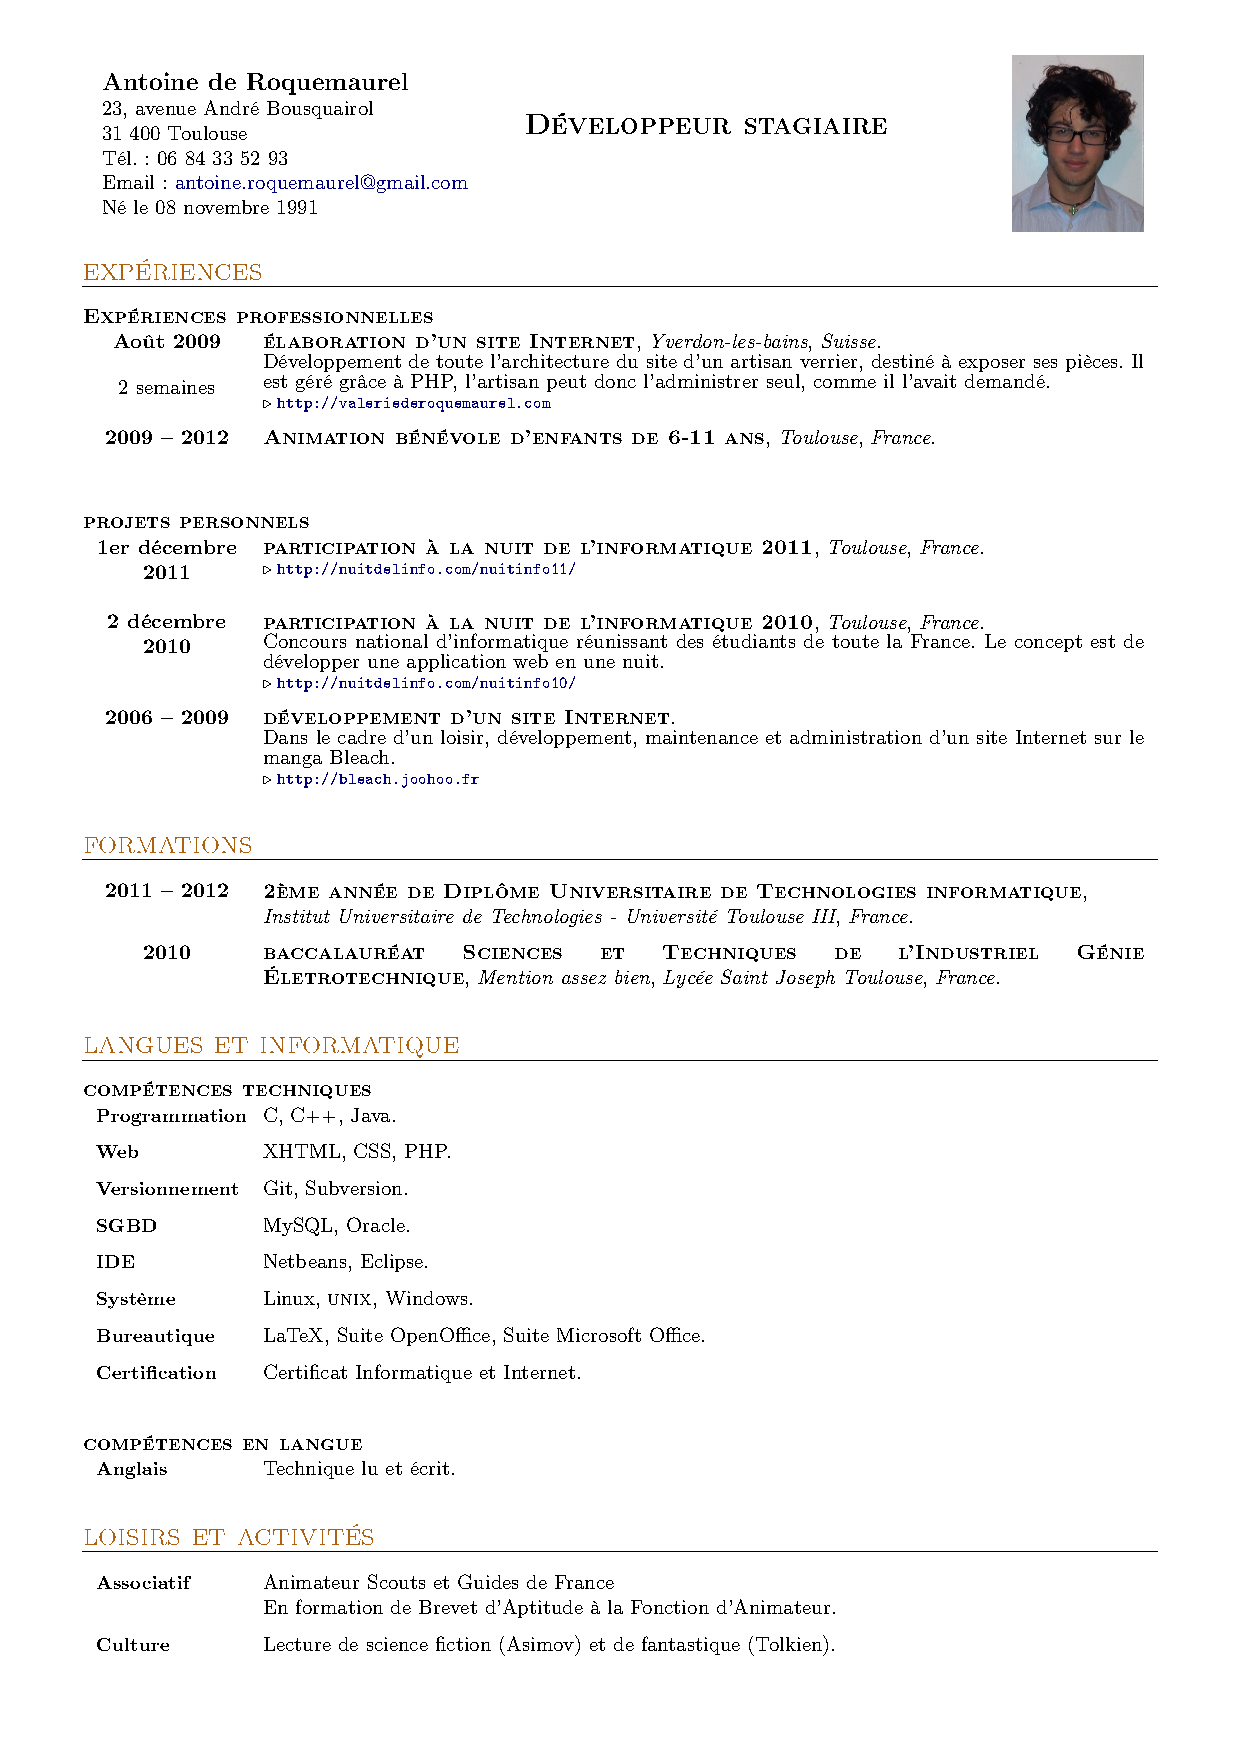
\includepdf{images/oldCV.pdf}
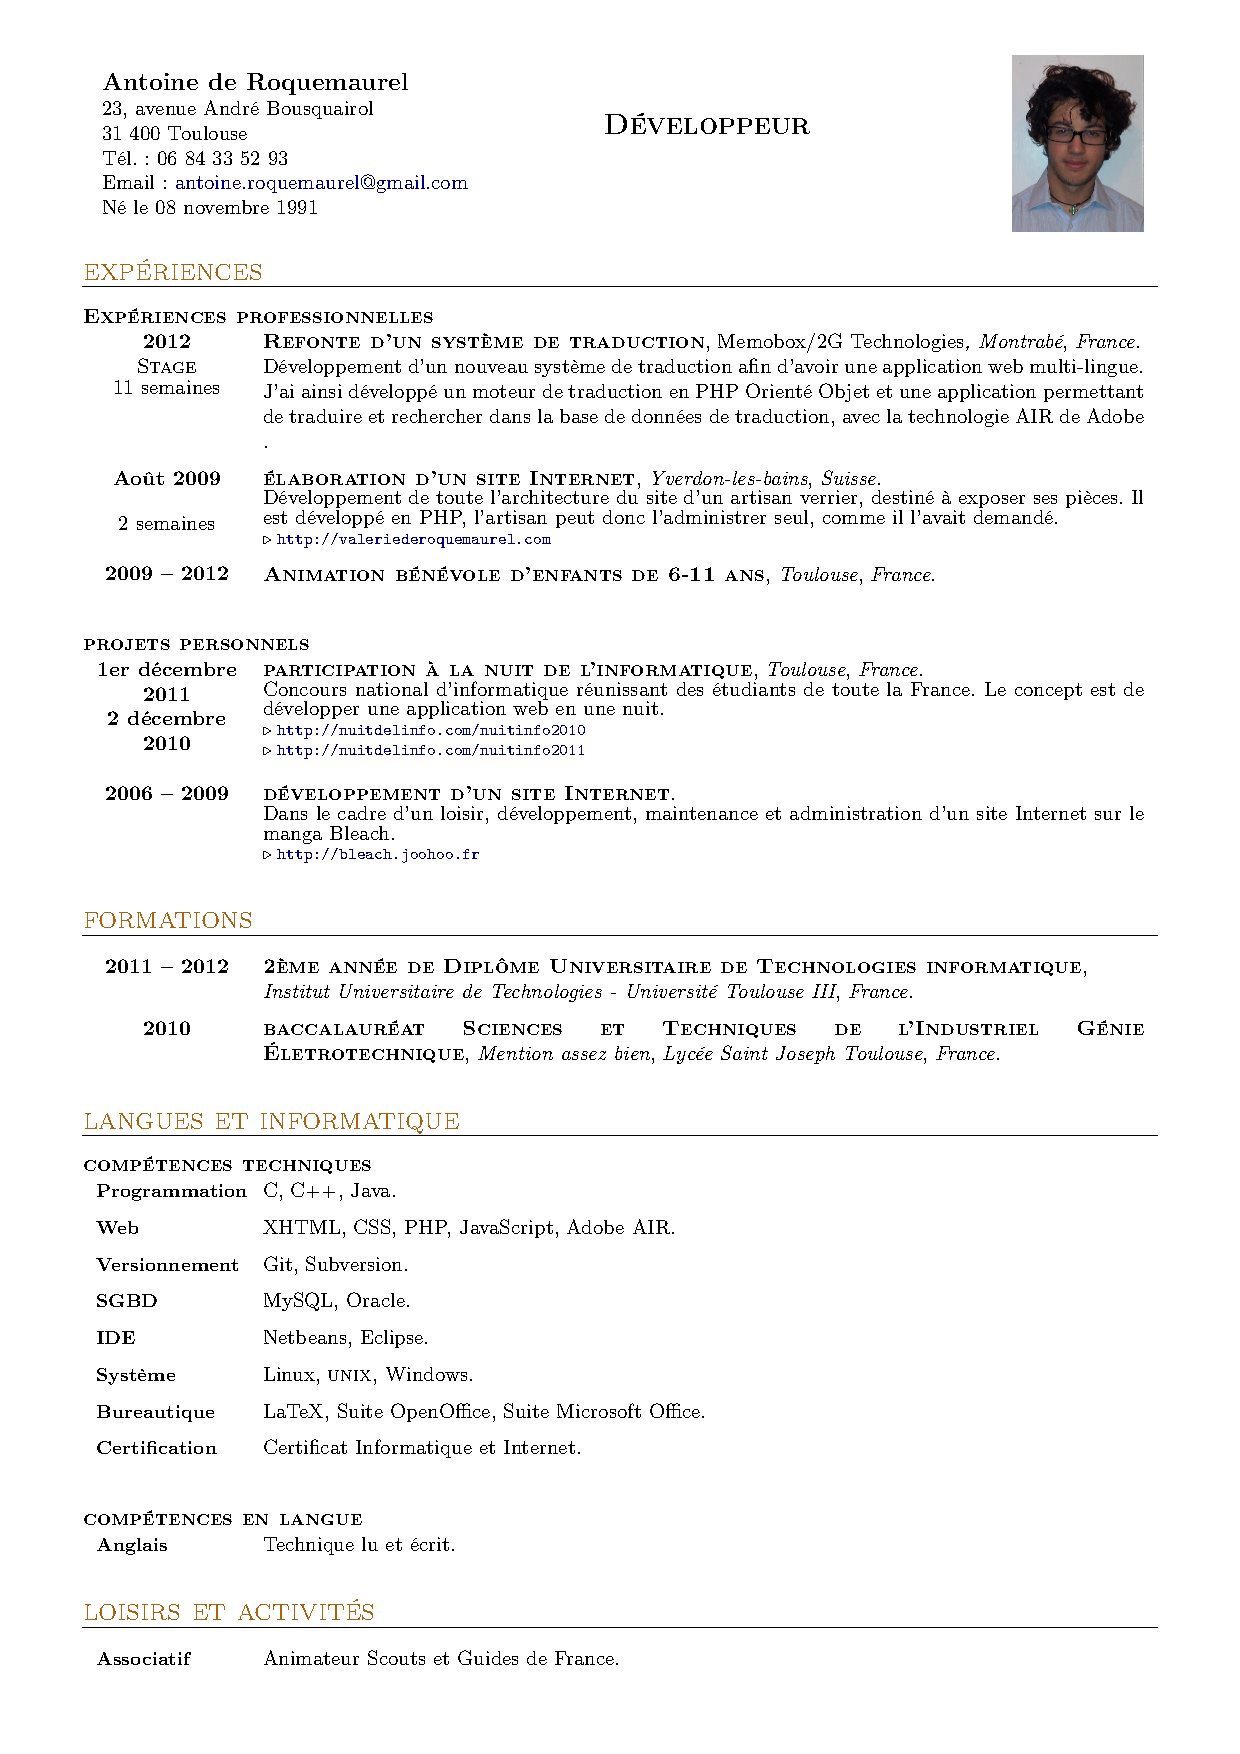
\includepdf{images/newCV.pdf}


		\cleardoublepage
	\setcounter{page}{1}
	\appendix
	\let\oldaddtocontents\addtocontents
	\def\addtocontents#1{%
		\def\tmpa{#1}%
		\def\tmpb{toc}%
		\ifx\tmpa\tmpb
		   \def\tmpa{toca}%
		\fi%
	 \expandafter\oldaddtocontents\expandafter{\tmpa}%
	 }


		
\includepdf{styles/couverture_annexes.pdf} %Couverture du rapport de stage
	\newpage
	\begin{flushright}
		~
		\vfill
		\vspace{200px}
		Version du \today{}
	\end{flushright}
	\thispagestyle{empty}
    \newpage
\sffamily
	\vspace{10px}
\thispagestyle{empty}
	%
	%
	% Pour éviter de créer un nouveau paragraph, on commente les lignes vide
		\vspace{30px}
		%
		\mbox{}\hfill{
			\begin{flushright}
				\fontsize{15}{15} \selectfont Antoine de \bsc{Roquemaurel}\\\vspace{10px}
				\fontsize{10}{10} \selectfont Stage effectué chez Memobox -- 2G technologies\\
				Du 10 Avril 2012 au 22 Juin 2012
			\end{flushright}
			\begin{flushleft}
				Pour M. Denis \bsc{Mallet}\\
				Pour M. Patrick \bsc{Magnaud}\\
			\end{flushleft}
		}\par
		%
		\vfill\mbox{}\vfill
		%
		%
		\vfill
		\vfill
		\vfill
		\vfill
		\vfill
		\hspace{65px}
		\fbox{
		\begin{minipage}{0.7\textwidth}
			\begin{center}
				\vspace{20px}	
				\fontsize{35}{25}\selectfont Rapport de stage
				
				\fontsize{22}{22}\selectfont \titreRapport
				\vspace{20px}	
			\end{center}
		\end{minipage}
		}
		%
%		\hrule height 4pt
		%
		\begin{center}
			\fontsize{20}{20}\selectfont\vspace{20px} --- Annexes ---
		\end{center}
		% Les vfill servent à insérer du blanc en dessous du titre pour éviter que le titre aille tout en bas
		% Plus il y a de vFill plus le titre sera haut dans la page
	% Le cadre sur la gauche, une boite rouge avec les logos IUT et UPS
		\vfill
		\vfill
		\vfill
		\vfill
		\vfill
		\vfill
		\vfill
	\begin{flushleft}
		\fontsize{11.5}{11.5}\selectfont
		Memobox -- 2G Technologies\\
		12 Bv de l'Europe\\
		31850 -- \bsc{Montrabé}\\
		
\includegraphics[width=4.5cm]{images/logoMemobox.png}\\%
	\end{flushleft}
		\vfill
		\vfill
		\vfill
		\vfill
		\mbox{}
		
\newpage
~
\thispagestyle{empty}

	 \tableofcontentsA
	 \newpage
	\thispagestyle{empty}
	\renewcommand{\chaptermark}[1]{\markboth{\bsc{Annexe~\thechapter{} :} #1}{}}
	\chapter{Résultats}
    \section{MemoLanguage}
    \subsection{Recherche}
    \begin{figure}[H]
        \centering
        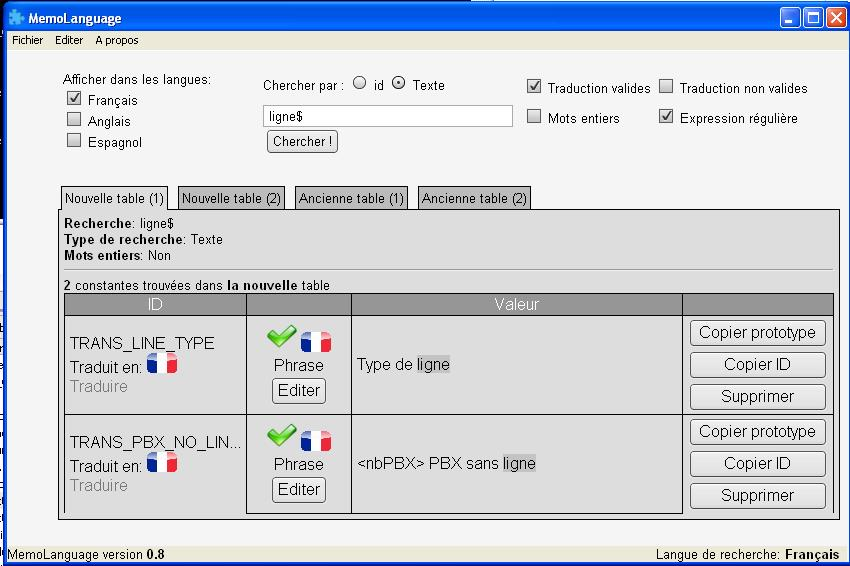
\includegraphics[width=16cm]{images/2-activite/searchRegex.jpg}\label{searchRegex}
        sur cette capture, on peut voir les différentes case à cocher permettant d'affiner la recherche.

            \'Egalement, 4 onglets sont présents, suivant sur l'onglet où on se trouve, cela cherchera dans la nouvelle table ou dans l'ancienne table, comme indiqué par l'onglet.

            La présence de plusieurs onglets, permet de ne pas effacer une recherche qui est intéressante.

        \caption{Recherche avec expression régulière}
    \end{figure}

    \subsection{\'Edition}
        \begin{figure}[H]
            \centering
            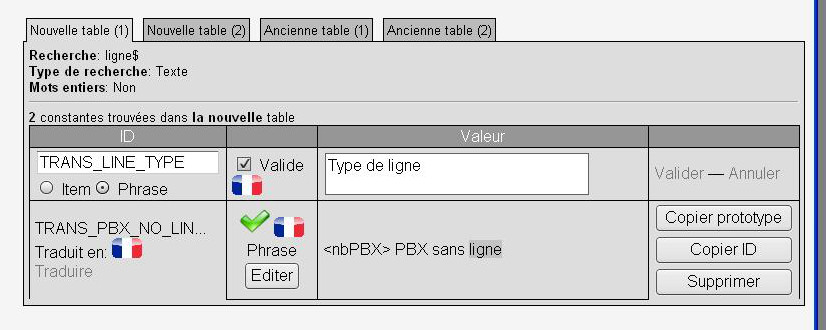
\includegraphics[width=16cm]{images/2-activite/edition.jpg}
            \caption{\'Edition d'une constante}
            \label{edition}
        \end{figure}
    \subsection{Ajout de constante}
    \label{ajoutCst}
        \begin{figure}[H]
            \centering
            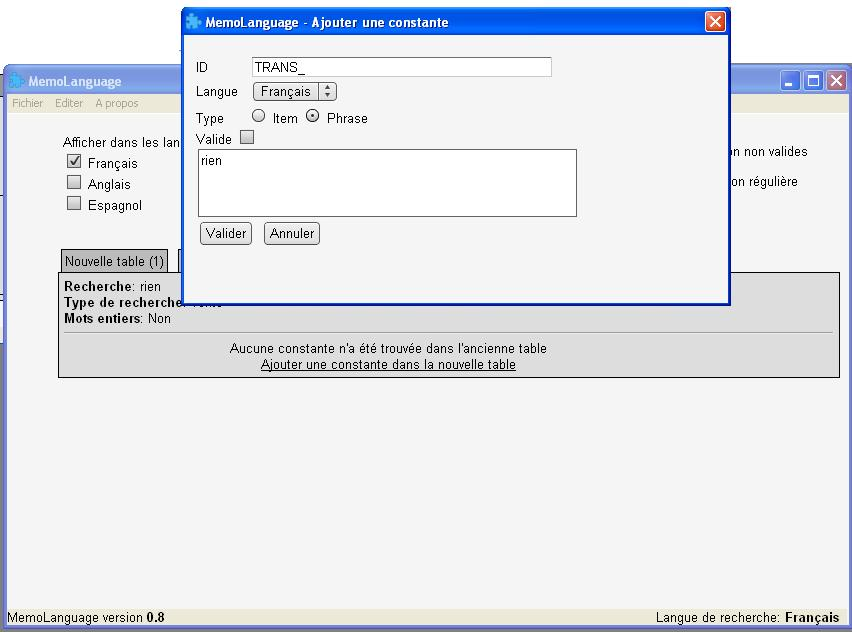
\includegraphics[width=16cm]{images/2-activite/ajoutCst.jpg}

            Sur cette capture d'écran, l'utilisateur à effectuer la recherche ''rien`` et n'a trouvé aucune correspondance, ainsi il a cliquer sur le lient ''Ajouter une constante dans la nouvelle table`` ce qui lui a ouvert la fenêtre avec le champ de valeur pré-remplit avec ''rien``.
            Le nom d'ID est également pré-remplit avec \texttt{TRANS\_} afin d'inciter les développeurs à utiliser ce préfixe.
            \caption{Ajouter d'une constante après une recherche infructueuse}
        \end{figure}
    \subsection{Suppression}
    \label{suppression}
        \begin{figure}[H]
        \centering
        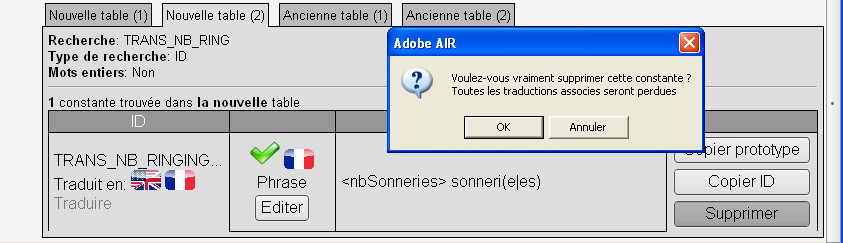
\includegraphics[width=16cm]{images/2-activite/suppression.jpg}
        \caption{Suppression d'une constante}
    \end{figure}
        \subsection{Copier vers nouvelle table}
    \begin{figure}[H]
        \centering
        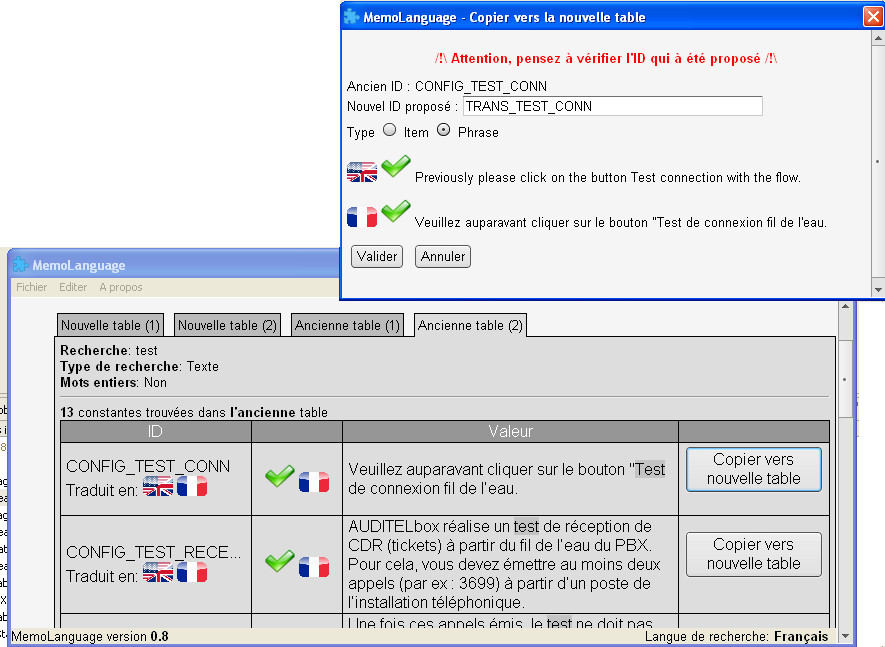
\includegraphics[width=16cm]{images/2-activite/copierVersNouvelleTable.jpg} \caption{Basculer une constante de l'ancienne base vers la nouvelle}
        \label{copierVersNouvelleTable}
        Dans cette capture d'écran, on remarque qu'automatiquement un nouvel ID est proposé afin de garder la cohérence avec les préfixe, cependant une invitation à vérifier et indiquer au développeur.
    \end{figure}

    \subsection{Traduction}
    \label{traduction}
    \begin{figure}[H]
        \centering
        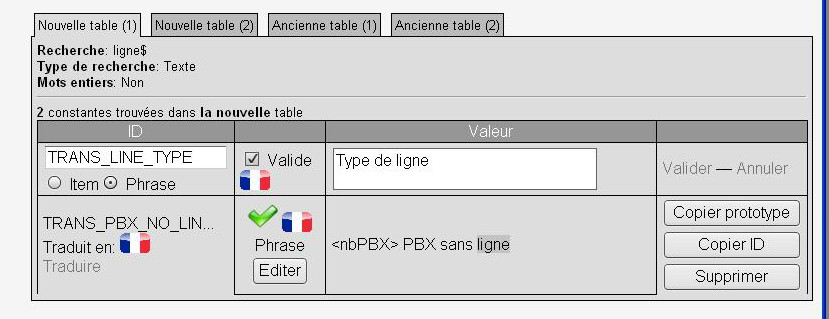
\includegraphics[width=16cm]{images/2-activite/traduction.jpg}
        \caption{Traduction d'une constante}
    \end{figure}

    \subsection{Champs TranslatedText\_short et TranslatedText\_long}
    \label{nouveauxScreens}
        \begin{figure}[H]
        \centering
        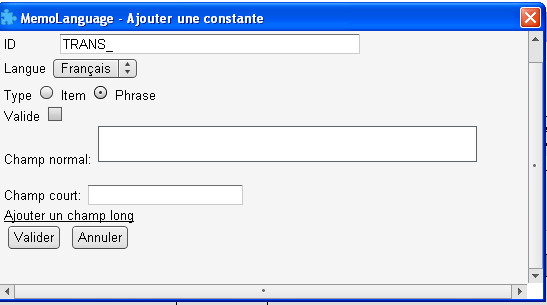
\includegraphics[width=16cm]{images/annexes/resultats/nouvelleInsertion.jpg} 
        \caption{Insertion d'une constante}
        \label{champCourtLong}
    \end{figure}
    \begin{figure}[H]
        \centering
        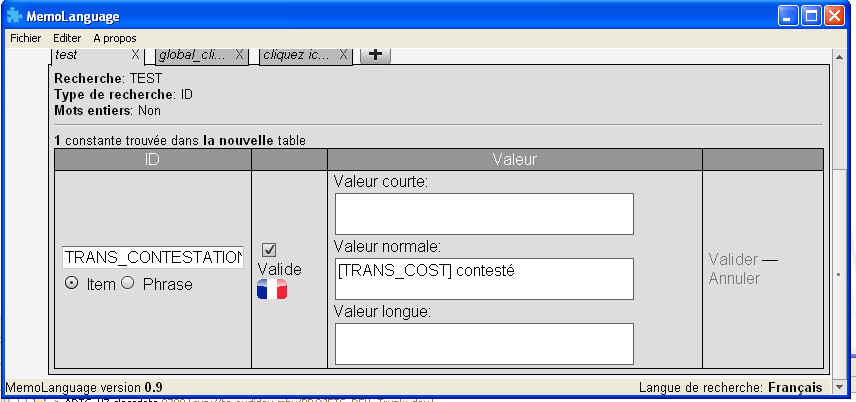
\includegraphics[width=16cm]{images/annexes/resultats/nouvelleEdition.jpg}
        \caption{\'Edition d'une constante}
    \end{figure}
        \section{\adt{} multilingue}
        \begin{figure}[H]
        \centering
        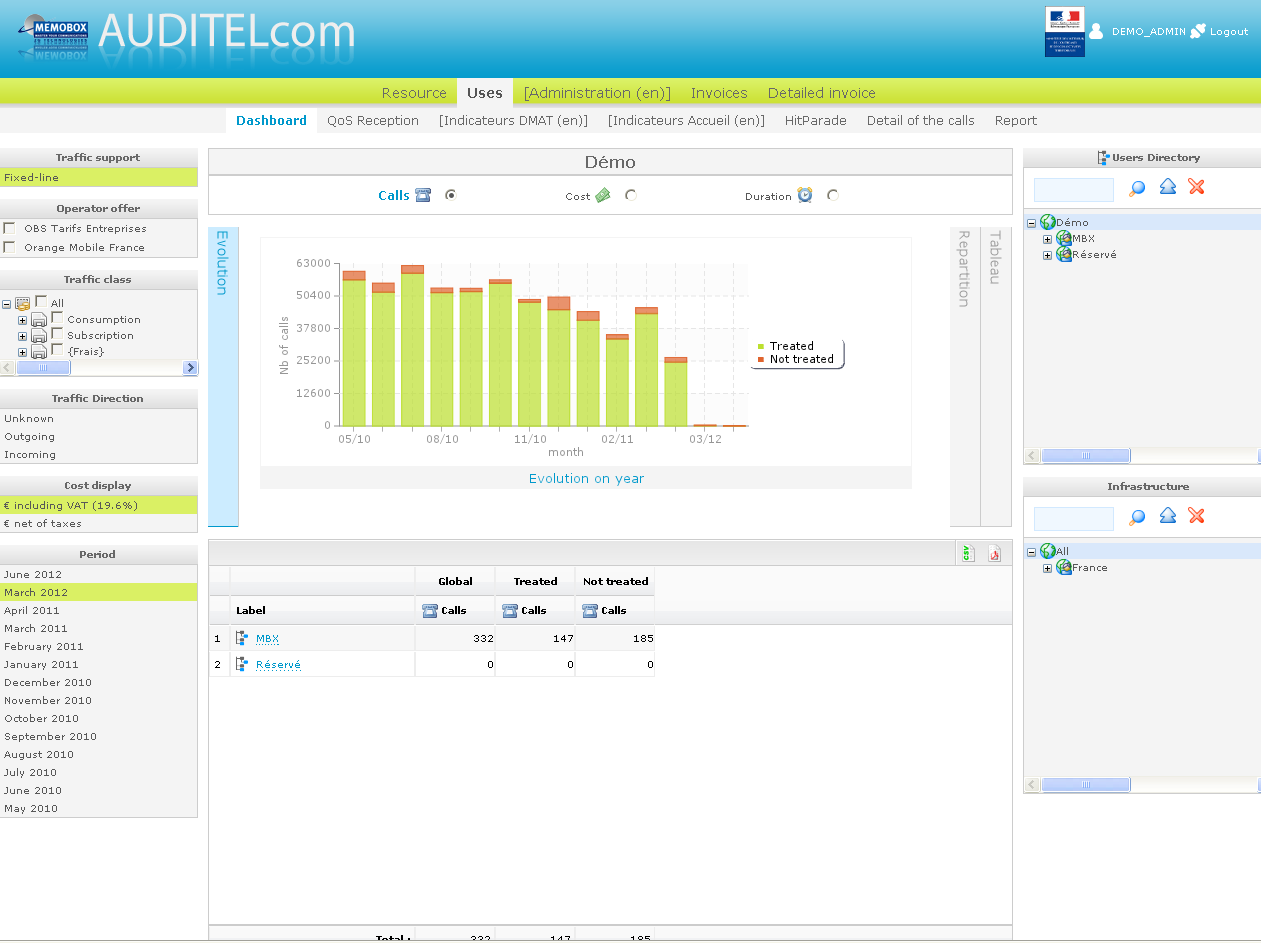
\includegraphics[angle=90,width=16.5cm]{images/annexes/resultats/adtAnglais.png}
        \caption{\adt{} en anglais}
        \label{adtAnglais}
    \end{figure}
            Comme vous pouvez le voir, l'intégration n'est pas finit, certains mots s'affichent en français, cependant une grande partie du travail à été fait.




    

        \listoffigures
     \listoftables
    \lstlistoflistings
	\chapter{Code source}
\section{Moteur de traduction}
    \lstinputlisting[language=PHP, caption=TLanguage.class.php]{contenu/annexes/TLanguage.class.php} %
\section{Memolanguage}
    \subsection{Le serveur} %% TODO, cacher mdp
%    \lstinputlisting[language=PHP, caption=databaseChanges.class.php]{contenu/annexes/MemoLanguage_Serveur/databaseChanges.class.php}
\lstinputlisting[language=PHP, caption=database.class.php]{contenu/annexes/MemoLanguage_Serveur/database.class.php}%
%\lstinputlisting[language=PHP, caption=databaseSchemaTable.class.php]{contenu/annexes/MemoLanguage_Serveur/databaseSchemaTable.class.php}
\lstinputlisting[language=PHP, caption=databaseSearch.class.php]{contenu/annexes/MemoLanguage_Serveur/databaseSearch.class.php}
\lstinputlisting[language=PHP, caption=index.php]{contenu/annexes/MemoLanguage_Serveur/index.php}%
\lstinputlisting[language=PHP, caption=page.class.php]{contenu/annexes/MemoLanguage_Serveur/page.class.php}%
%\lstinputlisting[language=PHP, caption=pagedelete.class.php]{contenu/annexes/MemoLanguage_Serveur/pagedelete.class.php}
%\lstinputlisting[language=PHP, caption=pageinsert.class.php]{contenu/annexes/MemoLanguage_Serveur/pageinsert.class.php}
\lstinputlisting[language=PHP, caption=pageselect.class.php]{contenu/annexes/MemoLanguage_Serveur/pageselect.class.php}%
%\lstinputlisting[language=PHP, %caption=pageupdate.class.php]{contenu/annexes/MemoLanguage_Serveur/pageupdate.class.php}
%\lstinputlisting[language=PHP, caption=util.class.php]{contenu/annexes/MemoLanguage_Serveur/util.class.php}

\subsection{Le client}
    \subsubsection{lib}
%\lstinputlisting[language=JavaScript, caption=AIRAliases.js]{contenu/annexes/MemoLanguage_Client/AIRAliases.js}
%
%\lstinputlisting[language=JavaScript, caption=addCells.js]{contenu/annexes/MemoLanguage_Client/addCells.js}
 %  \lstinputlisting[language=JavaScript,  caption=configuration.js]{contenu/annexes/MemoLanguage_Client/configuration.js}
%\lstinputlisting[language=JavaScript, caption=copyToNewTable.js]{contenu/annexes/MemoLanguage_Client/copyToNewTable.js}
%\lstinputlisting[language=JavaScript, caption=menu.js]{contenu/annexes/MemoLanguage_Client/menu.js}
%\lstinputlisting[language=, caption=packaging.bat]{contenu/annexes/MemoLanguage_Client/packaging.bat}
\lstinputlisting[language=JavaScript, caption=search.js]{contenu/annexes/MemoLanguage_Client/search.js}%
%\lstinputlisting[language=JavaScript, caption=systray.js]{contenu/annexes/MemoLanguage_Client/systray.js}
%\lstinputlisting[language=JavaScript, caption=tabs.js]{contenu/annexes/MemoLanguage_Client/tabs.js}
%\lstinputlisting[language=JavaScript, caption=traduction.js]{contenu/annexes/MemoLanguage_Client/traduction.js}
%\lstinputlisting[language=JavaScript, caption=util.js]{contenu/annexes/MemoLanguage_Client/util.js}
%\lstinputlisting[language=JavaScript, caption=variablesGlobales.js]{contenu/annexes/MemoLanguage_Client/variablesGlobales.js}
%\lstinputlisting[language=JavaScript, caption=actionAddCst.js]{contenu/annexes/MemoLanguage_Client/actionAddCst.js}
%\lstinputlisting[language=JavaScript, caption=actionCopy.js]{contenu/annexes/MemoLanguage_Client/actionCopy.js}
%\lstinputlisting[language=JavaScript, caption=actionSearch.js]{contenu/annexes/MemoLanguage_Client/actionSearch.js}
%\lstinputlisting[language=JavaScript, caption=actionTabs.js]{contenu/annexes/MemoLanguage_Client/actionTabs.js}
\lstinputlisting[language=JavaScript, caption=actionTranslate.js]{contenu/annexes/MemoLanguage_Client/actionTranslate.js}
%\lstinputlisting[language=JavaScript, caption=actionUpdates.js]{contenu/annexes/MemoLanguage_Client/actionUpdates.js}

 %   \subsubsection{html}
%\lstinputlisting[language=HTML, caption=about.html]{contenu/annexes/MemoLanguage_Client/about.html}
%    \lstinputlisting[language=HTML, caption=addCst.html]{contenu/annexes/MemoLanguage_Client/addCst.html}
%\lstinputlisting[language=HTML, caption=changeConfig.html]{contenu/annexes/MemoLanguage_Client/changeConfig.html}
%\lstinputlisting[language=HTML, caption=copyToNewTable.html]{contenu/annexes/MemoLanguage_Client/copyToNewTable.html}
\lstinputlisting[language=HTML, caption=Page HTML principale homeSearch.html]{contenu/annexes/MemoLanguage_Client/homeSearch.html}

    \subsubsection{bin}
\lstinputlisting[language=XML, caption=Descripteur de fichier MemoLanguage-app.xml]{contenu/annexes/MemoLanguage_Client/MemoLanguage-app.xml}%



\end{document}






